\documentclass[10pt,t]{beamer}

\usetheme{lmtslides}
\usepackage{eso-pic}
\usepackage{graphicx}
\usepackage{times}
\usepackage[latin1]{inputenc}
\usepackage[amssymb]{SIunits}
\usepackage{amsmath,amssymb}
\usepackage{eurosym}
\usepackage{booktabs}
\usepackage{colortbl}
\usepackage{url}
\usepackage[absolute,overlay]{textpos}
\usepackage{graphicx}
\usepackage{mathtools}
\usepackage{pifont}
\usepackage{appendixnumberbeamer}
\usepackage{subcaption}
\usepackage{amssymb,amsmath,mleftright,mathtools}
\usepackage{cite}
\usepackage[T1]{fontenc}
\usepackage{hyperref}
\usepackage{amsmath,amssymb,amsfonts}
\usepackage{array,booktabs}
\usepackage{algorithm}
\usepackage{algpseudocode} 
\usepackage{algorithmicx}
\usepackage{listings}
\usepackage{textcomp}
\usepackage{url}
\usepackage{caption} 
\usepackage{tcolorbox}
\usepackage{empheq}
\usepackage{varwidth}
\usepackage{balance}
\usepackage{flushend} 
\usepackage{stfloats}
\usepackage{multimedia} % For embedding videos
\usepackage{emoji}

% TikZ for diagrams
\usepackage{tikz}
\usetikzlibrary{arrows.meta,shapes,positioning}
\usetikzlibrary{calc,angles,quotes}

% --- Macro for drawing a 2D spherocylinder ---
% #1 = center coordinate
% #2 = rotation angle
% #3 = half-length
% #4 = radius

\newcolumntype{M}[1]{>{\centering\arraybackslash}m{#1}}

\newcommand{\drawSpherocyl}[4]{
    \begin{scope}[shift={(#1)},rotate=#2]
        \draw[line width=1pt,rounded corners=6pt] (-#3 + #4,#4) -- (#3 - #4,#4);
        \draw[line width=1pt,rounded corners=6pt] (-#3 + #4,-#4) -- (#3 - #4,-#4);
        \draw[line width=1pt,rounded corners=6pt] (#3 - #4,-#4) arc[start angle=-90,end angle=90,radius=#4];
        \draw[line width=1pt,rounded corners=6pt] (-#3 + #4,#4) arc[start angle=90,end angle=270,radius=#4];
        \fill [black] (#1) circle (2pt);
    \end{scope}
}



\DeclareMathAlphabet\mathbfcal{OMS}{cmsy}{b}{n}

\setbeamertemplate{caption}{\raggedright\insertcaption\par}
\setbeamertemplate{bibliography item}[online]
\graphicspath{{figures/}}

\setlang{en}	

\newcommand{\xmark}{\ding{55}}%
\newcommand{\cmark}{\ding{51}}%

\renewcommand{\footnoterule}{\vfill\kern -3pt  \kern 2.6pt}

\setbeamertemplate{caption}{\raggedright\insertcaption\par}
\setbeamertemplate{bibliography item}[online]
\graphicspath{{figures/figures_paper/}}

\title{Proliferating Cell Collectives:\newline A Comparison of Hard and Soft Collision Models}
\type{Sf}
\author{Manuel Lerchner}
\email{manuel.lerchner@tum.de}
\advisorOne{Samuel James Newcome}
\advisorTwo{}
\date{\today}

\AtBeginSection[]
{
    \begin{frame}
        \frametitle{Outline}
        \tableofcontents[currentsection,currentsubsection]
    \end{frame}
}

\begin{document}

\maketitle

\setcounter{framenumber}{0}

% ============================================================
% SECTION 1: MOTIVATION & CONTEXT
% ============================================================

\section{Motivation}

\begin{frame}
    \frametitle{Computational Biology: A Growing Field}

    \begin{columns}
        \begin{column}{0.58\textwidth}
            \textbf{Why simulate biological systems?}
            \begin{itemize}
                \item Link micro-to macroscopic behavior
                \item Test hypotheses in silico
                \item Guide experimental design
                \item Often just look beautiful
            \end{itemize}

            \vspace{0.3cm}

            \textbf{The computational challenge:}
            \begin{itemize}
                \item Large system sizes
                \item Complex interactions
                \item Long timescales
            \end{itemize}
        \end{column}

        \begin{column}{0.5\textwidth}
            \centering
            \begin{figure}
                \centering
                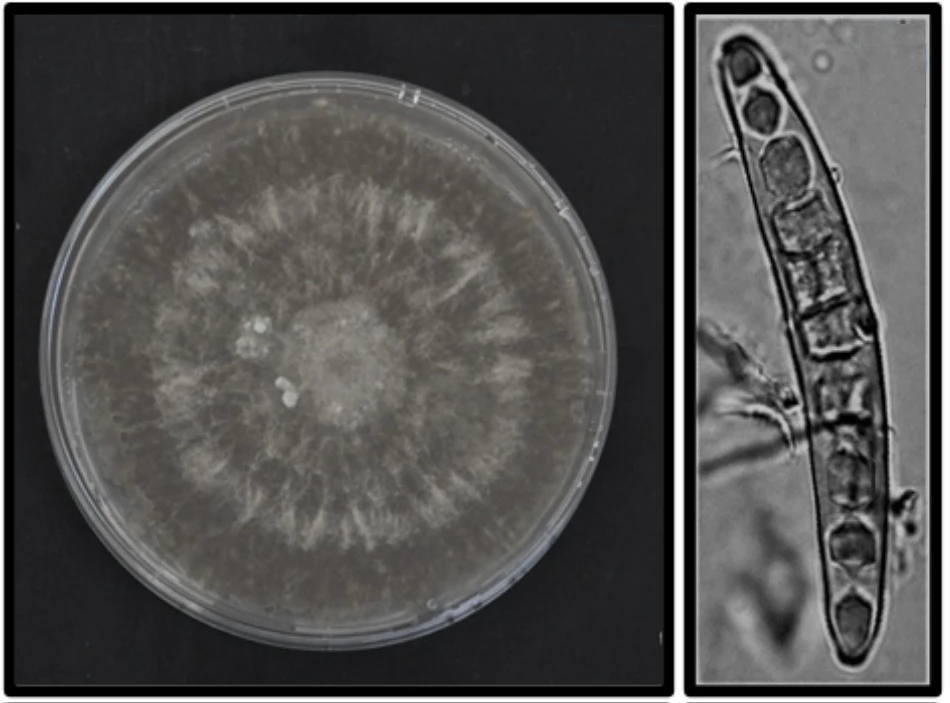
\includegraphics[width=\textwidth]{figures/figures_paper/real-bacteria/Exserohilum turcicum.png}
                \caption*{\scriptsize{Real fungal colony showing ring patterns~\cite{Bankole2023}.}}
            \end{figure}
        \end{column}
    \end{columns}

\end{frame}

\begin{frame}
    \frametitle{The Performance Gap in Biological Modeling}

    \begin{block}{Common Practice: Focus on Biological Insight}
        \begin{itemize}
            \item Pick a model that \textit{can} reproduce qualitative behavior.
            \item Tune parameters until the output ``looks right''.
            \item Publish biological findings.
            \item \textbf{Runtime? Scaling?, Source Code?} Often unreported.
        \end{itemize}
    \end{block}

    \vspace{0.1cm}

    \begin{alertblock}{The Neglected Computational Core}
        \begin{itemize}
            \item \textbf{Algorithmic Efficiency:} Can we optimize further?
            \item \textbf{Performance Scaling:} How does it handle larger systems?
            \item \textbf{Speed vs. Accuracy:} What are the concrete trade-offs?
            \item \textbf{Model Comparisons:} Are different methods equivalent?
        \end{itemize}
    \end{alertblock}
\end{frame}

\begin{frame}
    \frametitle{This Work: Comparing Collision Models}

    \begin{columns}
        \begin{column}{0.6\textwidth}
            \textbf{Research Questions:}
            \begin{enumerate}
                \item Do different collision models produce the same biological patterns?
                      \begin{itemize}
                          \item Ring formation
                          \item Microdomain structure
                          \item Cell density
                      \end{itemize}
                \item Which model is faster?
                \item Which approach scales better?
                \item When should each be used?
            \end{enumerate}
        \end{column}

        \begin{column}{0.4\textwidth}

            \vspace{-0.8cm}
            \begin{figure}
                \centering
                \begin{subfigure}{0.63\textwidth}
                    \centering
                    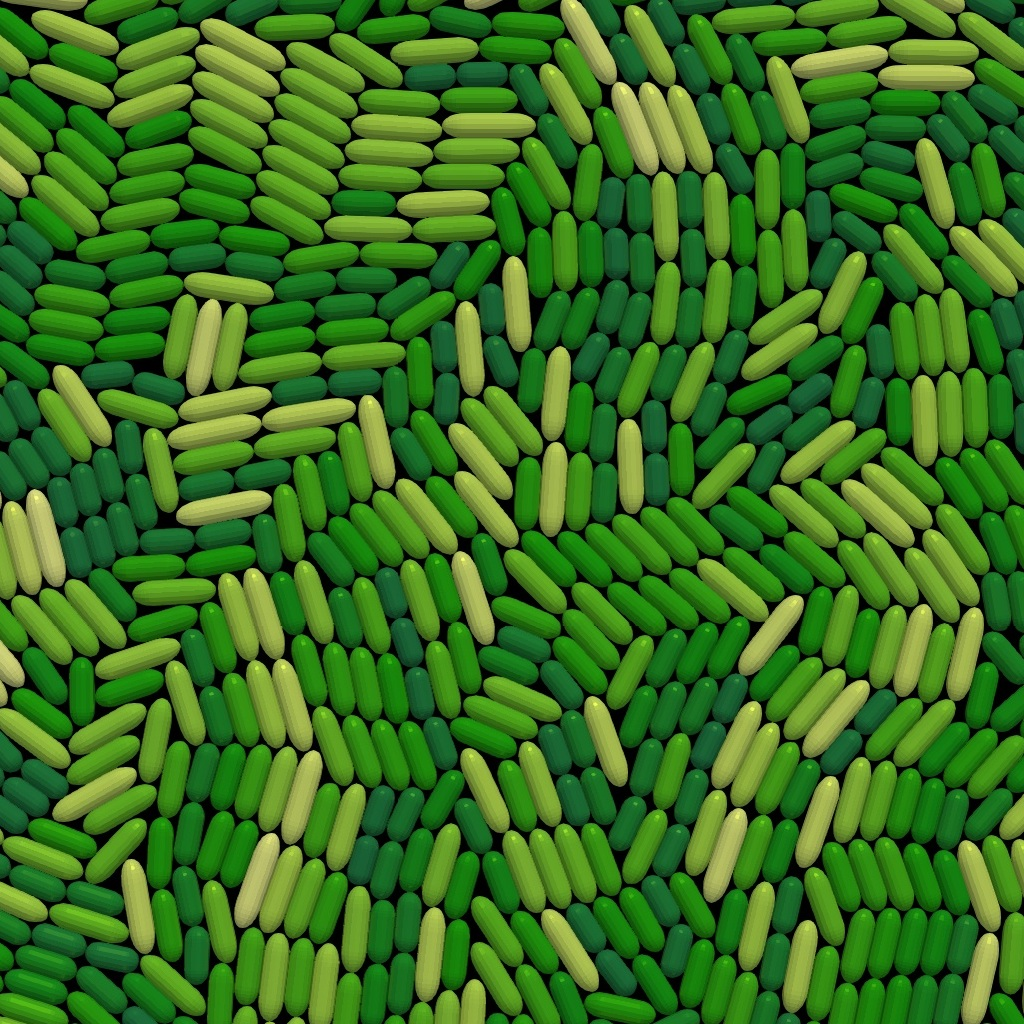
\includegraphics[width=\textwidth]{figures/figures_paper/comparison_plots/density_hard.jpeg}
                    \caption{{Model 1}}
                \end{subfigure}
                \vfill
                \begin{subfigure}{0.63\textwidth}
                    \centering
                    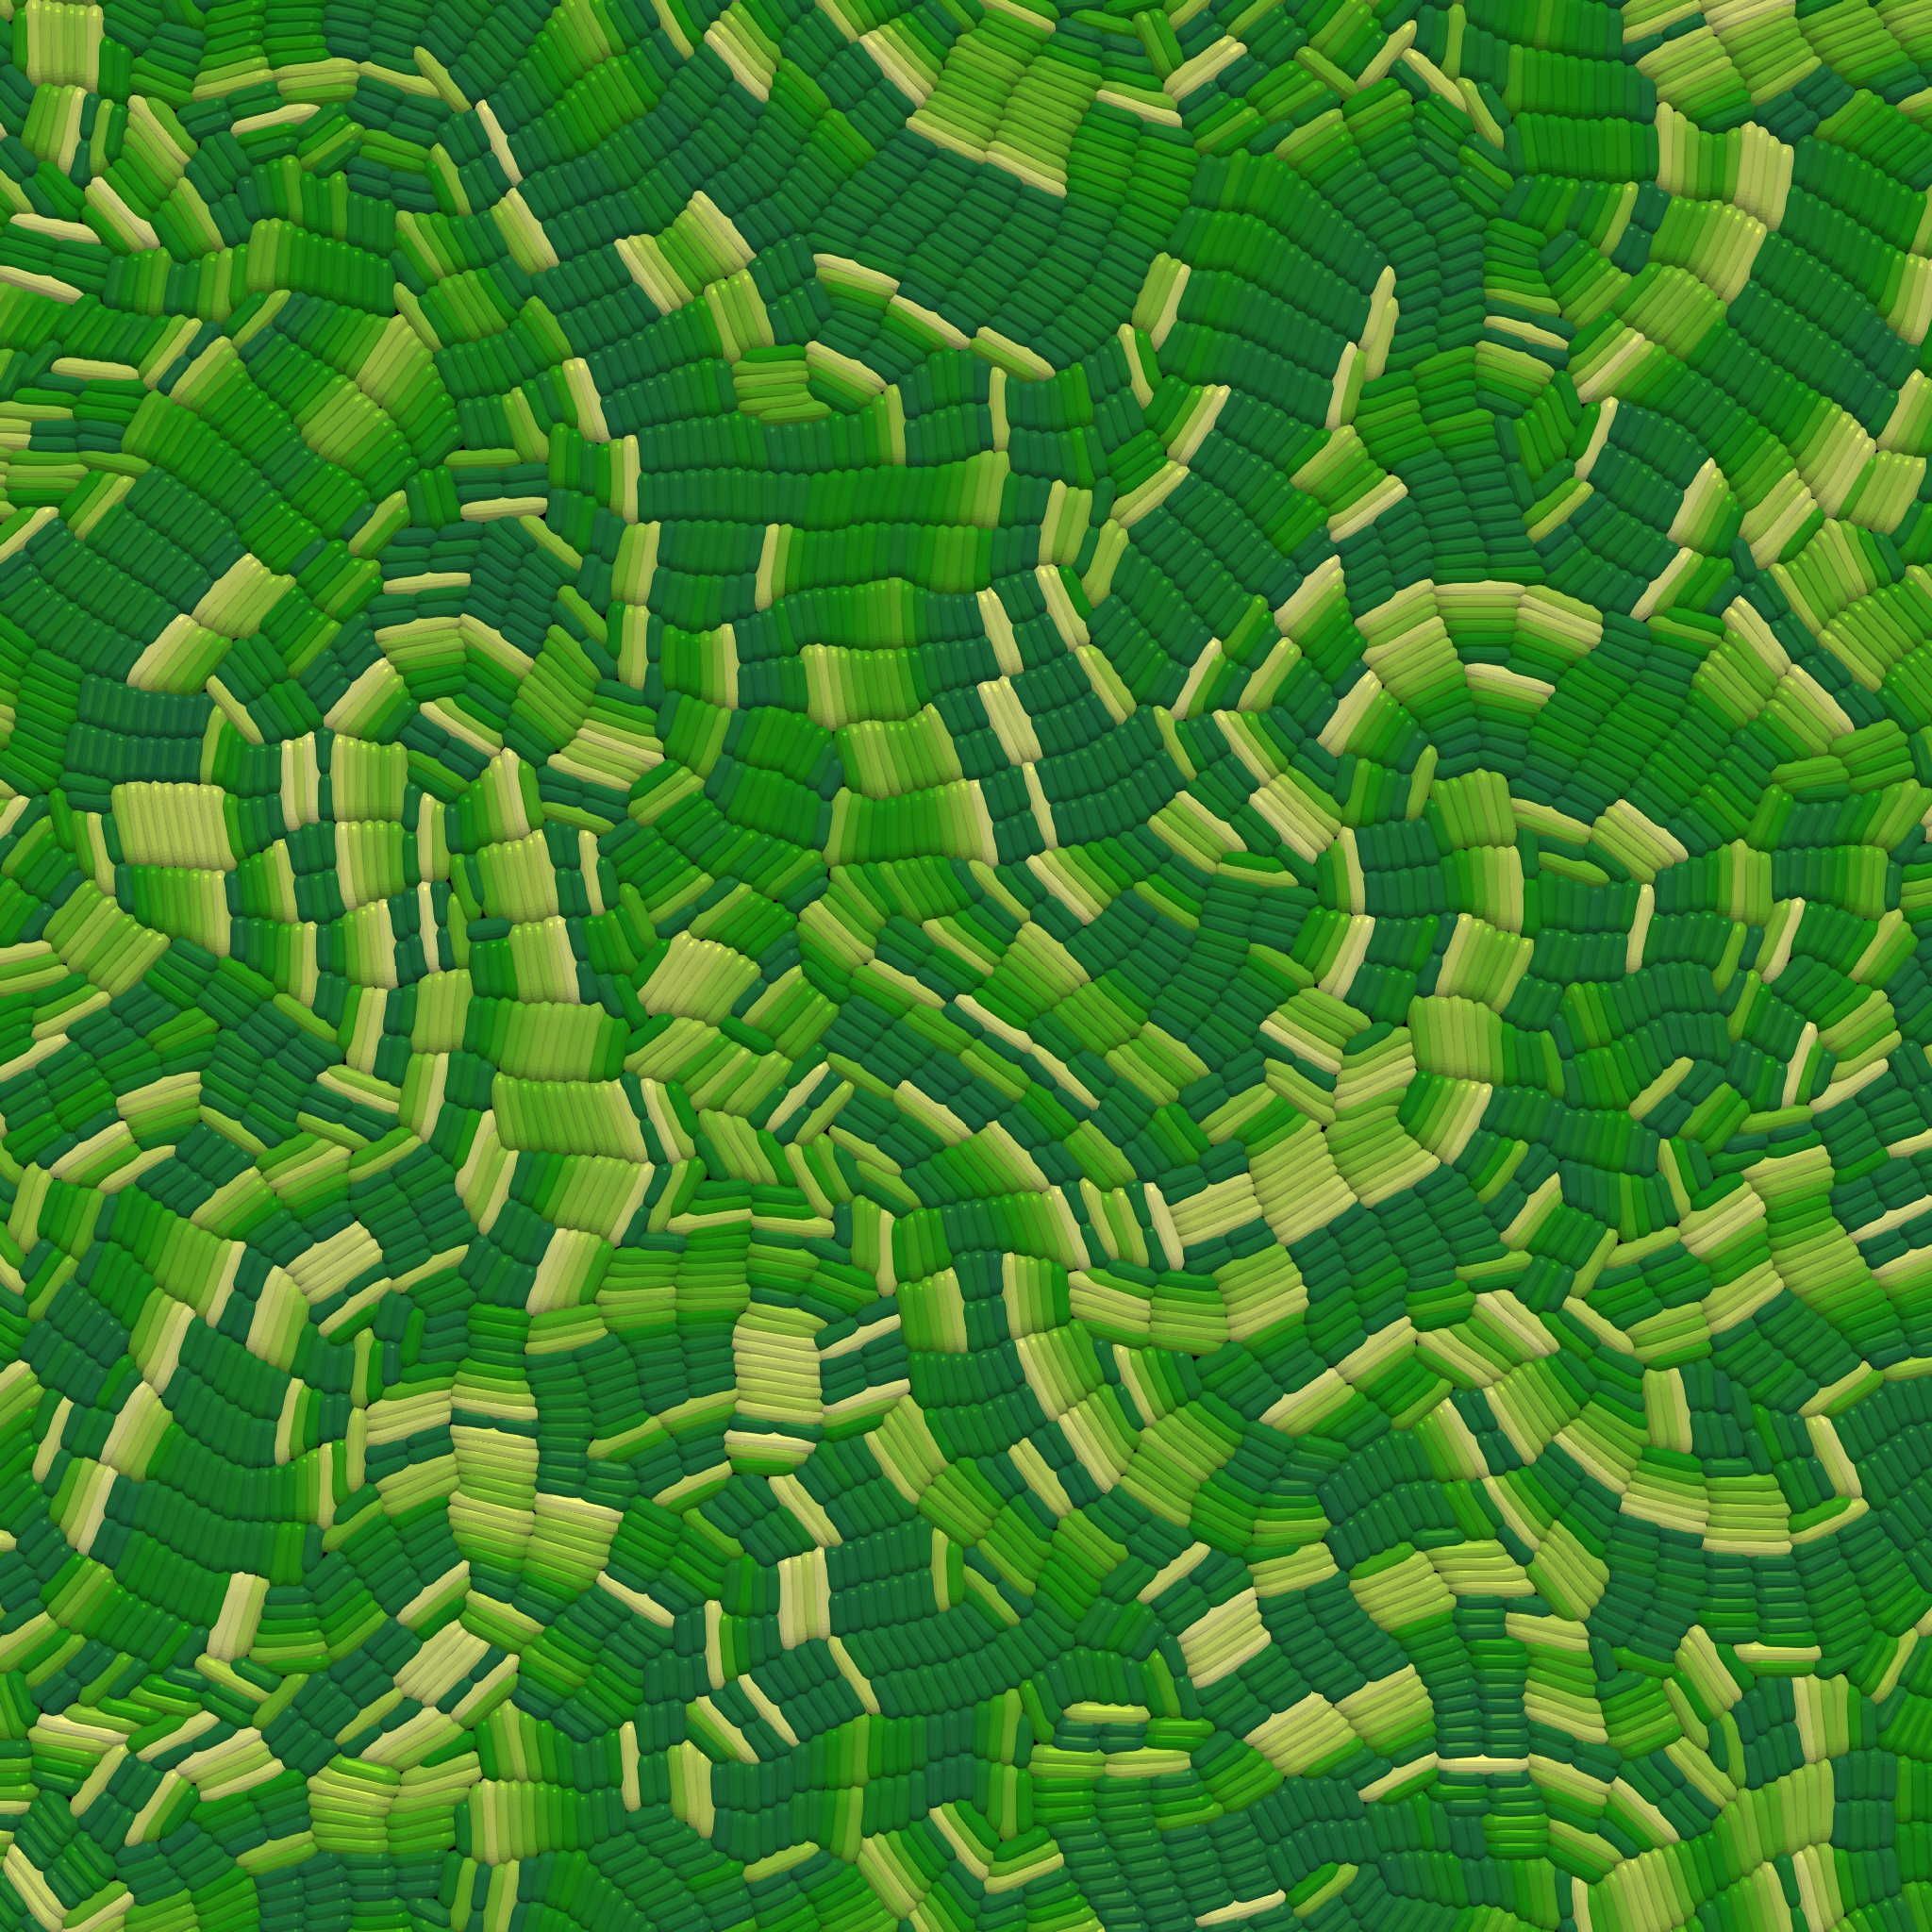
\includegraphics[width=\textwidth]{figures/figures_paper/comparison_plots/density_soft.jpeg}
                    \caption{{Model 2}}
                \end{subfigure}
            \end{figure}
        \end{column}
    \end{columns}

\end{frame}

% ============================================================
% SECTION 2: BIOLOGICAL SYSTEM
% ============================================================

\section{The Biological System}

\begin{frame}
    \frametitle{Core Biological Mechanism}

    \begin{center}
        \begin{tikzpicture}[node distance=3cm, auto]
            \tikzstyle{block} = [rectangle, draw, fill=blue!20, text width=6em, text centered, rounded corners, minimum height=3em]
            \tikzstyle{arrow} = [thick,->,>=stealth]
            \tikzstyle{redarrow} = [line width=2pt, red, ->,>=stealth]

            \node [block] (growth) {Cell Growth and Division};
            \node [block, right of=growth] (collision) {Collisions};
            \node [block, below of=collision] (stress) {Mechanical Stress};
            \node [block, left of=stress] (inhibit) {Growth Inhibition};

            \draw [arrow] (growth) -- (collision);
            \draw [redarrow] (collision) -- (stress);
            \draw [arrow] (stress) -- (inhibit);
            \draw [arrow] (inhibit) -- (growth);
        \end{tikzpicture}
    \end{center}

    \vspace{0.2cm}

    \begin{itemize}
        \item We compare two methods to turn collisions into forces.
    \end{itemize}

\end{frame}

% ============================================================
% SECTION 3: MATHEMATICAL MODEL
% ============================================================

\section{Mathematical Framework}

\begin{frame}
    \frametitle{Cell Representation}

    \begin{itemize}
        \item Length $\ell(t)$ grows over time
        \item Diameter $d = 0.5$ fixed
        \item Position $\mathbf{x} \in \mathbb{R}^3$, Orientation $\mathbf{q} \in \mathbb{R}^4$
        \item Divide at $\ell_\text{crit} = 2 \ell_0$
        \item Contacts produce forces $\mathbf{F}_{ij}$ and torques
    \end{itemize}

    \vspace{.7cm}

    \begin{center}
        \begin{figure}
            \centering
            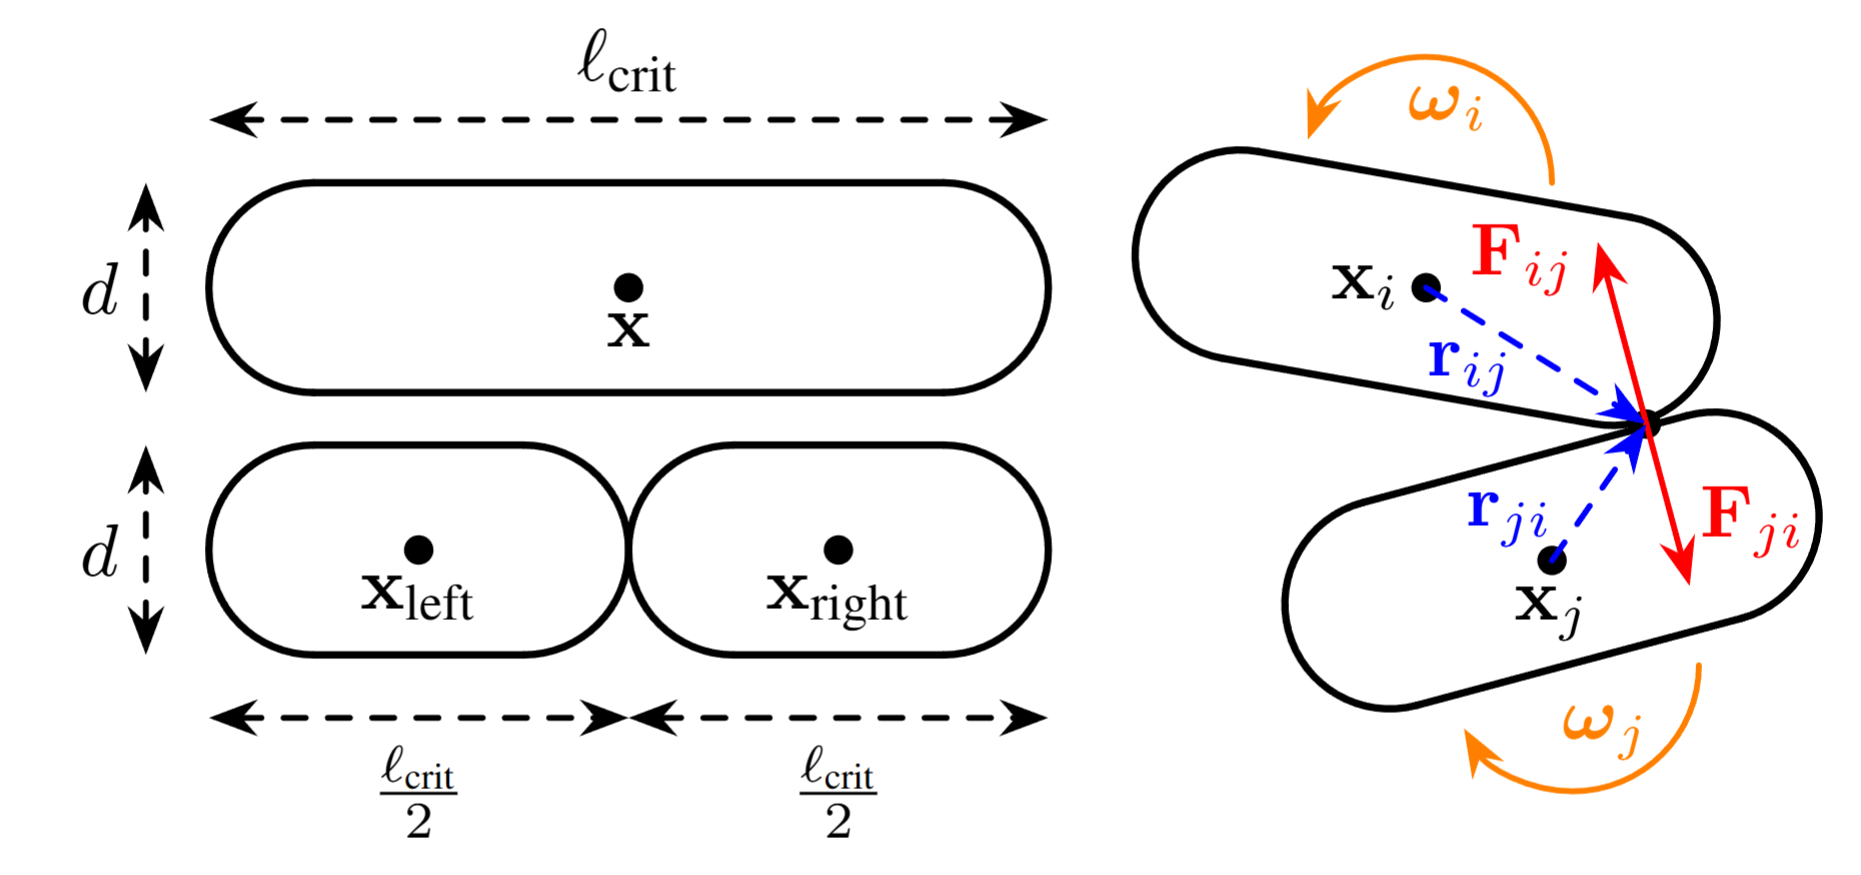
\includegraphics[width=0.6\textwidth]{figures/spherocylinder_model.png}
        \end{figure}
    \end{center}

\end{frame}

\begin{frame}
    \frametitle{Equations of Motion}

    \textbf{Overdamped dynamics (Re $\ll$ 1):}
    \begin{itemize}
        \item Viscous forces dominate, inertia negligible
        \item Cells behave like ``swimmers in honey''
    \end{itemize}

    \textbf{Translational motion:}
    \begin{equation*}
        \mathbf{u}_i = \frac{1}{\zeta \ell_i} \sum_{j \neq i} \mathbf{F}_{ij}
    \end{equation*}

    \textbf{Rotational motion:}
    \begin{equation*}
        \boldsymbol{\omega}_i = \frac{12}{\zeta \ell_i^3} \sum_{j \neq i} \mathbf{r}_{ij} \times \mathbf{F}_{ij}
    \end{equation*}

    \vspace{0.5cm}

    \begin{center}
        \textit{Velocity instantly proportional to force}
    \end{center}

\end{frame}

\begin{frame}
    \frametitle{Growth Model}

    \textbf{Stress-dependent growth:}
    \begin{itemize}
        \item Exponential growth
        \item Inhibited by longitudinal stress
    \end{itemize}

    \textbf{Growth rate:}
    \begin{equation*}
        \dot{\ell}_i   = \frac{\ell_i}{\tau} e^{-\lambda \sigma_i}
    \end{equation*}

    \textbf{Longitudinal stress:}

    \begin{equation*}
        \sigma_i  = \sum_{j \neq i} \tfrac{1}{2} \left| \hat{\mathbf{t}}_i \cdot \mathbf{F}_{ij} \right|
    \end{equation*}

    \vspace{0.1cm}

    \begin{center}
        \begin{tikzpicture}[line cap=round,line join=round,>=Stealth, scale=0.7]
            % --- Variables ---
            \coordinate (xi) at (0.8,-0.5);
            \coordinate (xj) at (2.68,-1.0);

            \def\R{0.5}

            \drawSpherocyl{xi}{-10}{1.4}{\R}
            \drawSpherocyl{xj}{60}{1.3}{\R}

            \coordinate (contact) at  (2.09,-0.92);

            % Collision point
            \fill[black] (contact) circle (2pt) node[above right] {};

            % Force vector
            \draw[->,thick,red] (contact) -- ++($.9*(-0.86,0.5)$) node[pos=1,below] {$\mathbf{F}_{ij}$};

            % Force vector
            \draw[->,thick,red] (contact) -- ++($.9*(0.86,-0.5)$) node[pos=0.5,below] {$\mathbf{F}_{ji}$};

            % Orientation vectors t_hat
            \draw[->,thick,blue] (xi) -- ++($-0.8*(cos{-10},sin{-10})$) node[pos=1.2] {$\hat{\mathbf{t}}_i$};
            \draw[->,thick,blue] (xj) -- ++($0.8*(cos{60},sin{60})$) node[pos=1.2] {$\hat{\mathbf{t}}_j$};

        \end{tikzpicture}
    \end{center}

\end{frame}

\begin{frame}
    \frametitle{Numerical Integration Framework}

    \textbf{Colony state vector:}
    \begin{equation*}
        \mathbfcal{C} = [\dots, \mathbf{x}_n^\top, \mathbf{q}_n^\top, \dots]^\top \in \mathbb{R}^{7N}
    \end{equation*}

    \textbf{Total Force vector:}
    \begin{equation*}
        \mathbfcal{F}  = [\dots, \mathbf{f}_n^\top,\;\boldsymbol{\tau}_n^\top,\;\dots]^\top \in \mathbb{R}^{6N}
    \end{equation*}

    \vspace{0.8cm}

    \textbf{Euler integration:}
    \begin{equation*}
        \begin{aligned}
            \mathbfcal{C}^{k+1}     & = \mathbfcal{C}^k + \Delta t \, \mathbfcal{G}^k \mathbfcal{M}^k \mathbfcal{F} \\
            \boldsymbol{\ell}^{k+1} & = \boldsymbol{\ell}^k + \Delta t \, \dot{\boldsymbol{\ell}}(\mathbfcal{F})
        \end{aligned}
    \end{equation*}

    \vspace{0.1cm}

    \begin{center}
        \colorbox{yellow!30}{
            \textbf{How to compute forces $\mathbfcal{F}$?}
        }
    \end{center}

\end{frame}

% ============================================================
% SECTION 4: COLLISION MODELS
% ============================================================

\section{Collision Models}

\begin{frame}
    \frametitle{Two Paradigms}

    \vspace{-0.5cm}
    \begin{columns}
        \begin{column}{0.5\textwidth}
            \begin{block}{Soft Model}
                \textbf{Potential-based}

                \begin{itemize}
                    \item Local pairwise forces
                    \item Allows overlap
                    \item Simple calculation
                    \item Similar to MD simulations
                \end{itemize}

                \begin{equation*}
                    \begin{align}
                                  & \mathbf{F}_{ij} = k \delta^{3/2} \hat{\mathbf{n}} \\
                        \text{  } &
                    \end{align}
                \end{equation*}
                \vfill
            \end{block}
        \end{column}

        \begin{column}{0.5\textwidth}
            \begin{block}{Hard Model \cite{Weady2024}}
                \textbf{Constraint-based}

                \begin{itemize}
                    \item Global optimization
                    \item Strict non-overlap
                    \item Complex solver
                    \item Based on Contact Mechanics
                \end{itemize}

                \begin{equation*}
                    \begin{align}
                                     & \mathbf{F}_{ij} = \gamma_{ij} \hat{\mathbf{n}}                              \\
                        \text{s.t. } & \mathbf{0} \leq \boldsymbol{\gamma} \perp \boldsymbol{\Phi} \geq \mathbf{0}
                    \end{align}
                \end{equation*}
                \vfill
            \end{block}
        \end{column}
    \end{columns}

\end{frame}

\begin{frame}
    \frametitle{Collissions}

    \begin{figure}
        \centering
        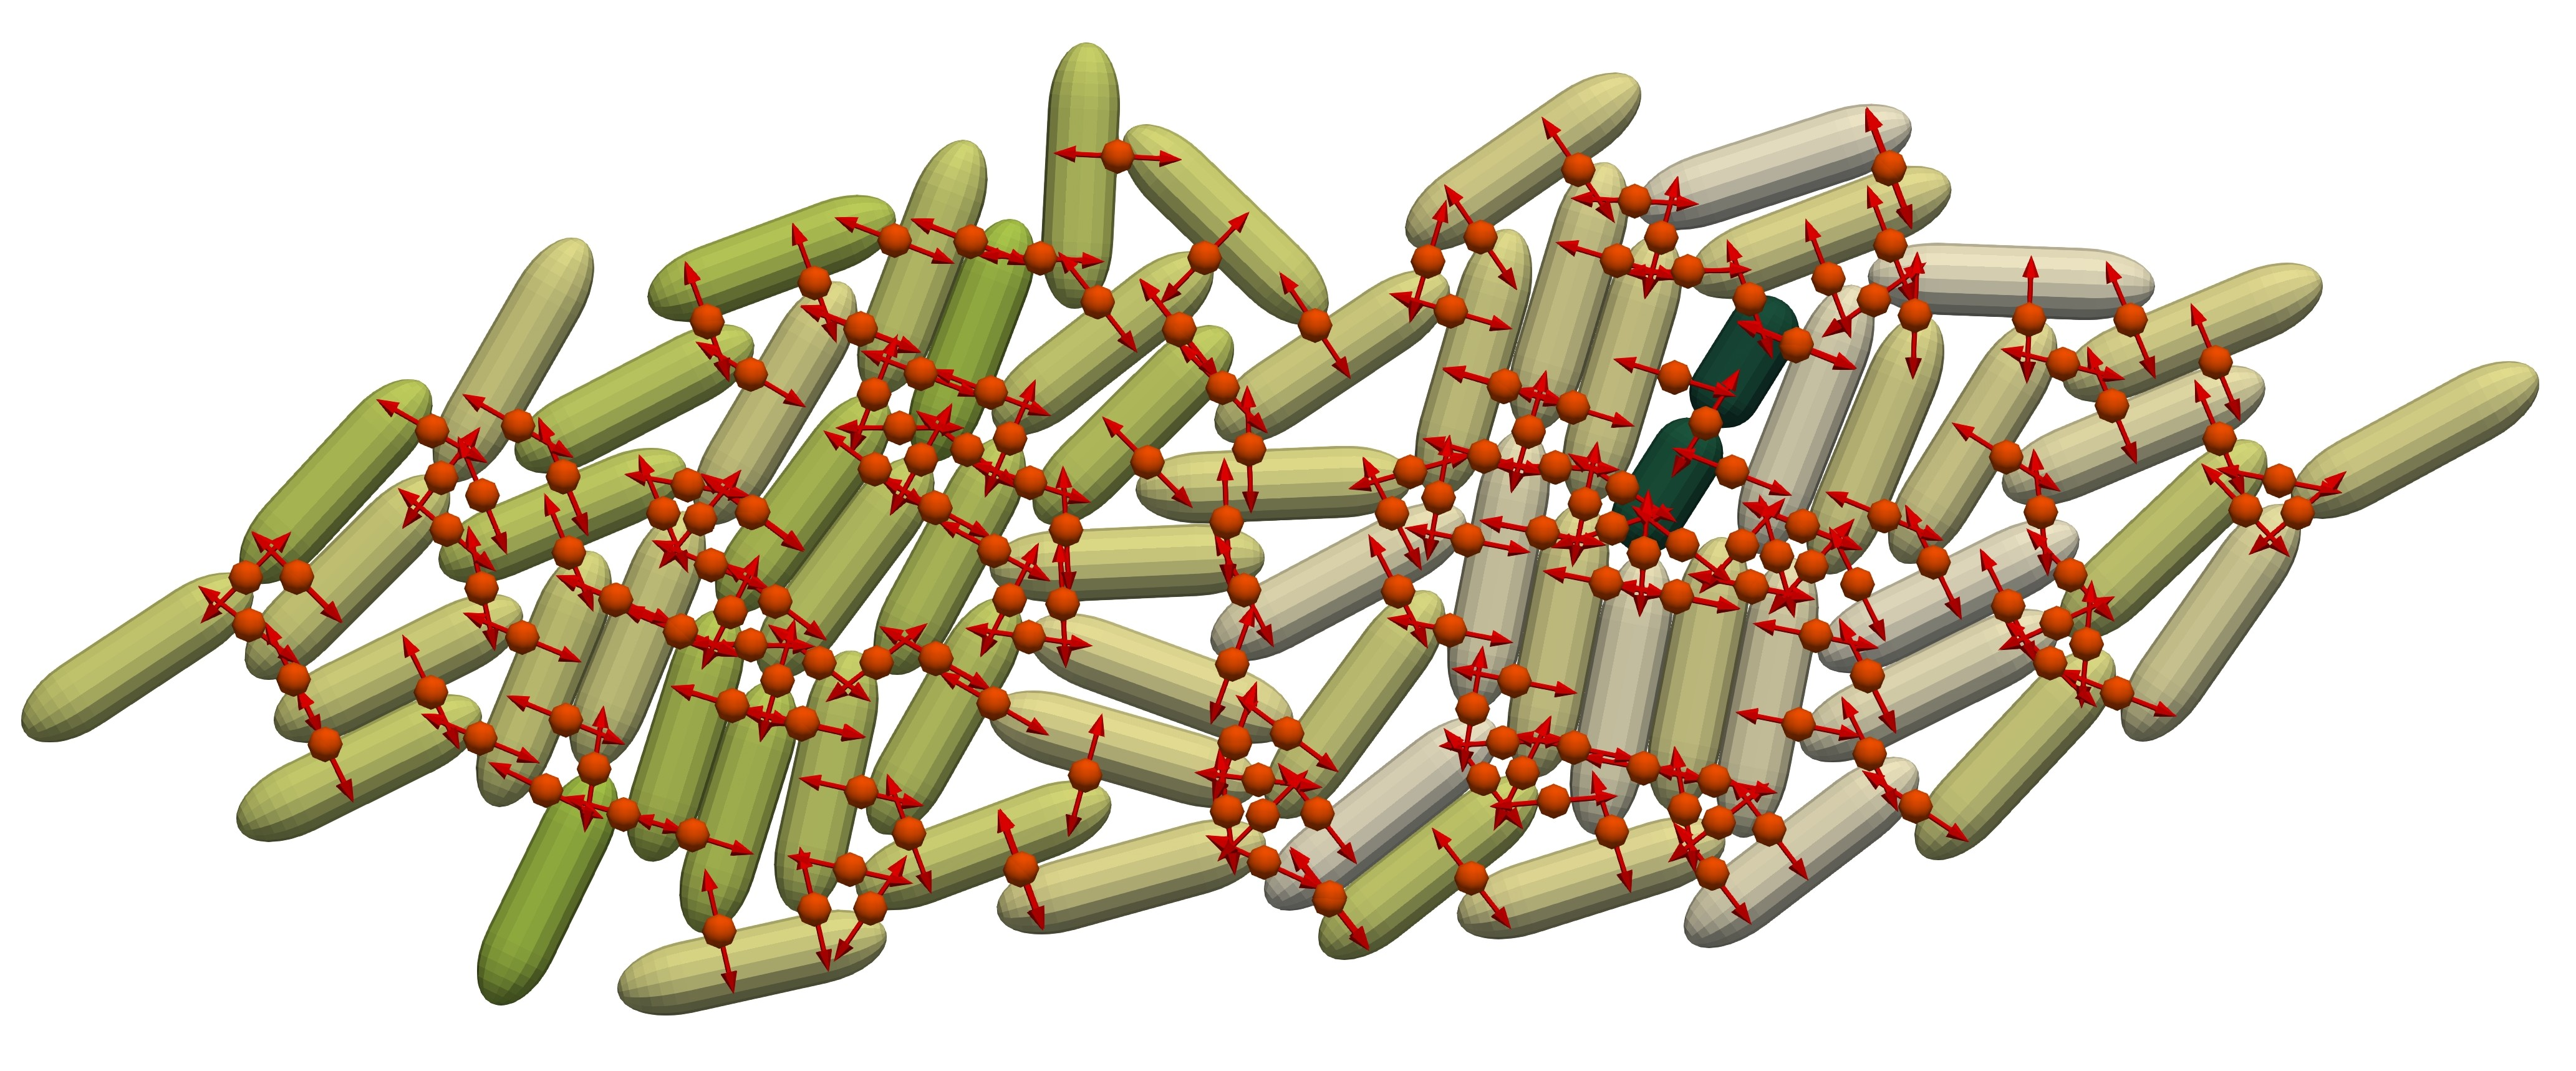
\includegraphics[width=1\textwidth]{figures/constraints.jpeg}
    \end{figure}


    \begin{itemize}
        \item Models only differ in how they calculate force multipliers.
    \end{itemize}

\end{frame}


\begin{frame}
    \frametitle{Soft Model: Hertzian Contact}

    \begin{columns}
        \begin{column}{0.5\textwidth}
            \begin{equation*}
                \mathbf{F}_{ij} = k_{cc} \sqrt{d} \, \delta^{3/2} \, \hat{\mathbf{n}}
            \end{equation*}

            \vspace{0.3cm}

            \textbf{Characteristics:}
            \begin{itemize}
                \item[$+$] Embarrassingly parallel
                \item[$+$] Simple implementation
                \item[$+$] Local calculations
                \item[$-$] Numerically stiff
                \item[$-$] Tiny timesteps ($10^{-5}$)
                \item[$-$] Allows overlap
            \end{itemize}
        \end{column}

        \begin{column}{0.5\textwidth}
            \begin{figure}
                \centering
                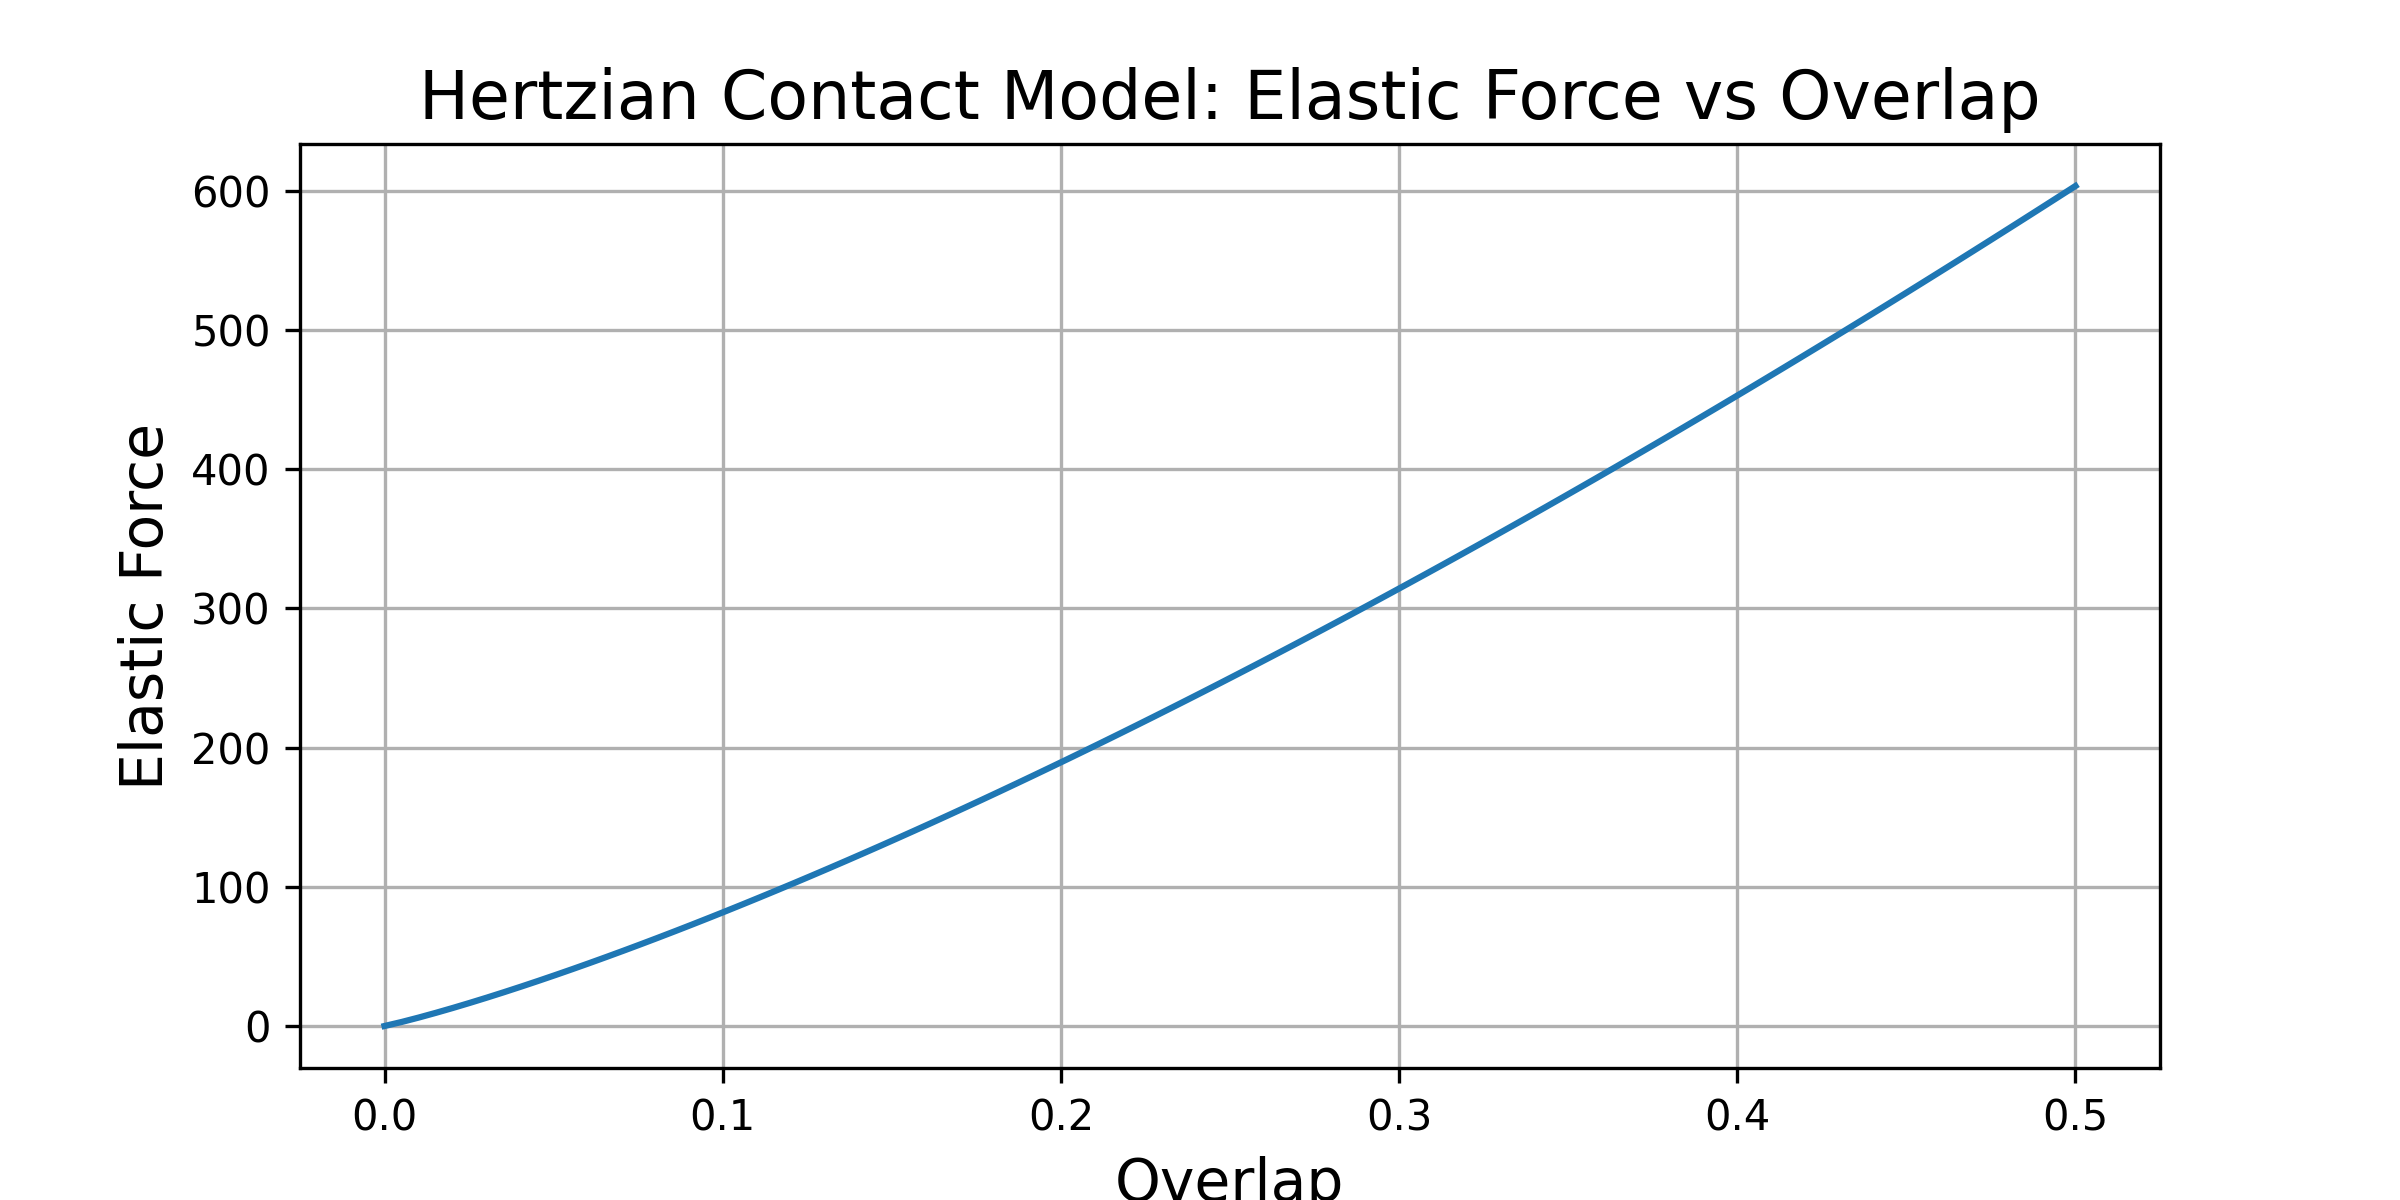
\includegraphics[width=\textwidth]{figures/figures_paper/hertzian_contact_model.png}
                \caption*{\scriptsize{Force increases with overlap}}
            \end{figure}
        \end{column}
    \end{columns}

\end{frame}

\begin{frame}
    \frametitle{Hard Model: Constraint Framework}

    \textbf{Key idea: Introduce non-overlap constraints}
    \begin{itemize}
        \item Define gap function for each contact $c$:
              \begin{equation*}
                  \boldsymbol{\Phi}^k_c = \text{"signed distance at contact } c \text{ at time } k  \text{"}
              \end{equation*}

        \item Express forces based on lagrange multipliers $\boldsymbol{\gamma}$:
              \begin{itemize}
                  \item Contact: $\mathbfcal{F}(\boldsymbol{\gamma}) = \mathbfcal{D} \boldsymbol{\gamma}$
                  \item Stress: $\boldsymbol{\sigma}(\boldsymbol{\gamma}) = \mathbfcal{L} \boldsymbol{\gamma}$
              \end{itemize}
    \end{itemize}

    \vspace{0.3cm}

    \textbf{Physical requirements:}
    \begin{enumerate}
        \item {Repulsive Forces:} \hspace{2.42cm}  $\boldsymbol{\gamma} \geq \mathbf{0}$
        \item {No overlap in next step:} \hspace{1cm} $\boldsymbol{\Phi}^{k+1} \geq \mathbf{0}$
        \item {No force at distance:} \hspace{1cm} $\boldsymbol{\gamma}^\top \boldsymbol{\Phi}^{k+1} = 0$
    \end{enumerate}

\end{frame}


\begin{frame}
    \frametitle{Hard Model: Mathematical Formulation}

    \textbf{Update equations with constraints:}
    \begin{equation} \label{eq:colony_update_with_constraints}
        \begin{split}
            \mathbfcal{C}^{k+1} & = \mathbfcal{C}^k + \Delta t \mathbfcal{G}^k \mathbfcal{M}^k \mathbfcal{F}(\boldsymbol{\gamma})  \\
            \boldsymbol{\ell}^{k+1} & = \boldsymbol{\ell}^k + \Delta t \, \dot{\boldsymbol{\ell}}(\boldsymbol{\gamma}) \\
            \text{s.t.} \quad & \mathbf{0} \leq \boldsymbol{\gamma} \perp \boldsymbol{\Phi}^{k+1}(\boldsymbol{\gamma}) \geq \mathbf{0}.
        \end{split}
    \end{equation}

    \textbf{Reformulate as energy minimization:}
    \begin{equation*} \label{eq:energy_function}
        \min_{\boldsymbol{\gamma} \geq \mathbf{0}}
        E(\boldsymbol{\gamma})
        = \min_{\boldsymbol{\gamma} \geq \mathbf{0}} \boldsymbol{\gamma}^\top \boldsymbol{\Phi}^k
        +  \frac{\Delta t}{2}\, \boldsymbol{\gamma}^\top \mathbfcal{D}^\top \mathbfcal{M}^k \mathbfcal{D}\, \boldsymbol{\gamma}
        + \mathbf{1}^\top \frac{\Delta t}{\lambda}
        \left( \frac{\boldsymbol{\ell}}{\tau} \odot e^{-\lambda\, \mathbfcal{L}\, \boldsymbol{\gamma}} \right)
    \end{equation*}

    \vspace{0.3cm}

    \textbf{Solve via convex optimization:}
    \begin{itemize}
        \item Solve for $\boldsymbol{\gamma}^{*}$ that minimizes $E(\boldsymbol{\gamma}^{*} )$
        \item Guarantees satisfaction of all constraints
        \item (See Paper for derivation)
    \end{itemize}


\end{frame}

\begin{frame}
    \frametitle{Hard Model: Solver Pipeline}

    \begin{enumerate}
        \item \textbf{BBPGD Solver:} Projected gradient descent
              \begin{itemize}
                  \item Iteratively minimize $E(\boldsymbol{\gamma})$
                  \item Typically $\sim$2500 iterations
                  \item Converges to tolerance $\epsilon = 10^{-3}$
              \end{itemize}

              \vspace{0.3cm}

        \item \textbf{ReLCP Refinement:} Remove residual overlaps
              \begin{itemize}
                  \item Detect remaining violations
                  \item Add new constraints
                  \item Re-solve (typically 6 iterations)
              \end{itemize}
    \end{enumerate}

    \vspace{0.5cm}

    \textbf{Characteristics:}
    \begin{itemize}
        \item[$+$] Larger timesteps ($3 \cdot 10^{-4}$)
        \item[$+$] Strict non-overlap
        \item[$-$] High per-step cost
        \item[$-$] Complex implementation
    \end{itemize}

\end{frame}

% ============================================================
% SECTION 5: BIOLOGICAL VALIDATION
% ============================================================

\section{Pattern Formation Results}

\begin{frame}
    \frametitle{Concentric Rings: Qualitative Comparison}

    % Suggest: Show side-by-side video comparison here if available
    % \movie[width=0.45\textwidth]{}{hard_growth.mp4} \hfill \movie[width=0.45\textwidth]{}{soft_growth.mp4}


    \vspace{-0.3cm}
    \begin{figure}
        \centering
        \begin{tabular}{r M{0.25\textwidth} M{0.25\textwidth} M{0.25\textwidth}}
                                                                                                             & $\lambda = 10^{-4}$   & $\lambda = 10^{-3}$      & $\lambda = 10^{-2}$
            \\[3pt]
            \textbf{Hard}                                                                                    &
            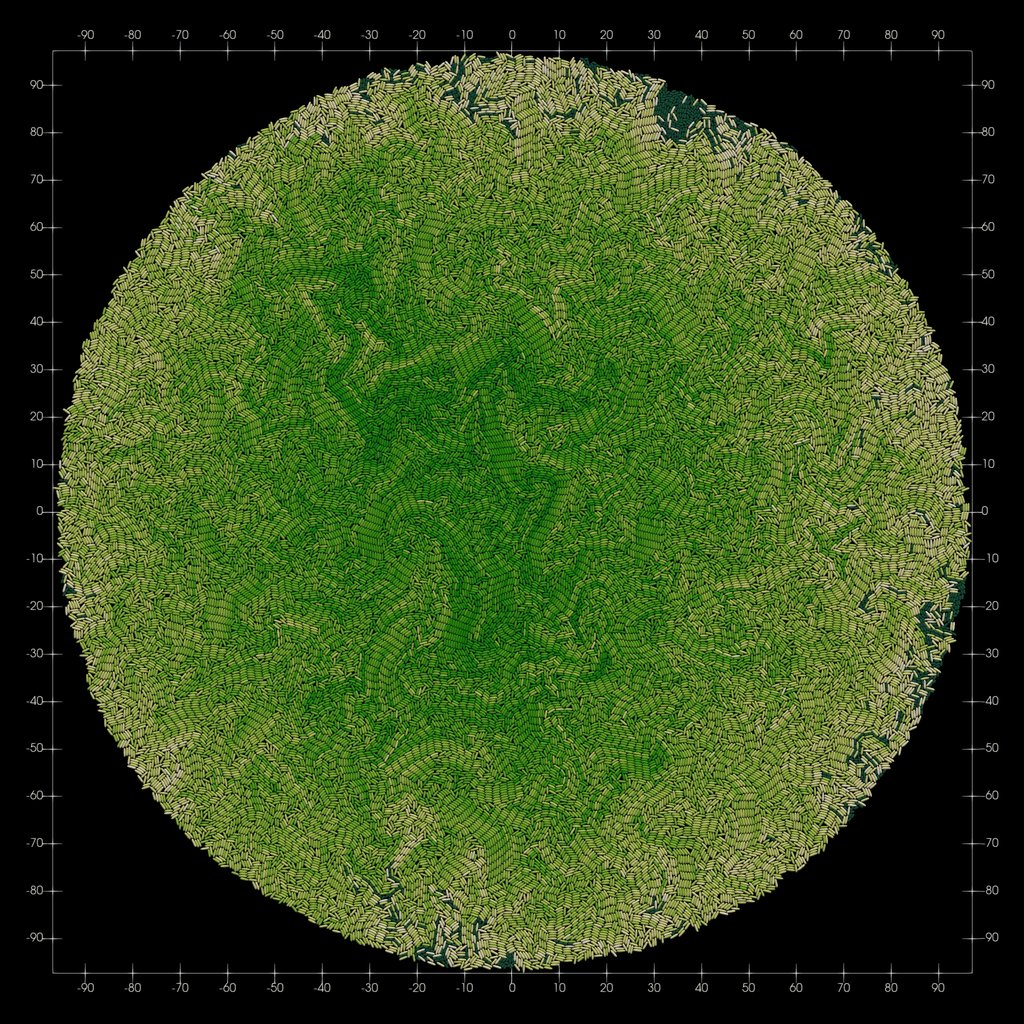
\includegraphics[width=0.25\textwidth]{figures/figures_paper/growth/hard_e-4/hard_e-4.0192.jpeg} &
            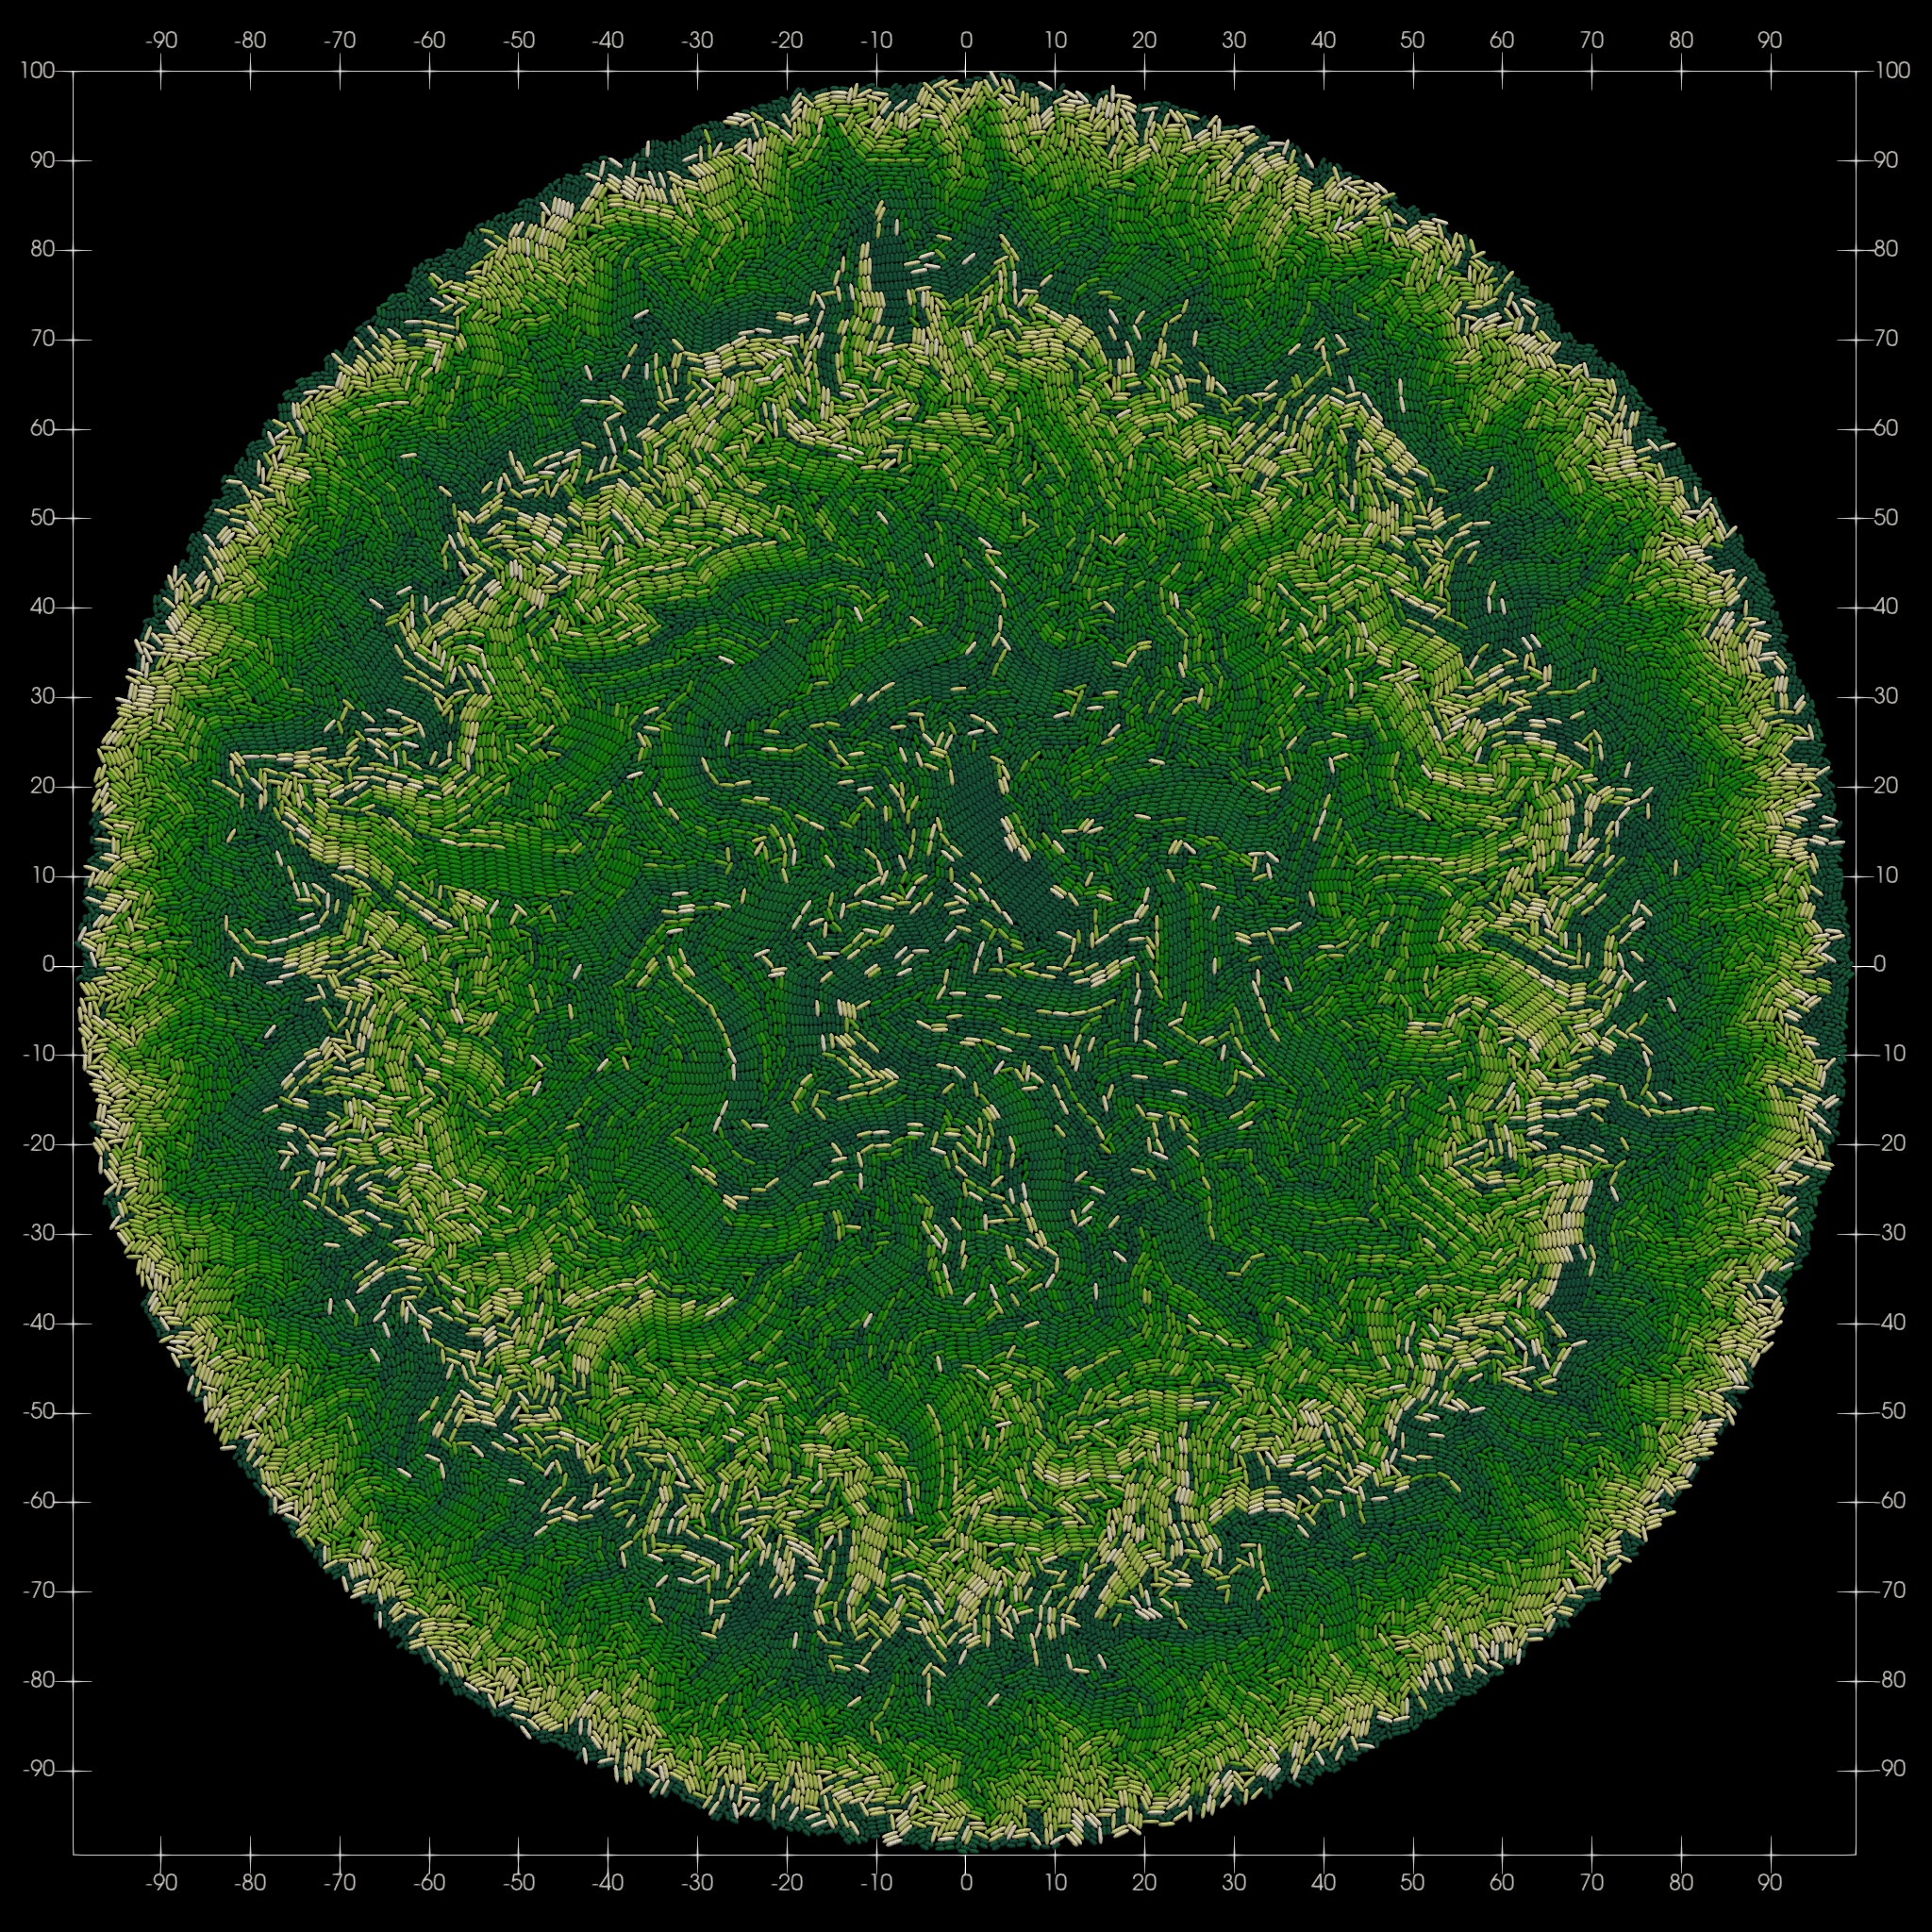
\includegraphics[width=0.25\textwidth]{figures/figures_paper/growth/hard_e-3/hard_e-3.0198.jpeg} &
            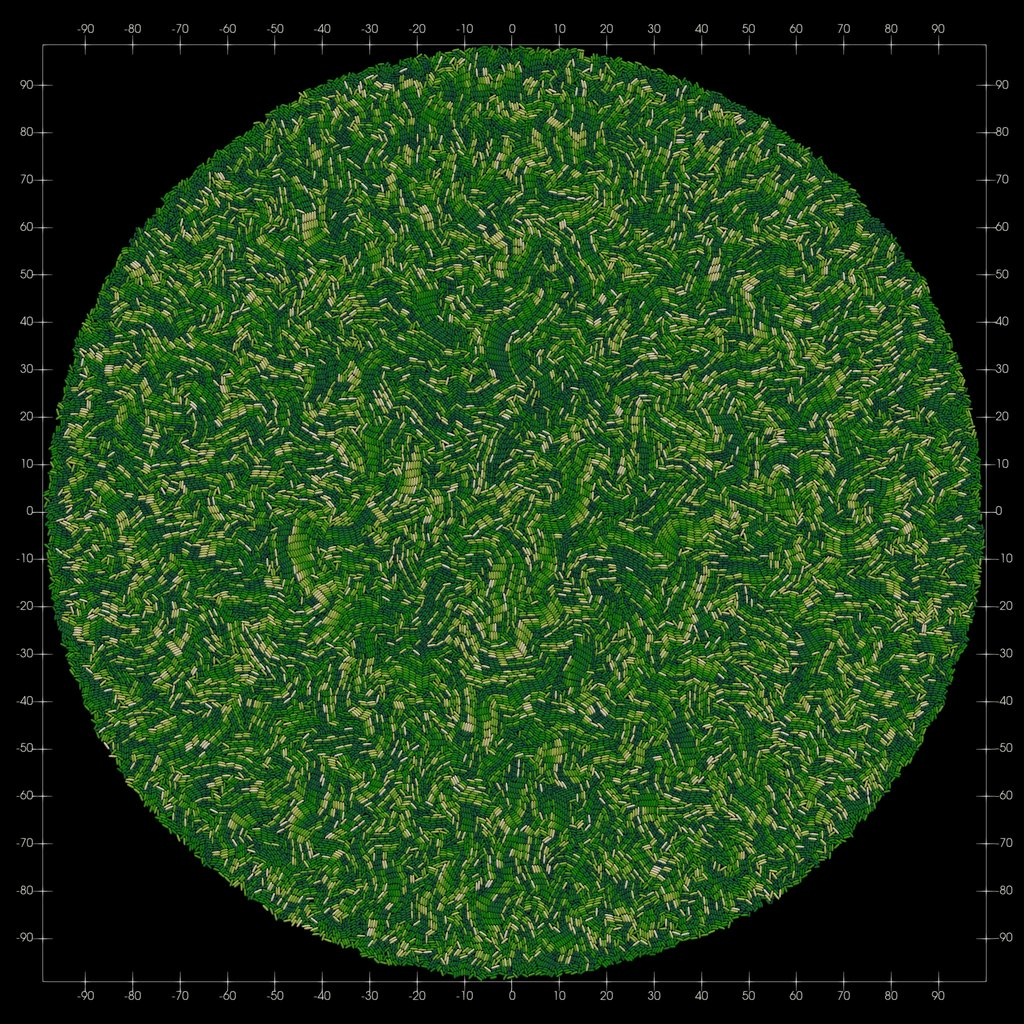
\includegraphics[width=0.25\textwidth]{figures/figures_paper/growth/hard_e-2/hard_e-2.0199.jpeg}                                                                               \\[3pt]

            \textbf{Soft}                                                                                    &
            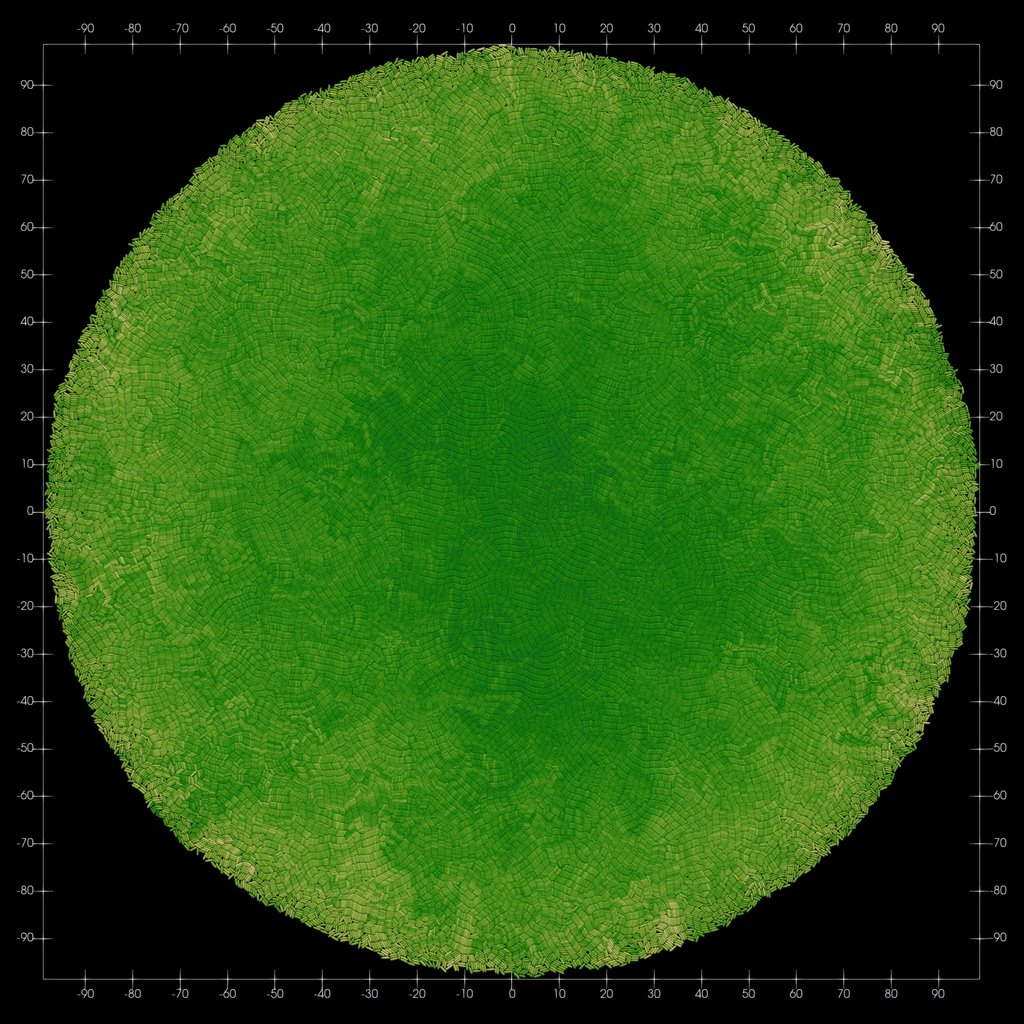
\includegraphics[width=0.25\textwidth]{figures/figures_paper/growth/soft_e-4/soft_e-4.0198.jpeg} &
            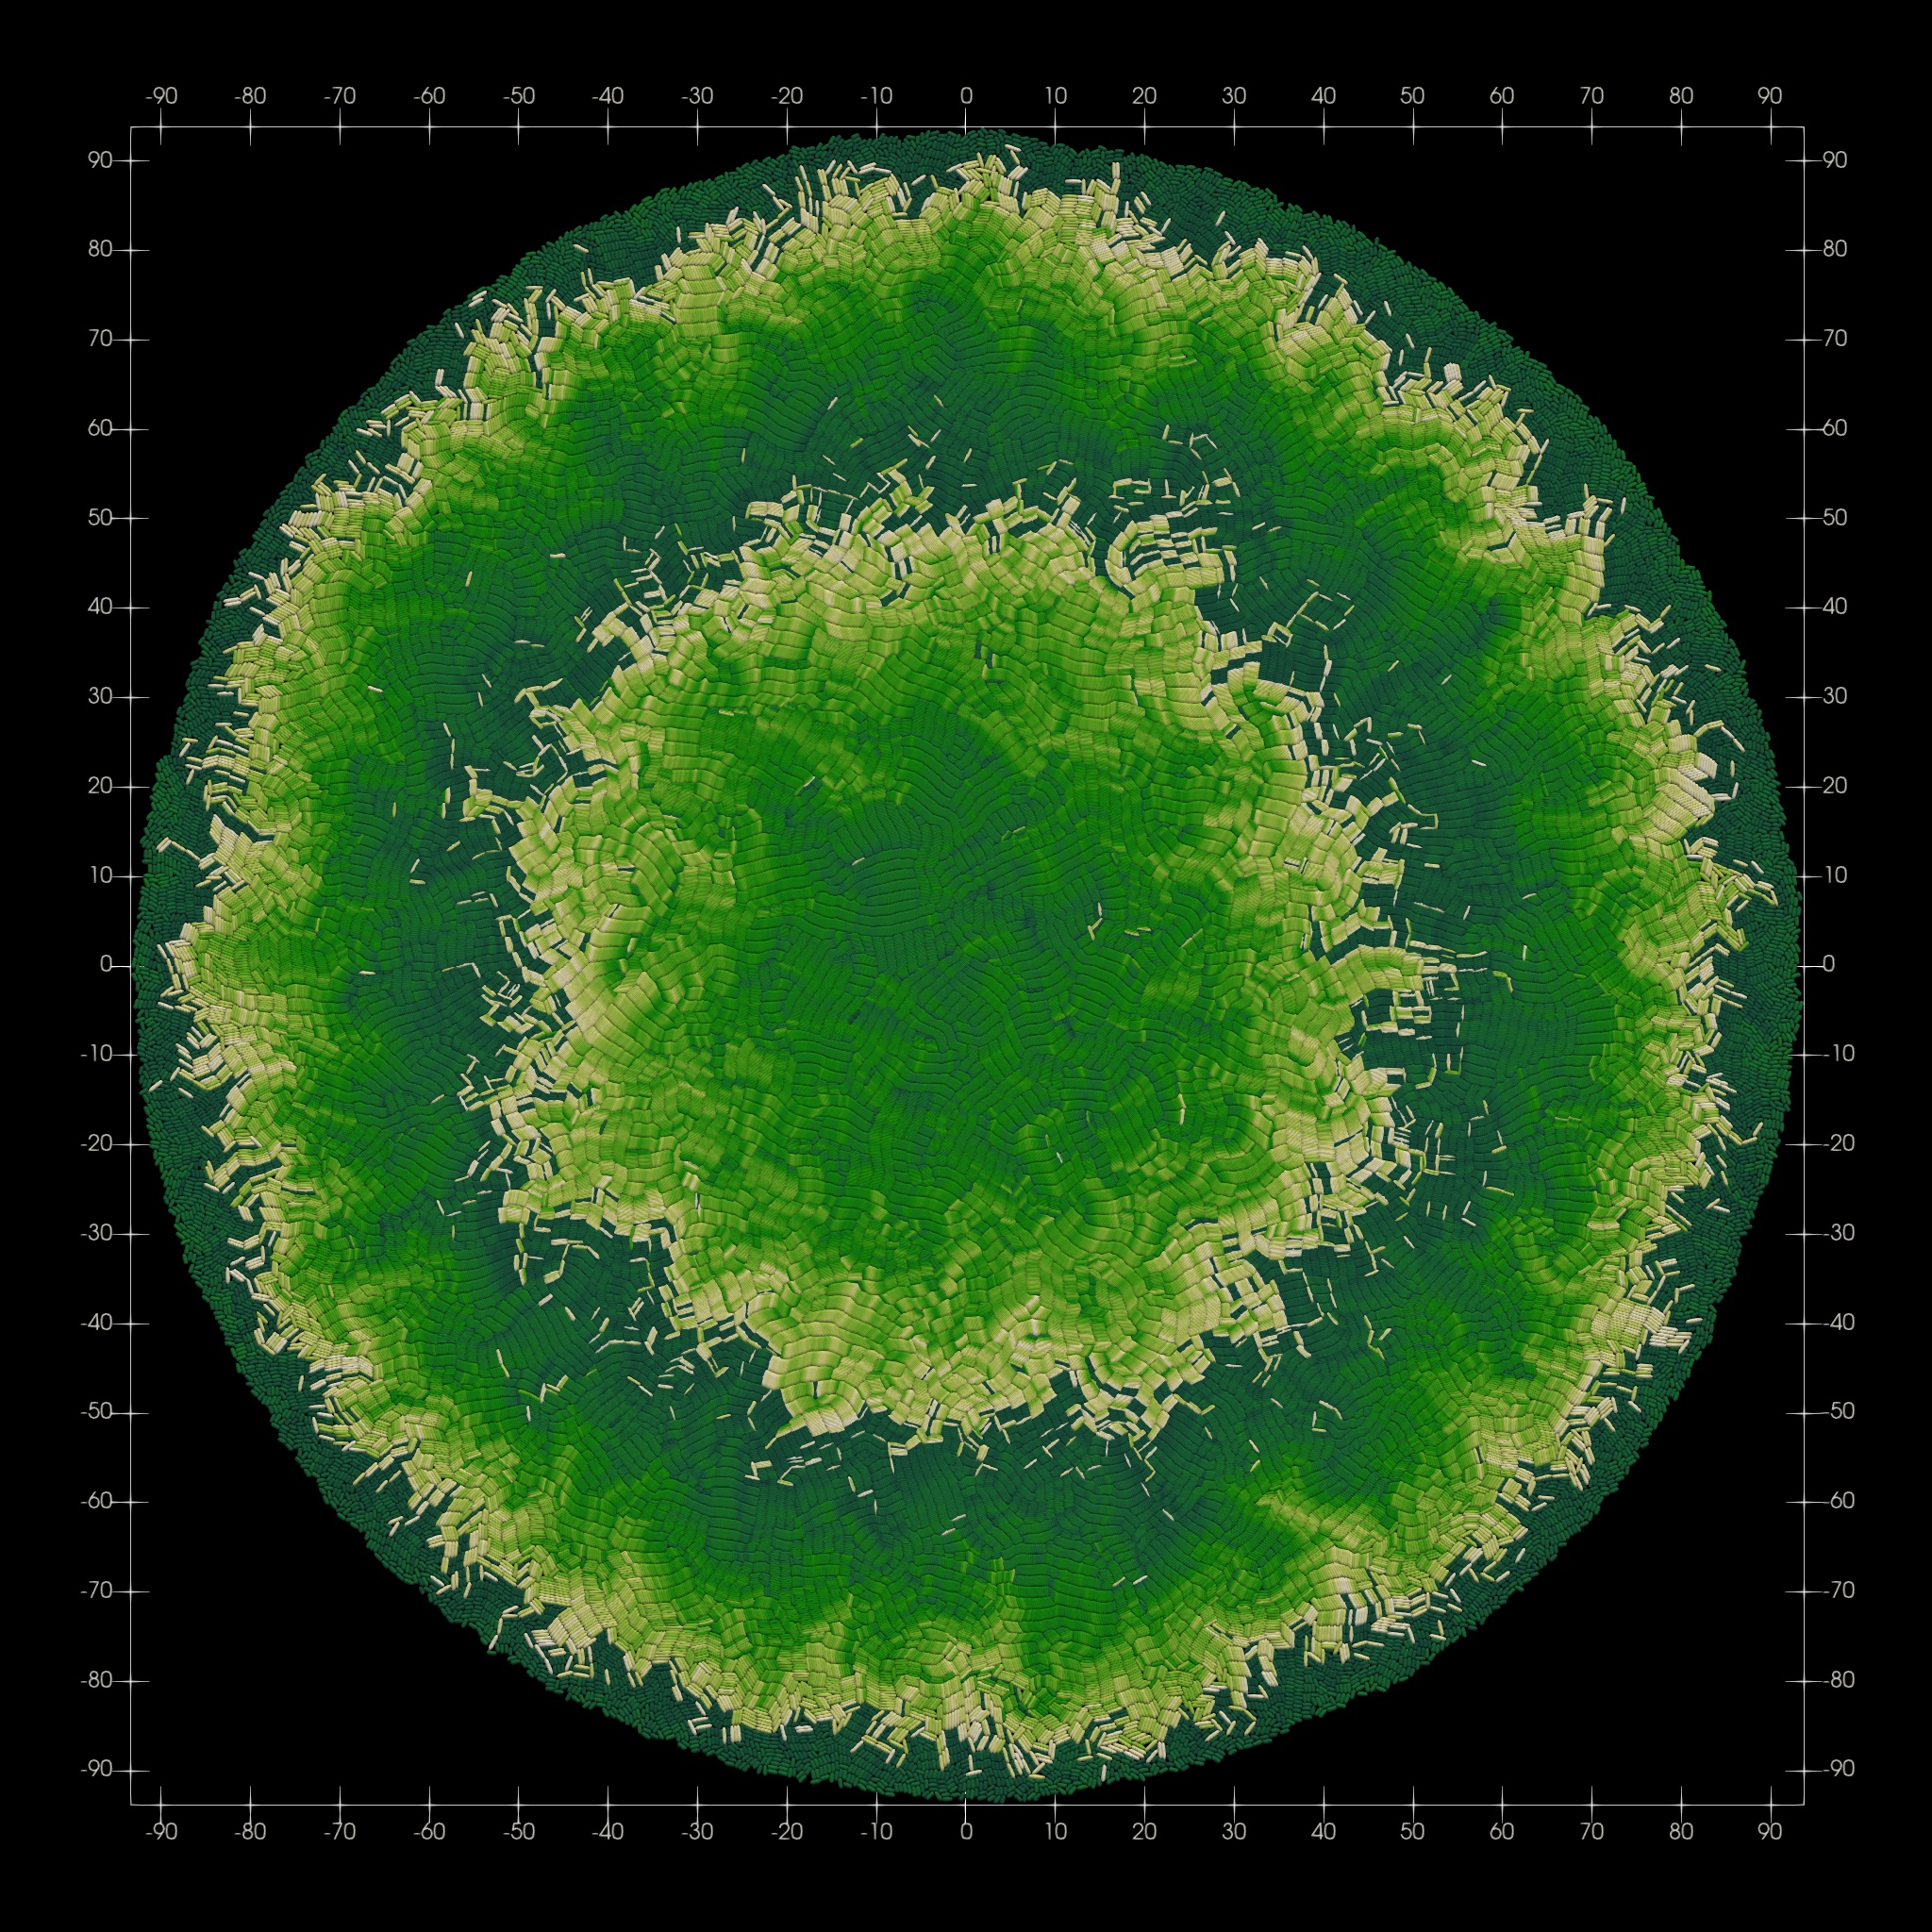
\includegraphics[width=0.25\textwidth]{figures/figures_paper/growth/soft_e-3/soft_e-3.0187.jpeg} &
            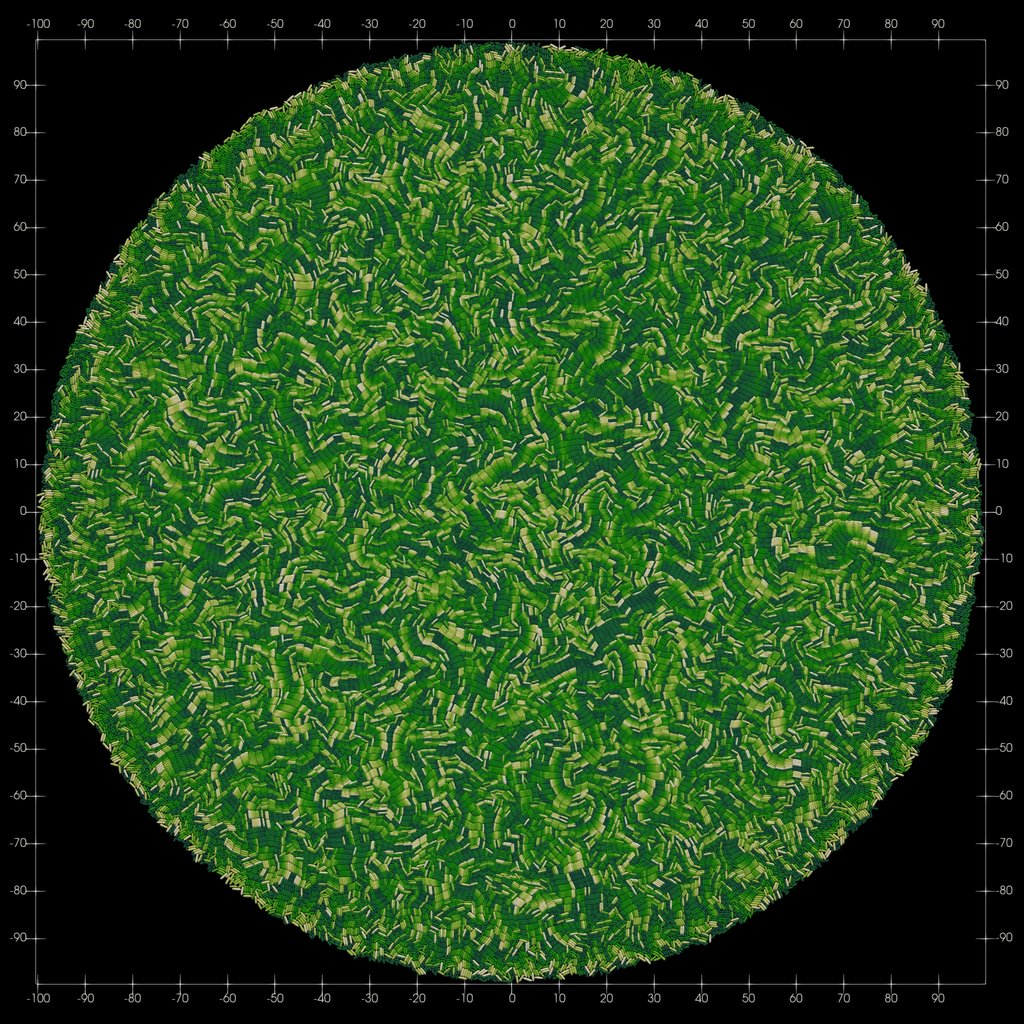
\includegraphics[width=0.25\textwidth]{figures/figures_paper/growth/soft_e-2/soft_e-2.0200.jpeg}                                                                               \\[3pt]

                                                                                                             & \scriptsize{No rings} & \scriptsize{Clear rings} & \scriptsize{Dissipating}
        \end{tabular}
    \end{figure}

\end{frame}

\begin{frame}
    \frametitle{The Critical Difference: Packing Density}

    \begin{columns}
        \begin{column}{0.5\textwidth}
            \begin{figure}
                \centering
                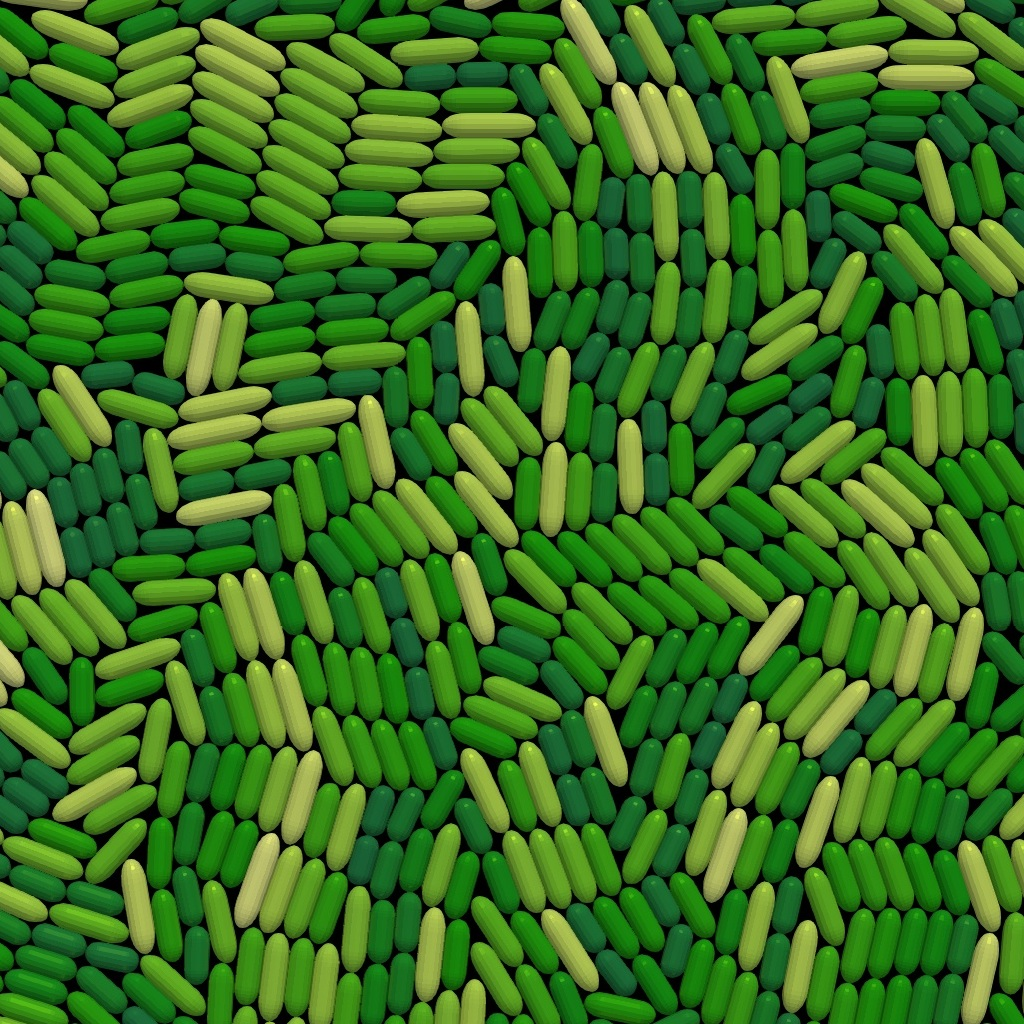
\includegraphics[width=0.9\textwidth]{figures/figures_paper/comparison_plots/density_hard.jpeg}
                \caption*{\textbf{Hard Model}}
            \end{figure}

            \vspace{-0.2cm}

            \begin{itemize}
                \item Packing fraction $\phi \approx 0.9$
                \item Physically realistic
                \item Sharp boundaries
            \end{itemize}
        \end{column}

        \begin{column}{0.5\textwidth}
            \begin{figure}
                \centering
                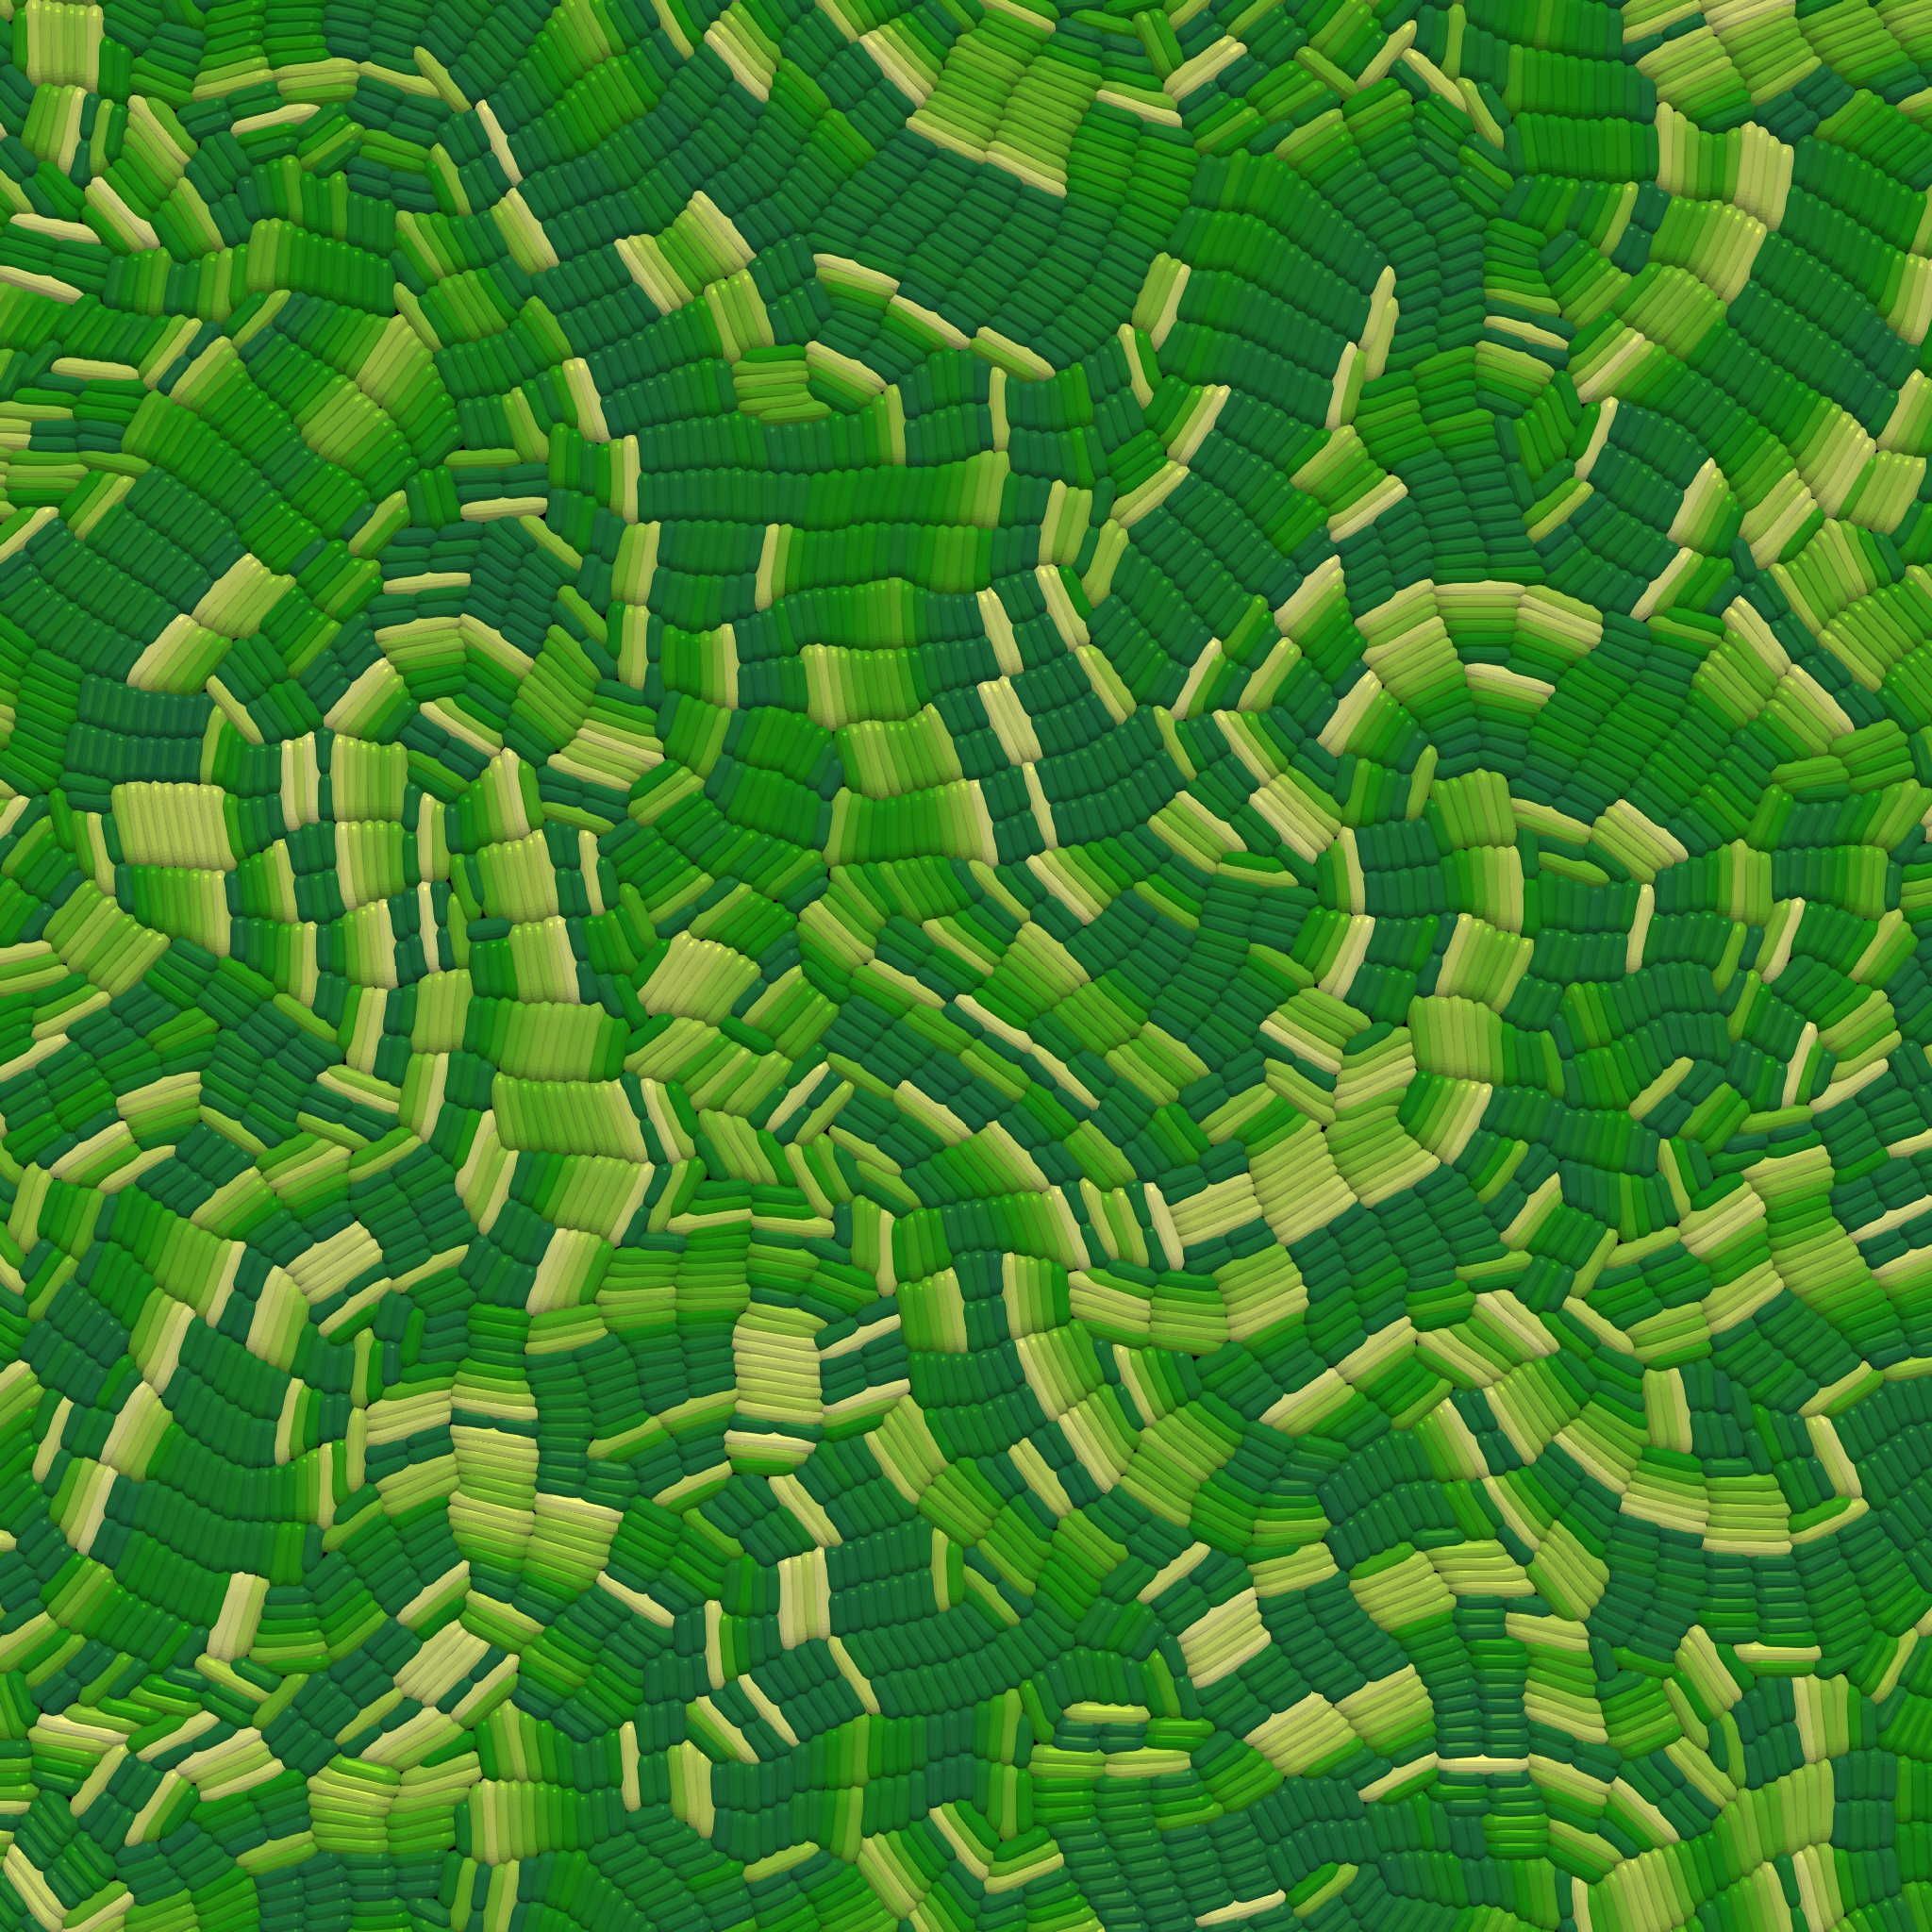
\includegraphics[width=0.9\textwidth]{figures/figures_paper/comparison_plots/density_soft.jpeg}
                \caption*{\textbf{Soft Model}}
            \end{figure}

            \vspace{-0.2cm}

            \begin{itemize}
                \item Packing fraction $\phi > 5$ !
                \item Unphysical overlap
                \item Fuzzy appearance
            \end{itemize}
        \end{column}
    \end{columns}

\end{frame}

\begin{frame}
    \frametitle{Quantifying the Packing Problem}

    \begin{figure}
        \centering
        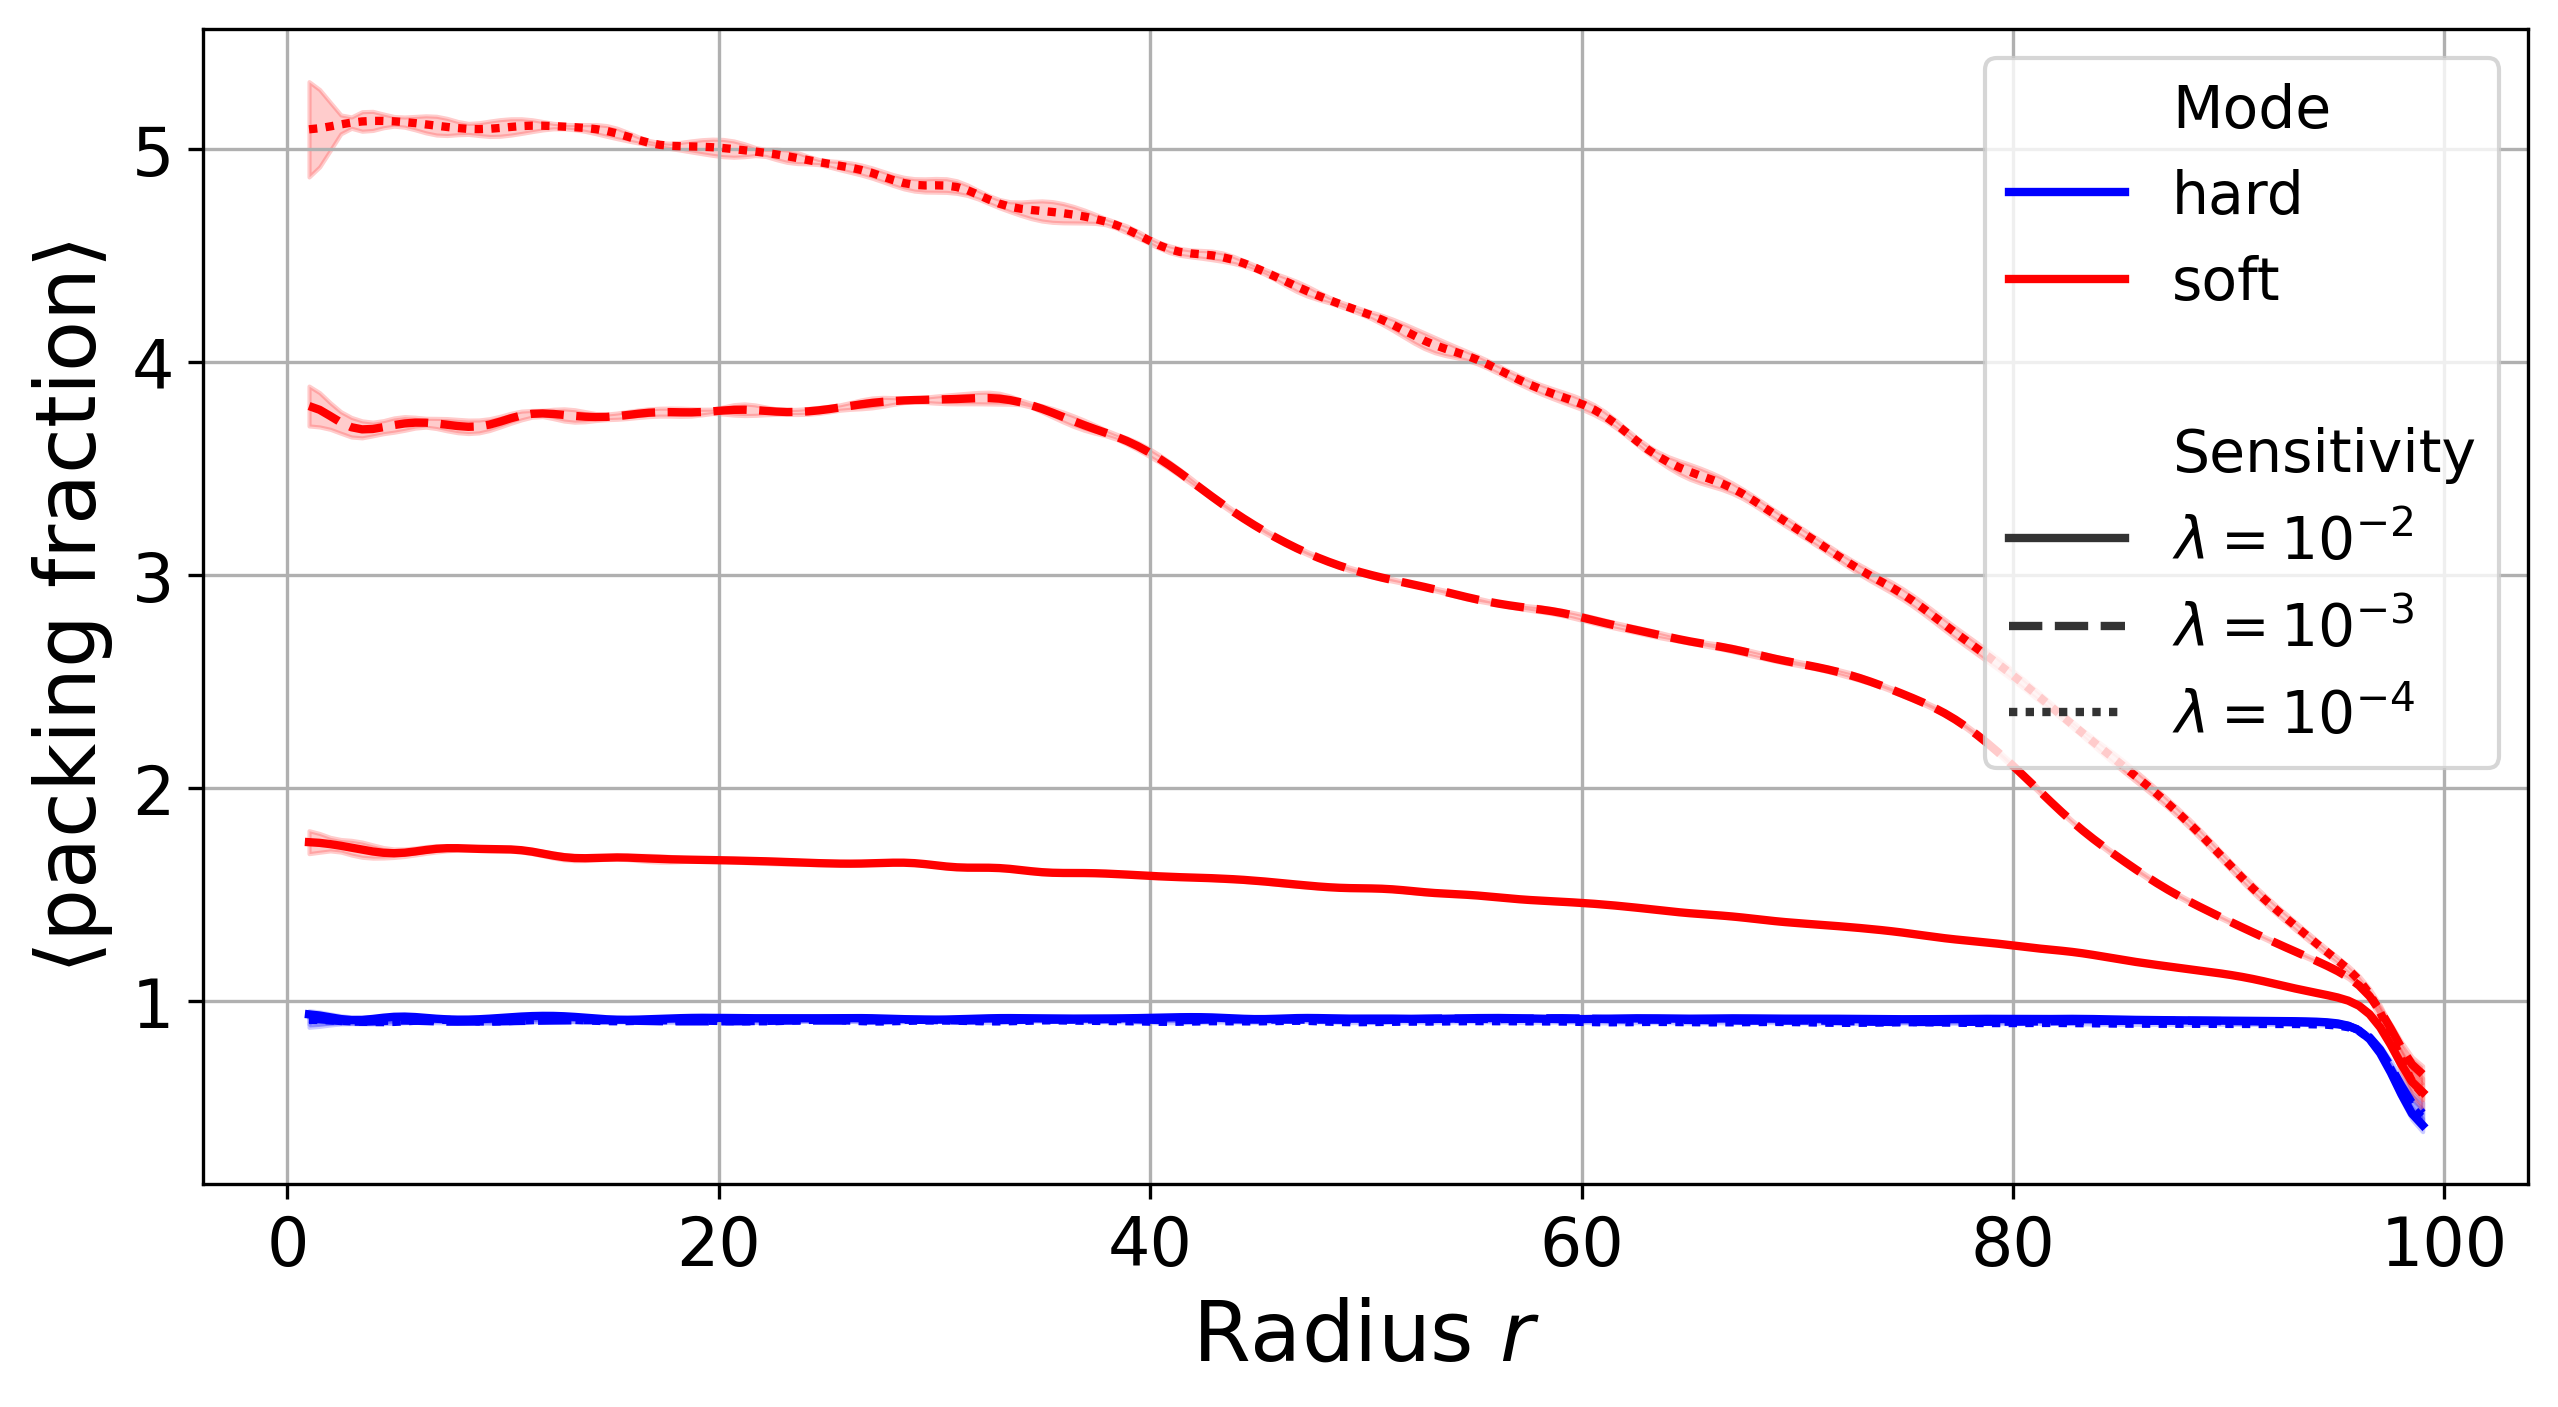
\includegraphics[width=0.8\textwidth]{figures/figures_paper/comparison_plots/combined_radial_packing_fraction.png}
    \end{figure}

    \begin{itemize}
        \item Soft model: extreme center overcrowding
        \item Gets worse at low $\lambda$ (weak inhibition)
        \item Hard model: constant realistic packing
    \end{itemize}

\end{frame}

\begin{frame}
    \frametitle{Microdomain Formation}

    \begin{columns}
        \begin{column}{0.5\textwidth}

            \textbf{Small colonies ($R \approx 50$):}
            \begin{itemize}
                \item Both work well
                \item Similar patch structure
                \item Matches experiments
            \end{itemize}

            \vspace{0.5cm}

            \textbf{Large colonies:}
            \begin{itemize}
                \item Hard: consistent patches
                \item Soft: elongated bundles
                \item Artifact from overcrowding
            \end{itemize}
        \end{column}

        \begin{column}{0.5\textwidth}
            \vspace{-2.3cm}
            \begin{figure}
                \centering
                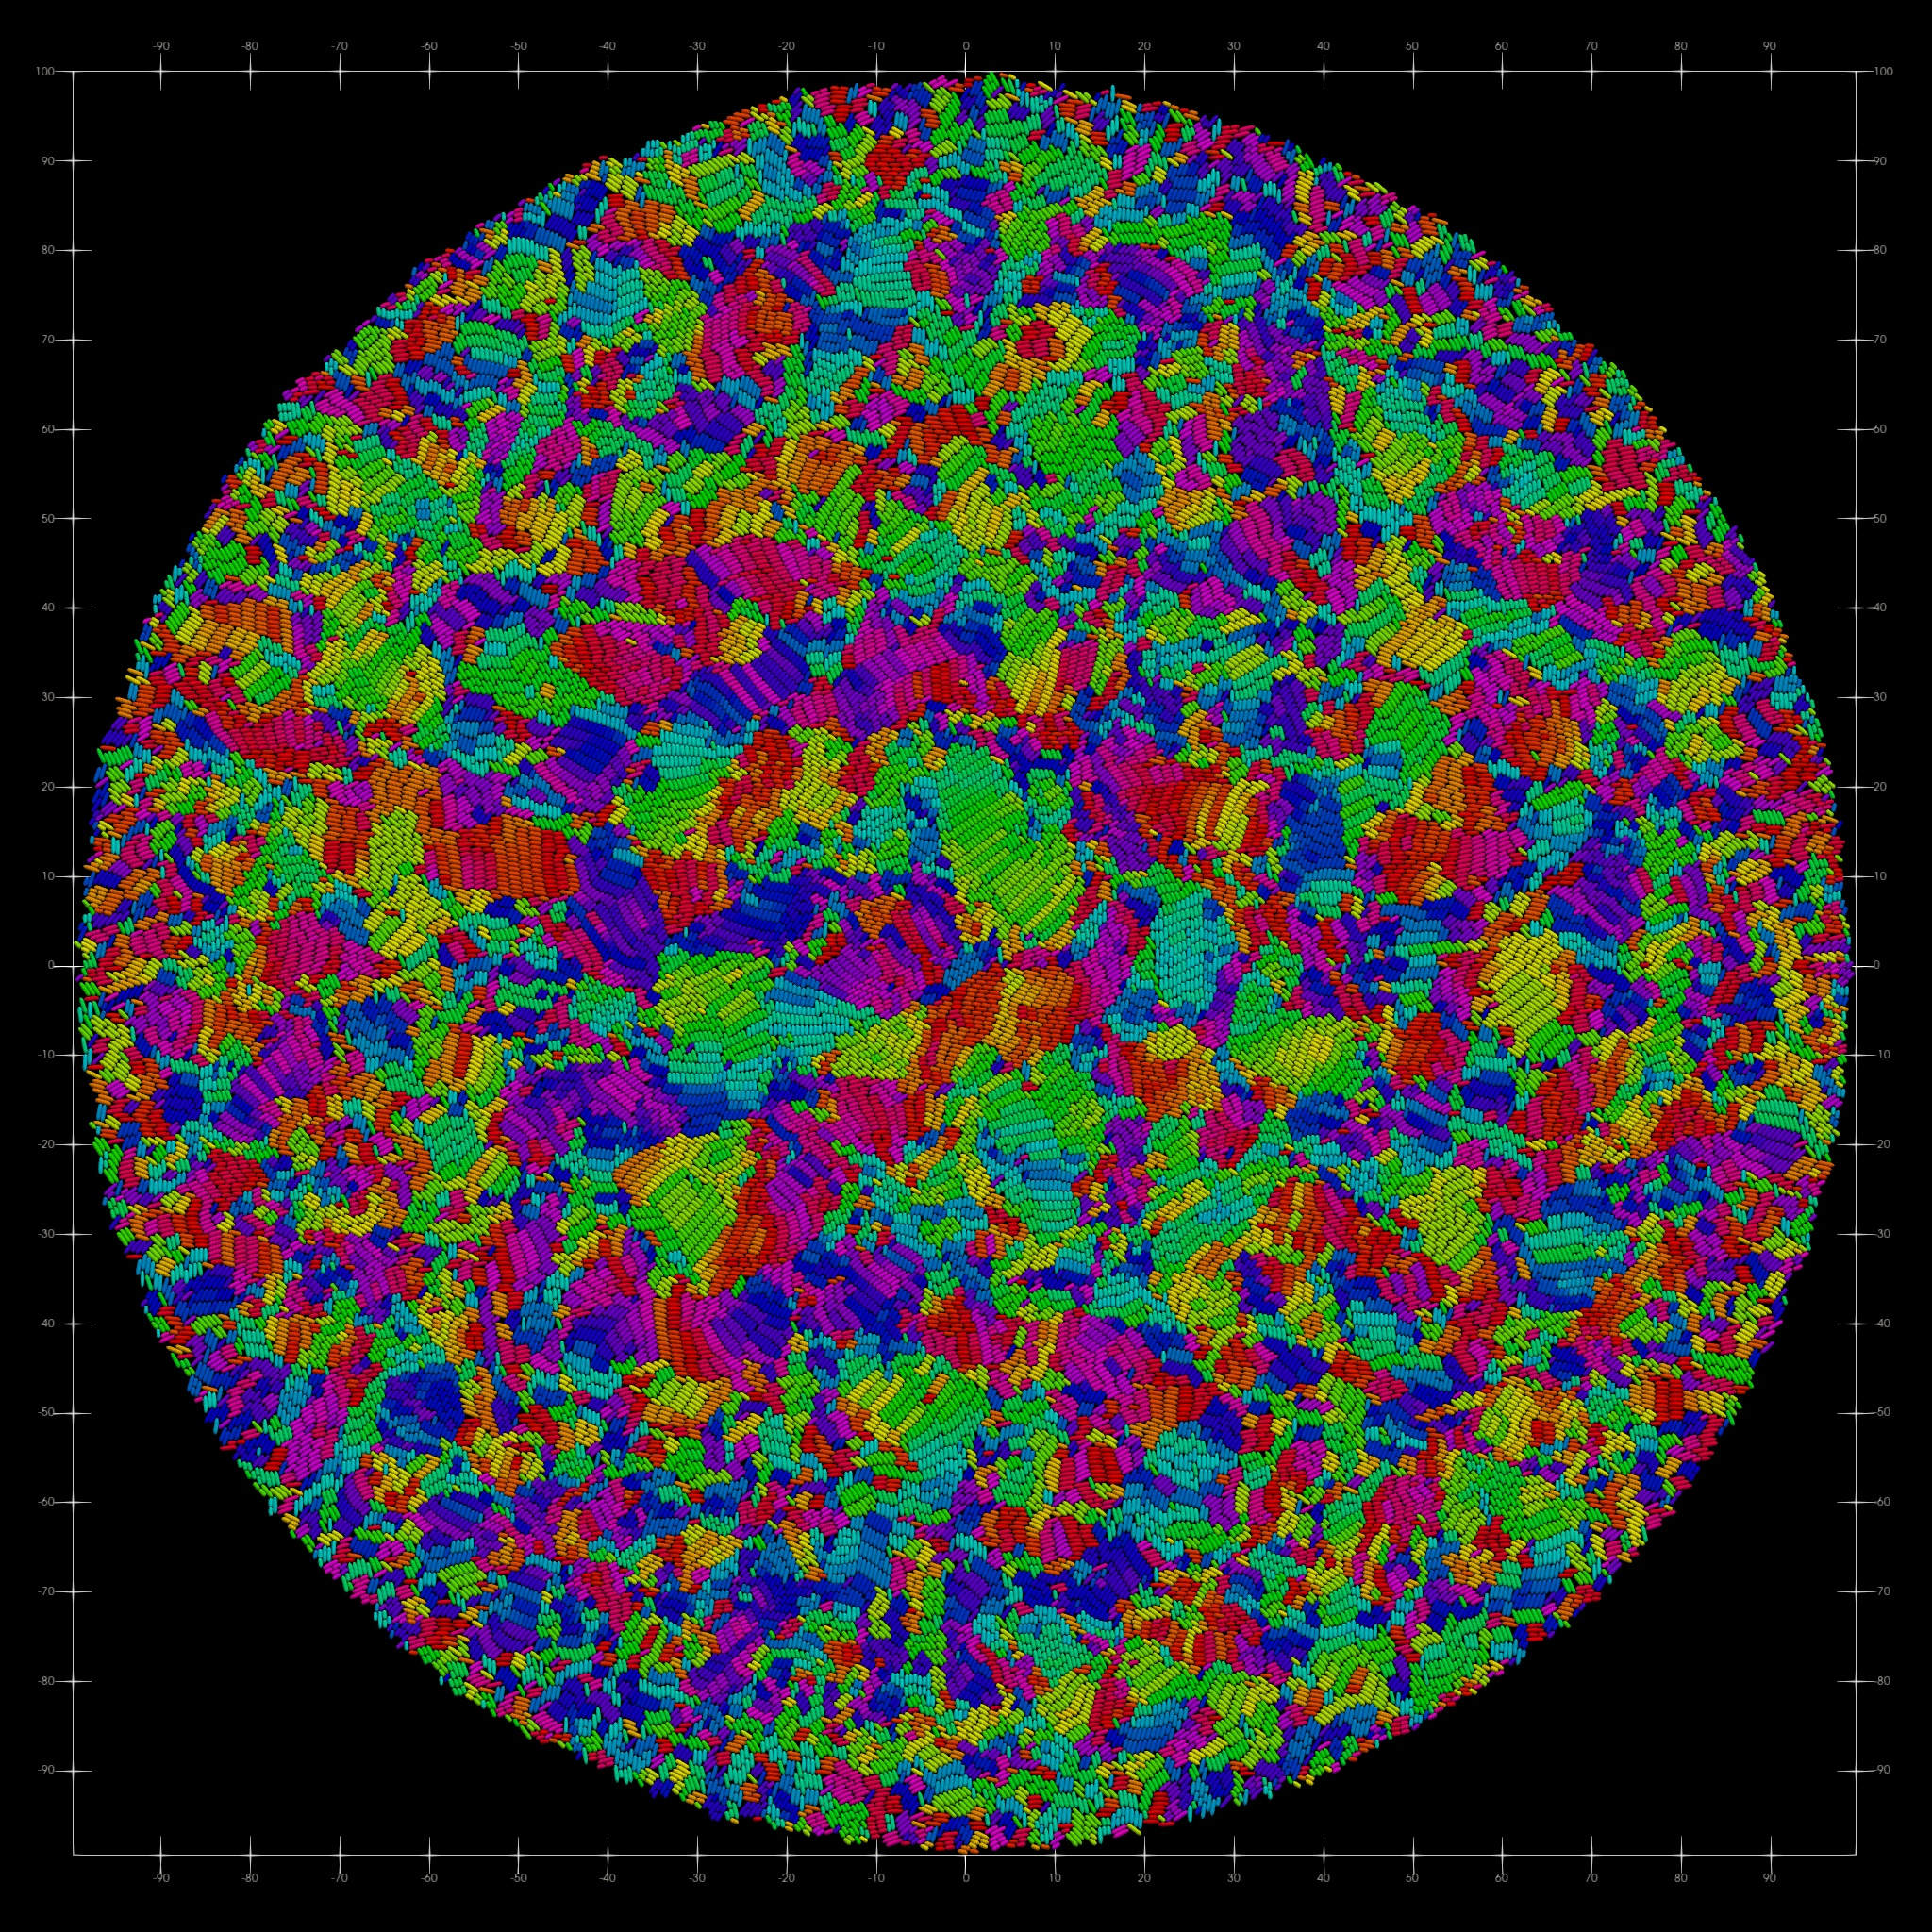
\includegraphics[width=0.62\textwidth]{figures/figures_paper/orientation_comparisons/zoomed_images/hard_e-3_orient.jpeg}
                \caption*{\scriptsize{Hard: realistic patches}}
            \end{figure}
            \vspace{-0.7cm}
            \begin{figure}
                \centering
                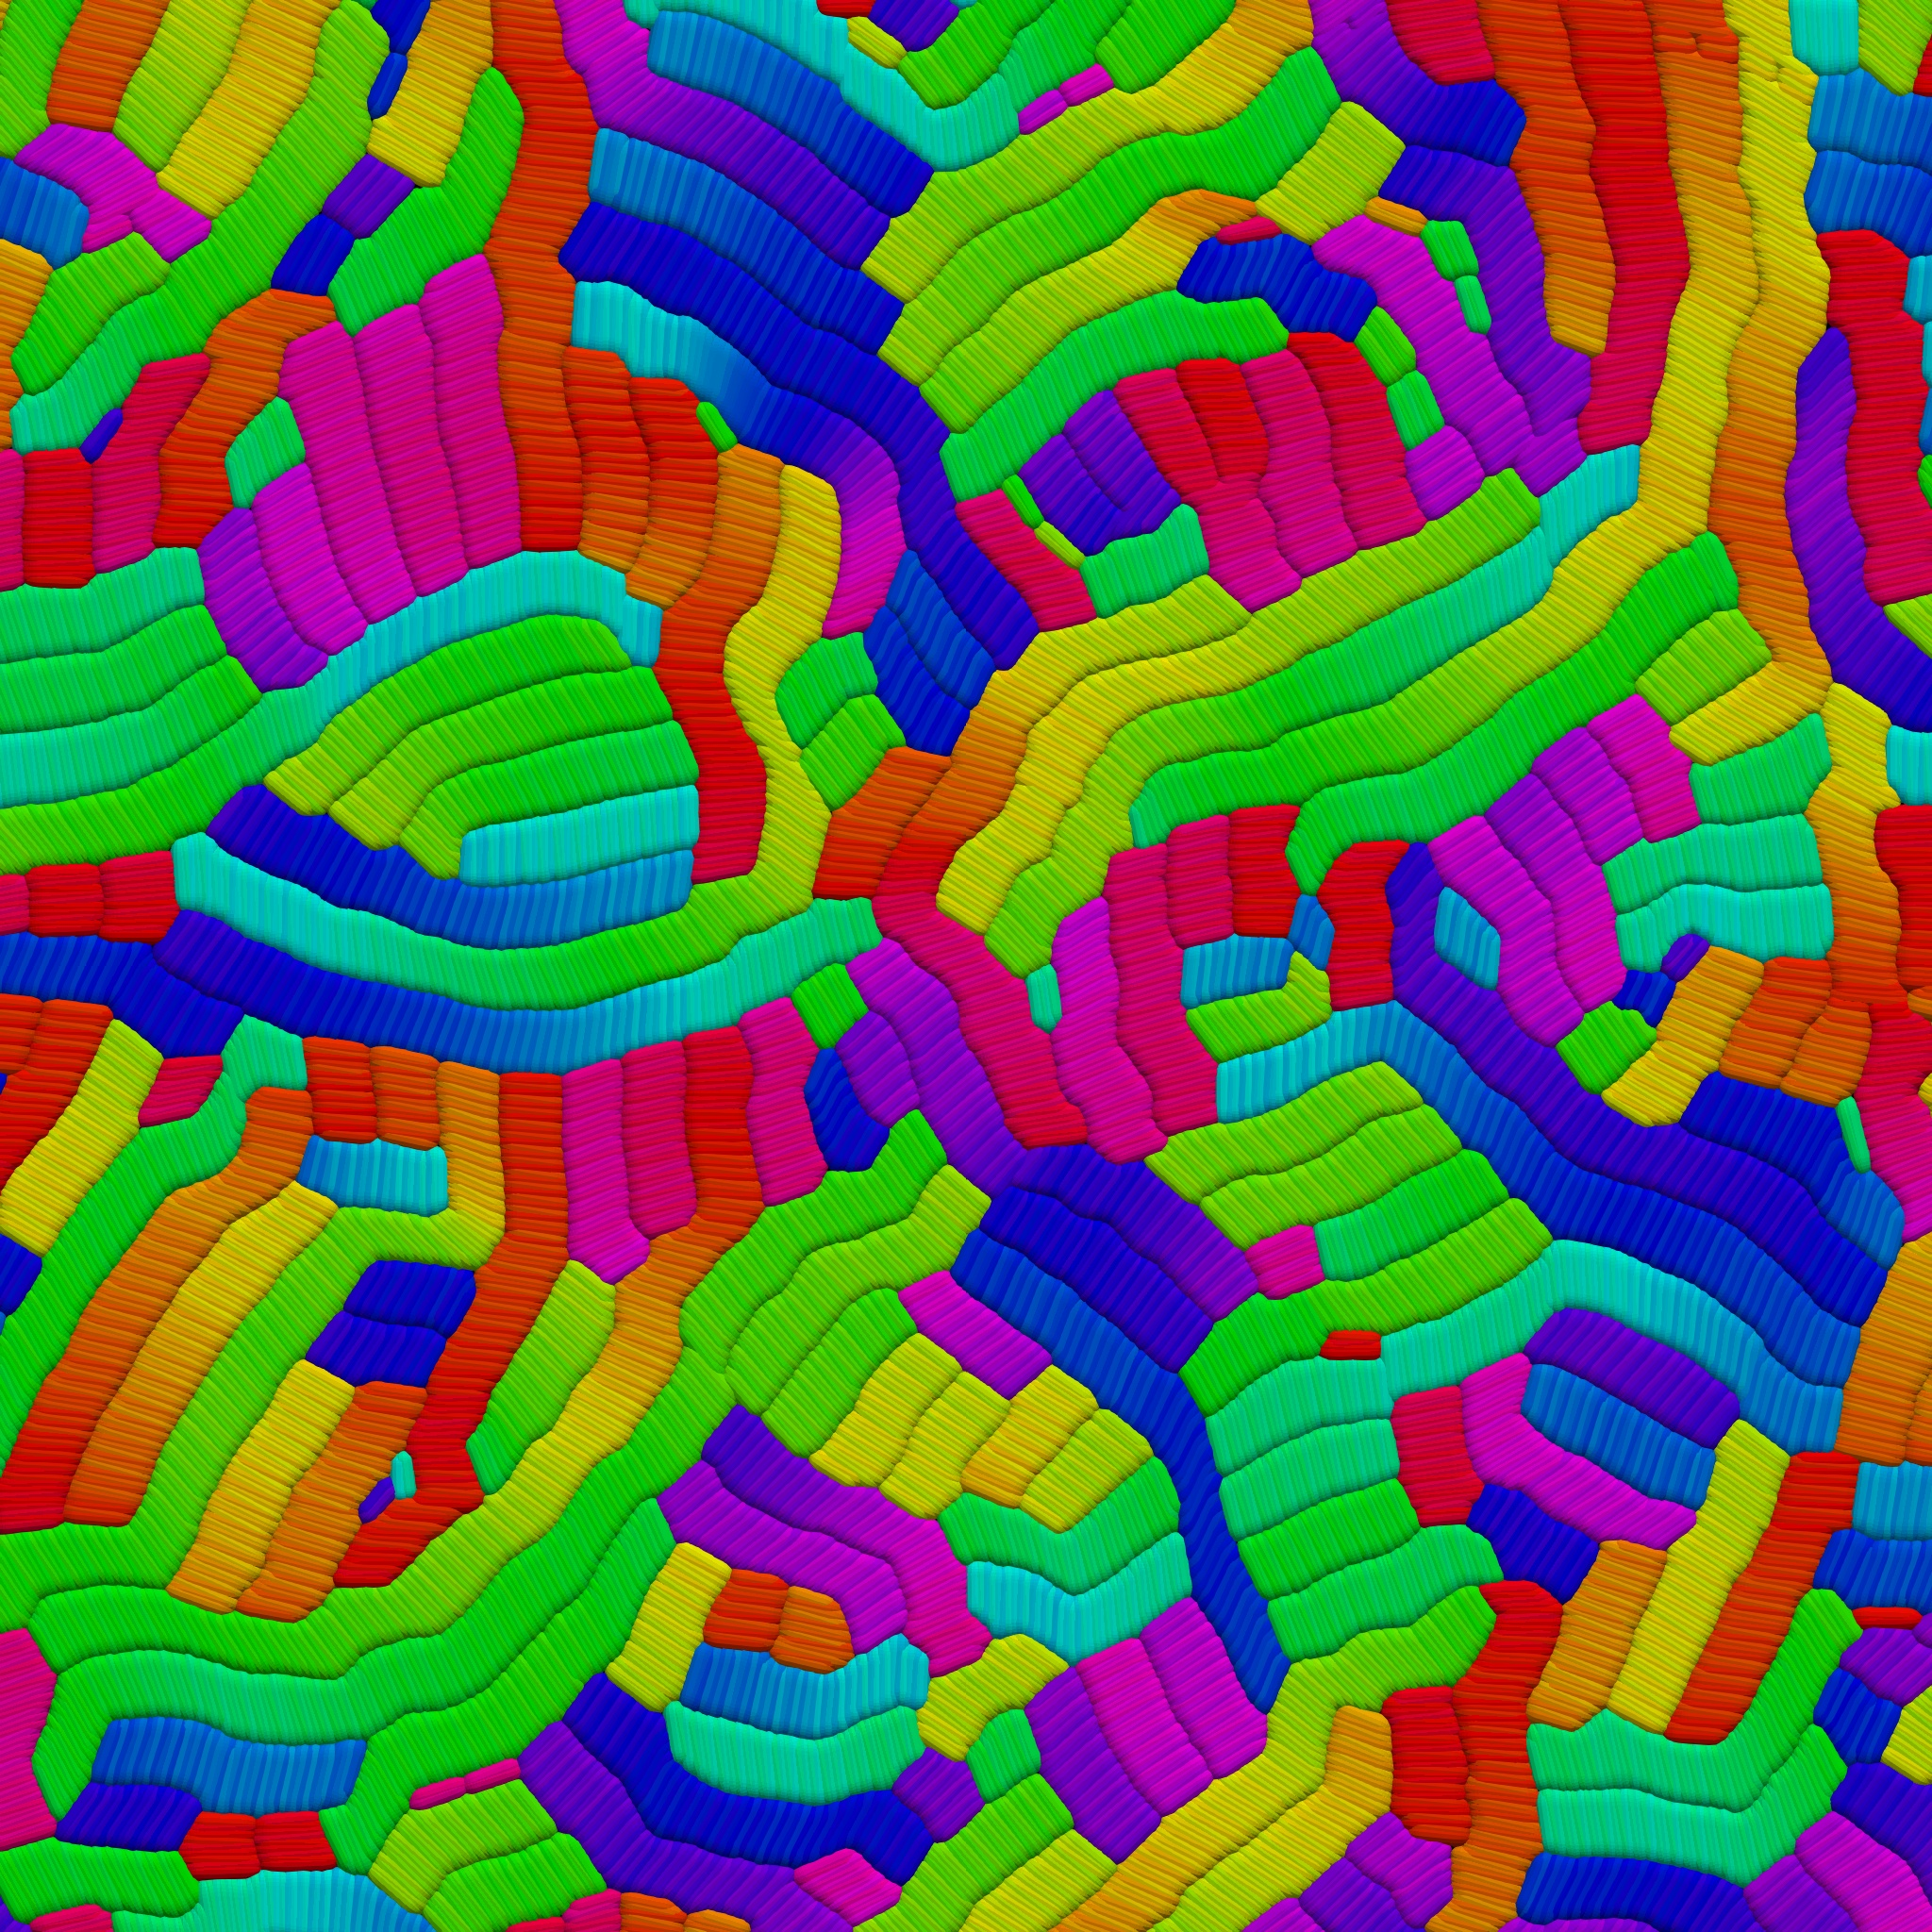
\includegraphics[width=0.62\textwidth]{figures/figures_paper/orientation_comparisons/zoomed_images/soft_e-3_orient.jpeg}
                \caption*{\scriptsize{Soft: elongated bundles}}
            \end{figure}
        \end{column}
    \end{columns}

\end{frame}


% ============================================================
% SECTION 6: COMPUTATIONAL PERFORMANCE
% ============================================================

\section{Computational Performance}

\begin{frame}
    \frametitle{Adaptive Timestepping Strategy}

    \textbf{CFL-based criterion:}
    \begin{equation*}
        \Delta t = \frac{0.5 \, \varepsilon}{u_m}
    \end{equation*}

    where $u_m$ = median cell velocity, $\varepsilon = 10^{-3}$ = tolerance

    \vspace{0.5cm}

    \textbf{Benefits:}
    \begin{itemize}
        \item Prevents excessive motion per step
        \item Adapts to colony dynamics
        \item Maintains numerical stability
        \item Essential for both models
    \end{itemize}

\end{frame}

\begin{frame}
    \frametitle{The Timestep Divide}

    \begin{figure}
        \centering
        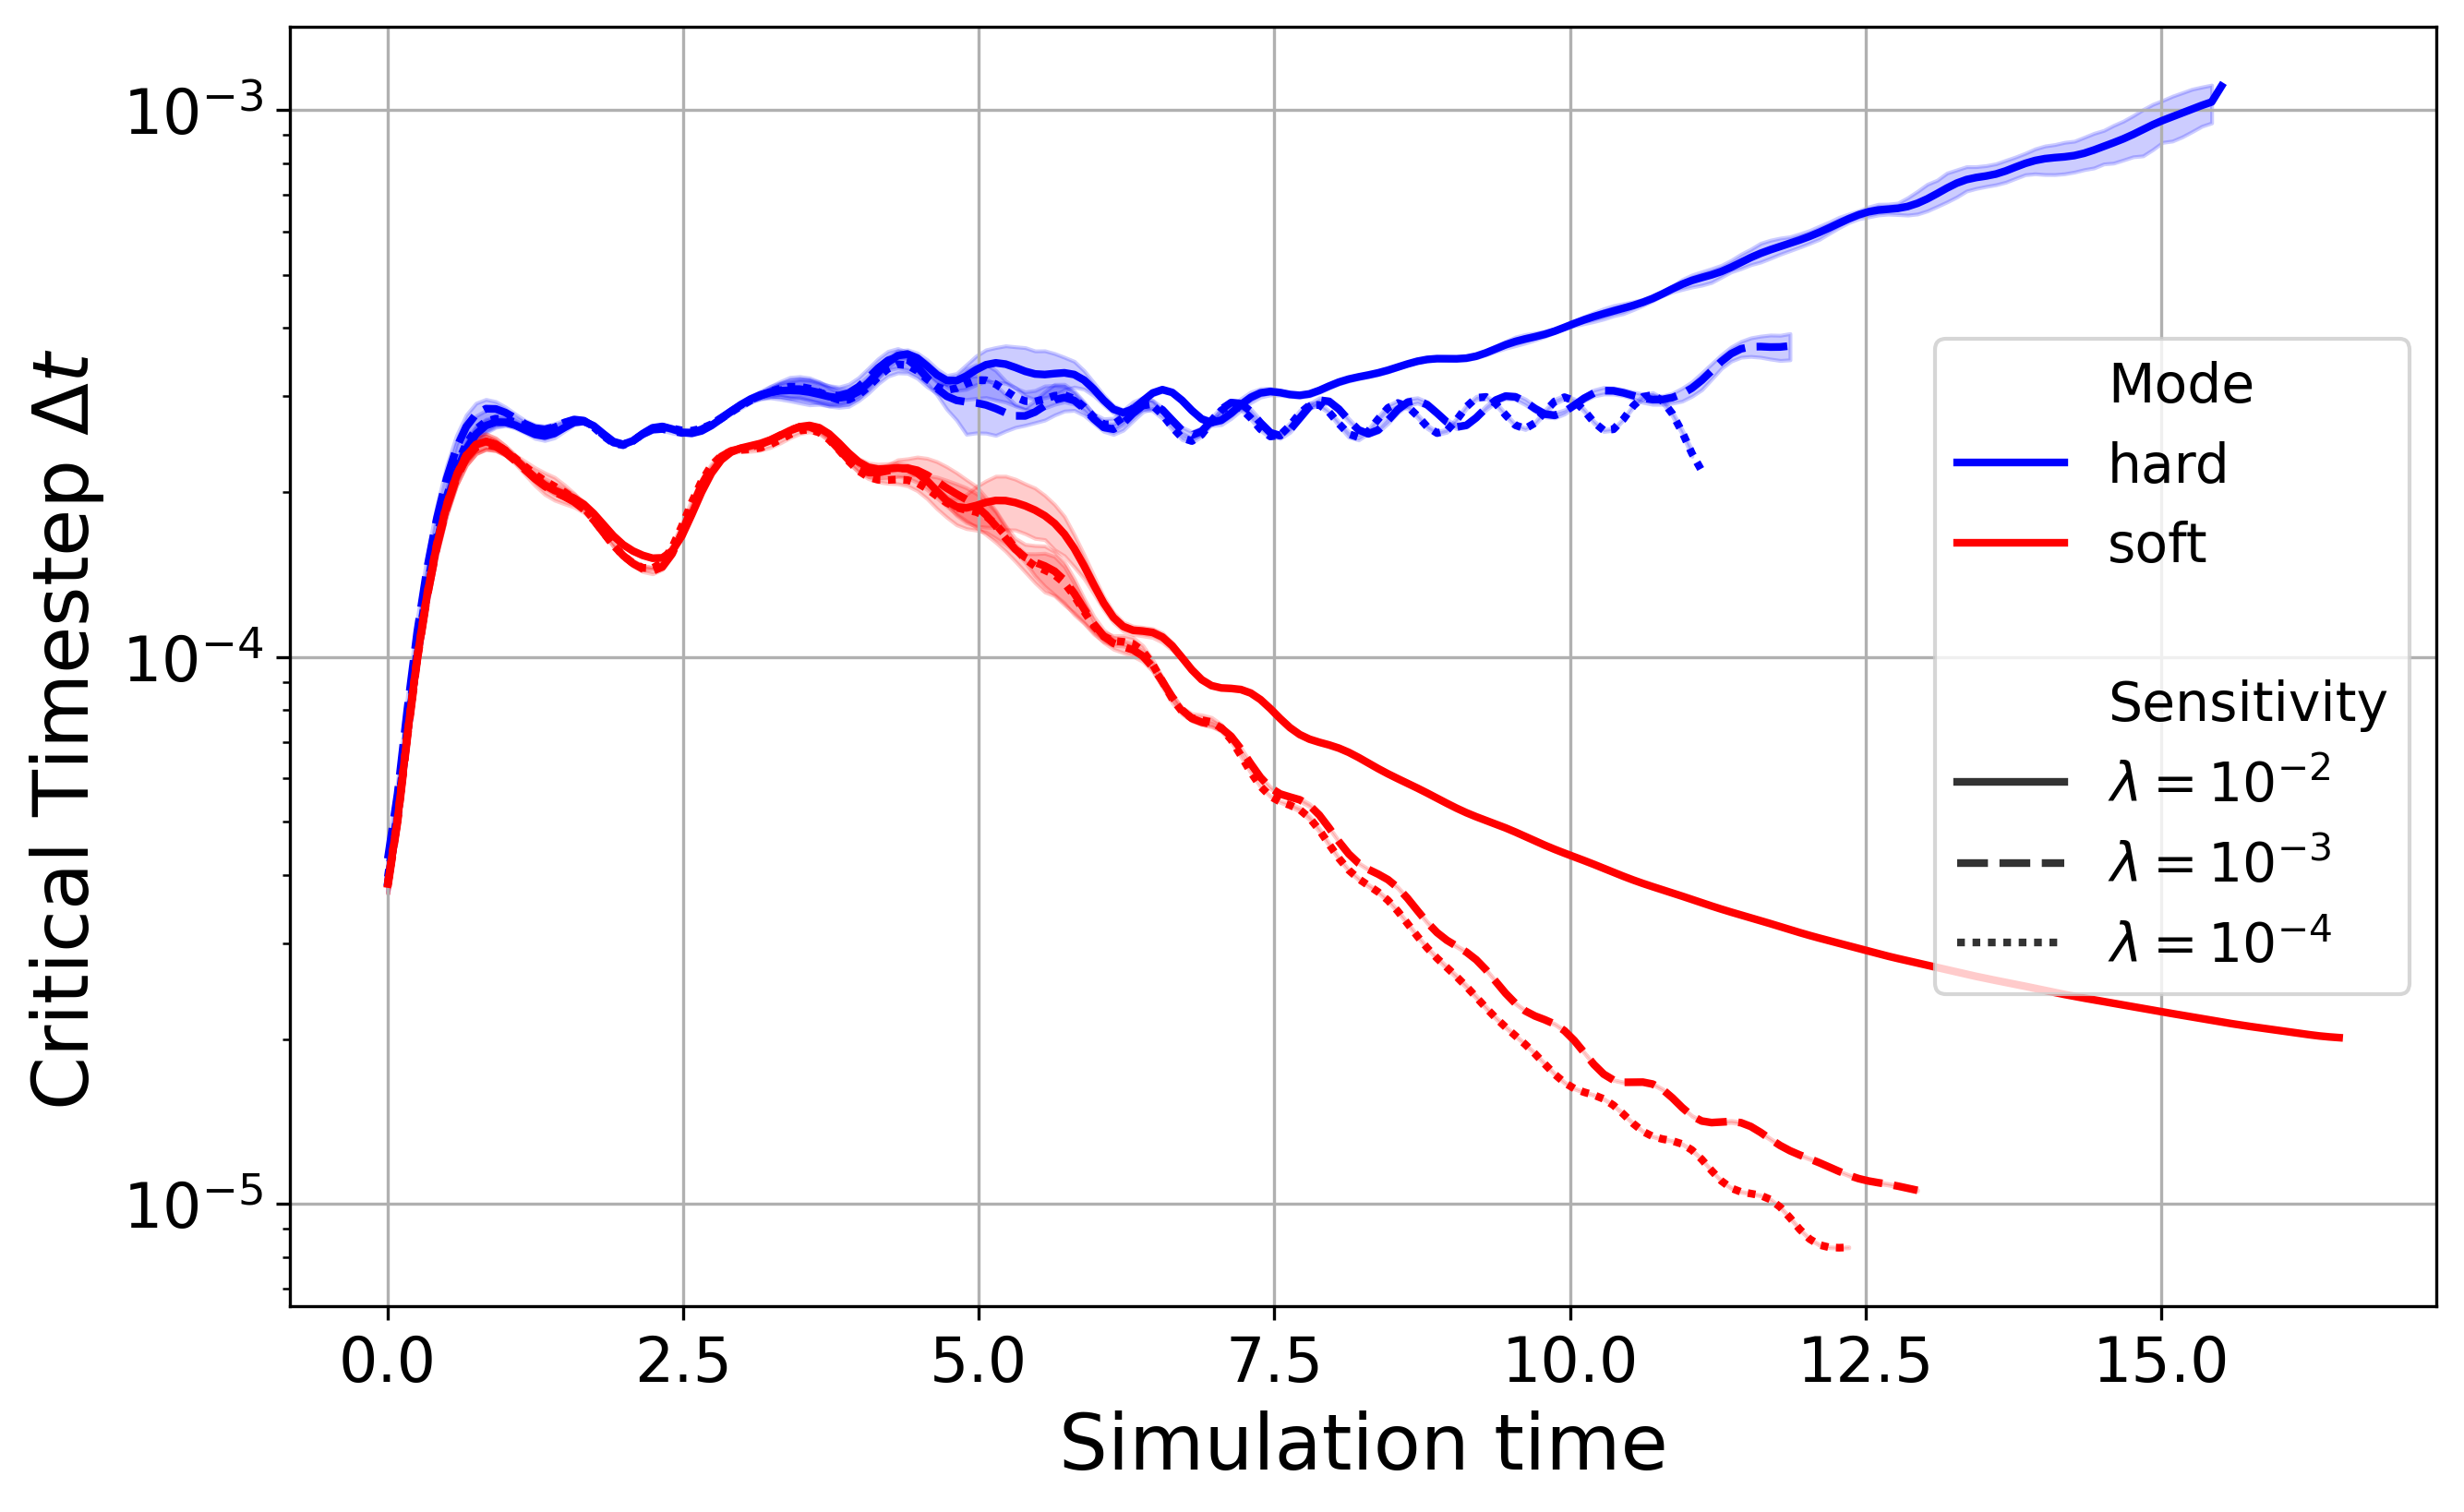
\includegraphics[width=0.8\textwidth]{figures/figures_paper/comparison_plots/combined_simulation_time_vs_dt.png}
    \end{figure}

\end{frame}


\begin{frame}
    \frametitle{Parallel Architecture}

    \begin{columns}
        \begin{column}{0.5\textwidth}
            \textbf{Implementation:}
            \begin{itemize}
                \item MPI + PETSc framework
                \item Distributed vectors/matrices
                \item Angular sector decomposition
                \item Ghost particle exchange
            \end{itemize}

            \vspace{0.3cm}

            \textbf{Benchmarking:}
            \begin{itemize}
                \item CoolMUC-4 cluster
                \item Up to 112 cores
            \end{itemize}
        \end{column}

        \begin{column}{0.5\textwidth}
            \vspace{-1cm}
            \begin{figure}
                \centering
                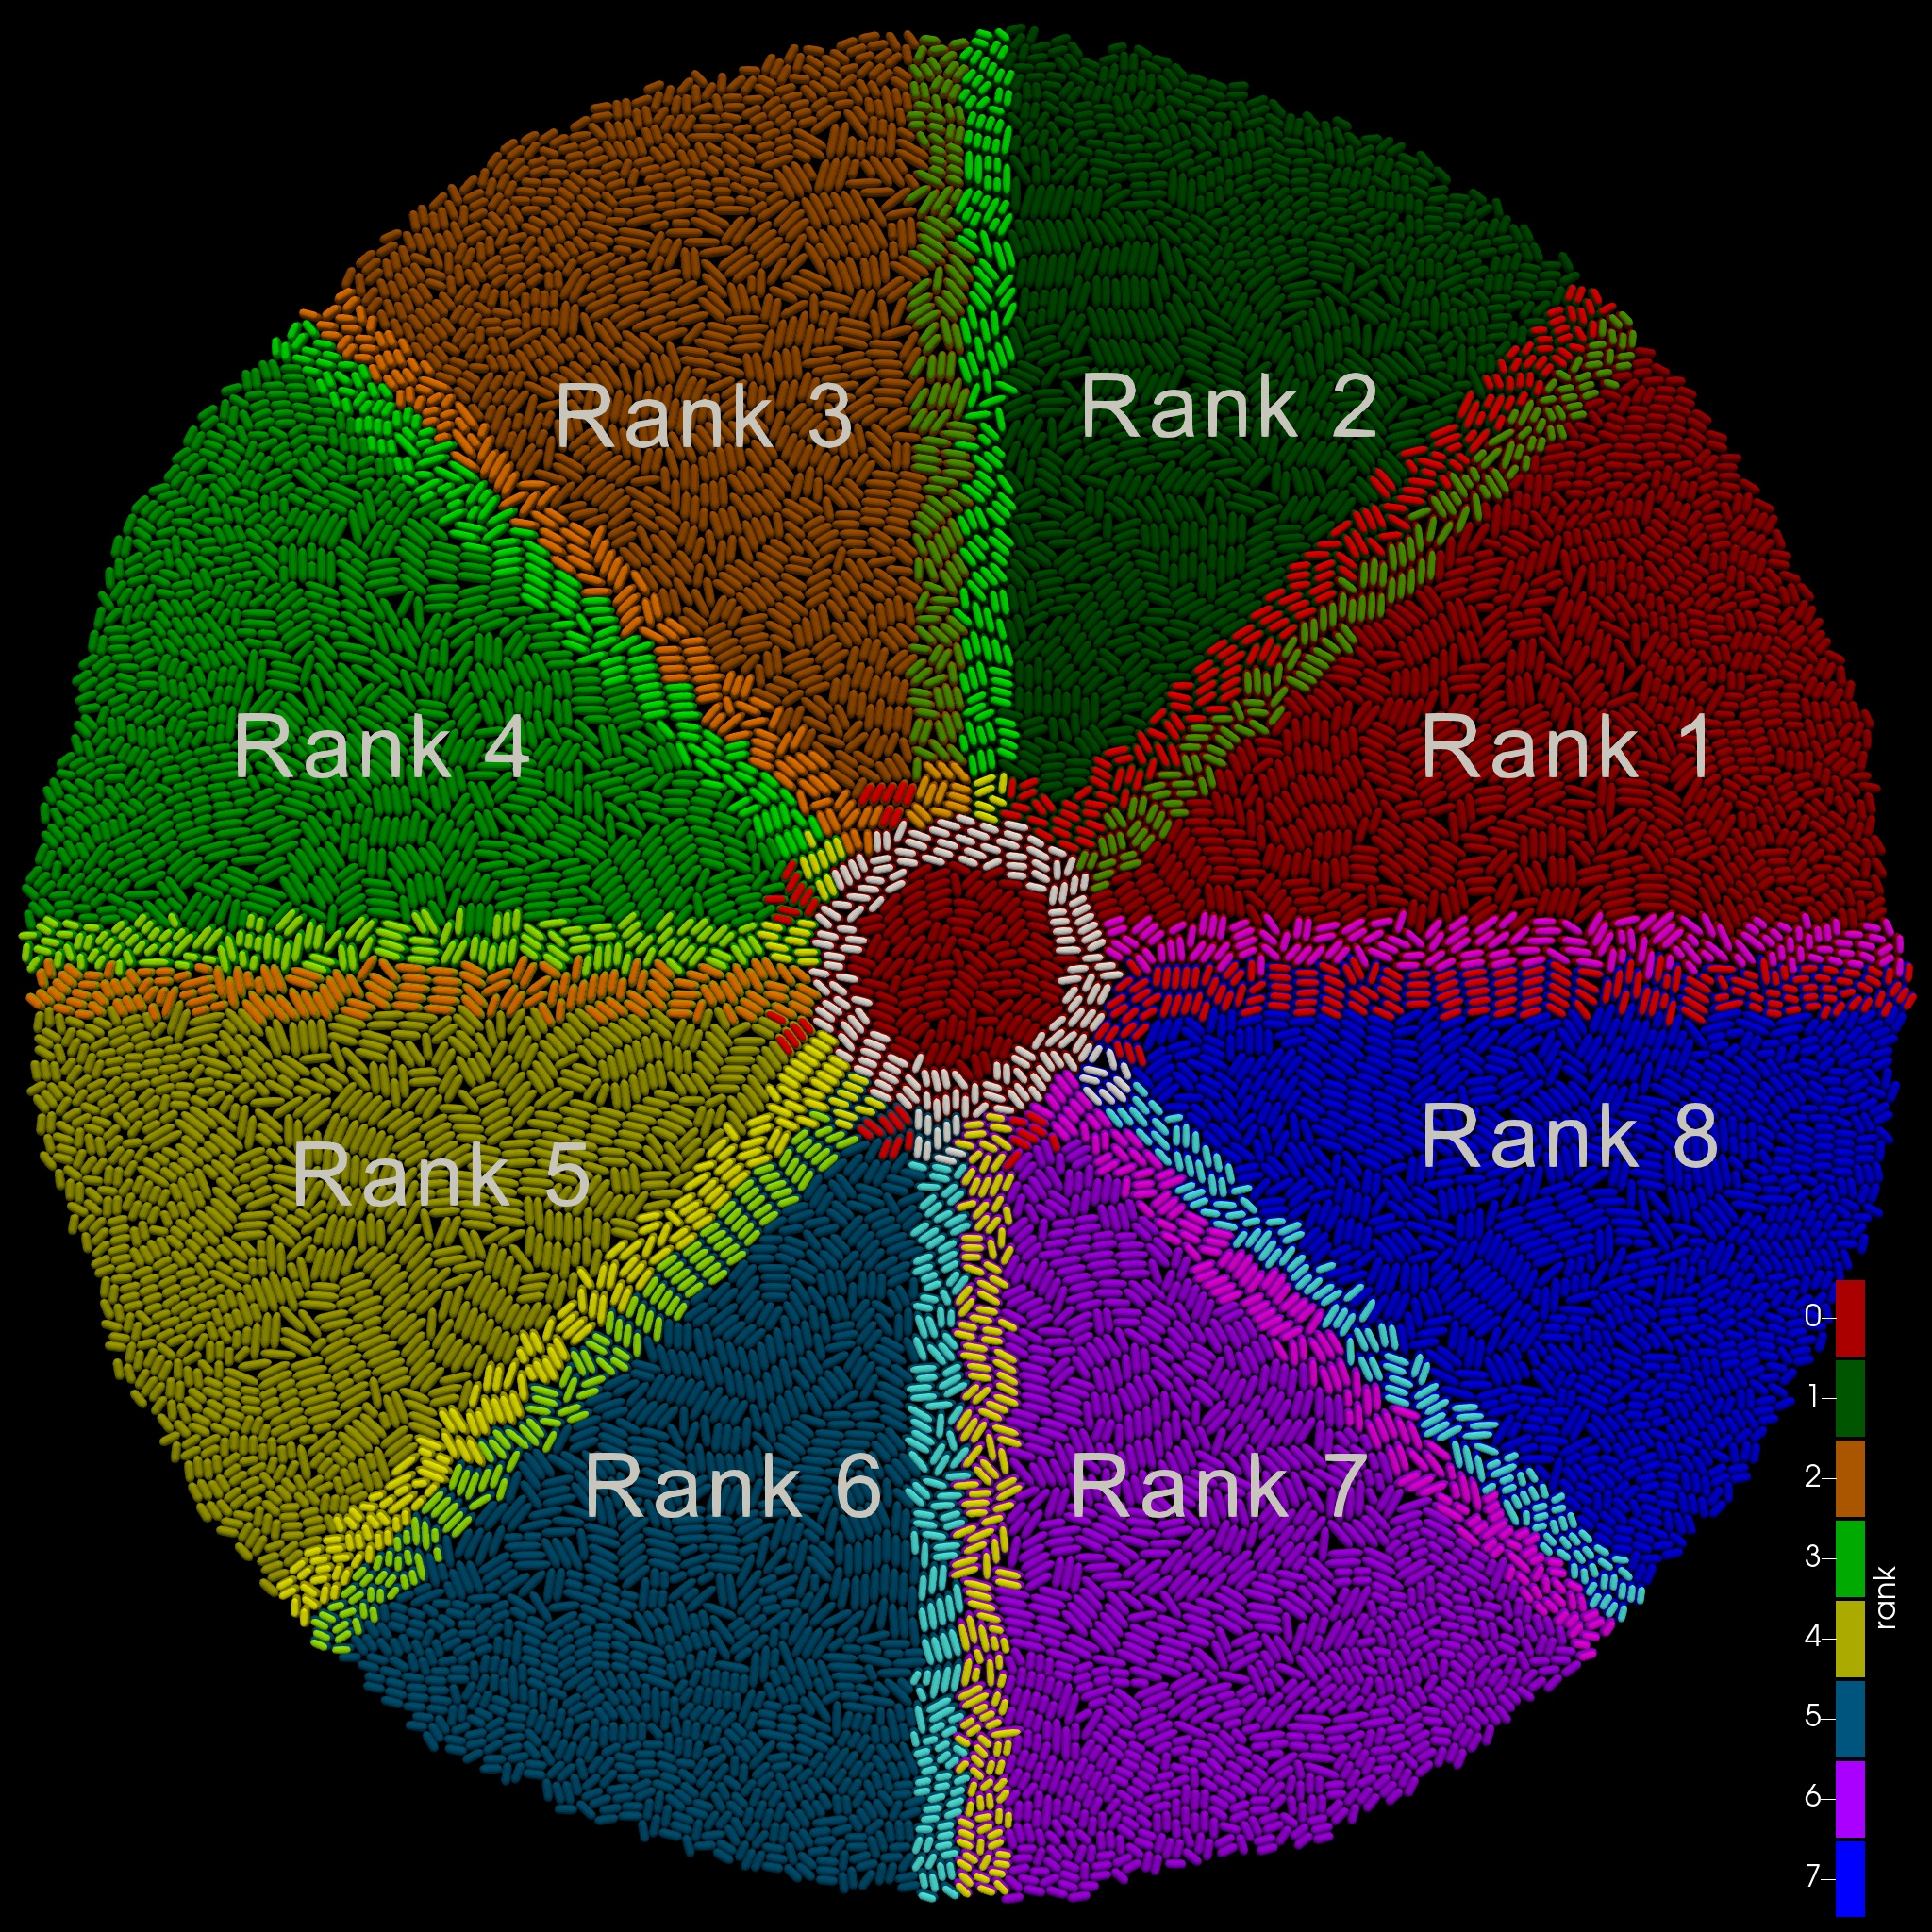
\includegraphics[width=\textwidth]{figures/figures_paper/runtimes/domain_decomposition.jpeg}
                \caption*{\scriptsize{Domain decomposition with 8 MPI ranks}}
            \end{figure}
        \end{column}
    \end{columns}

\end{frame}

\begin{frame}
    \frametitle{Strong Scaling: Runtime to reach $R=100$}

    \begin{figure}
        \centering
        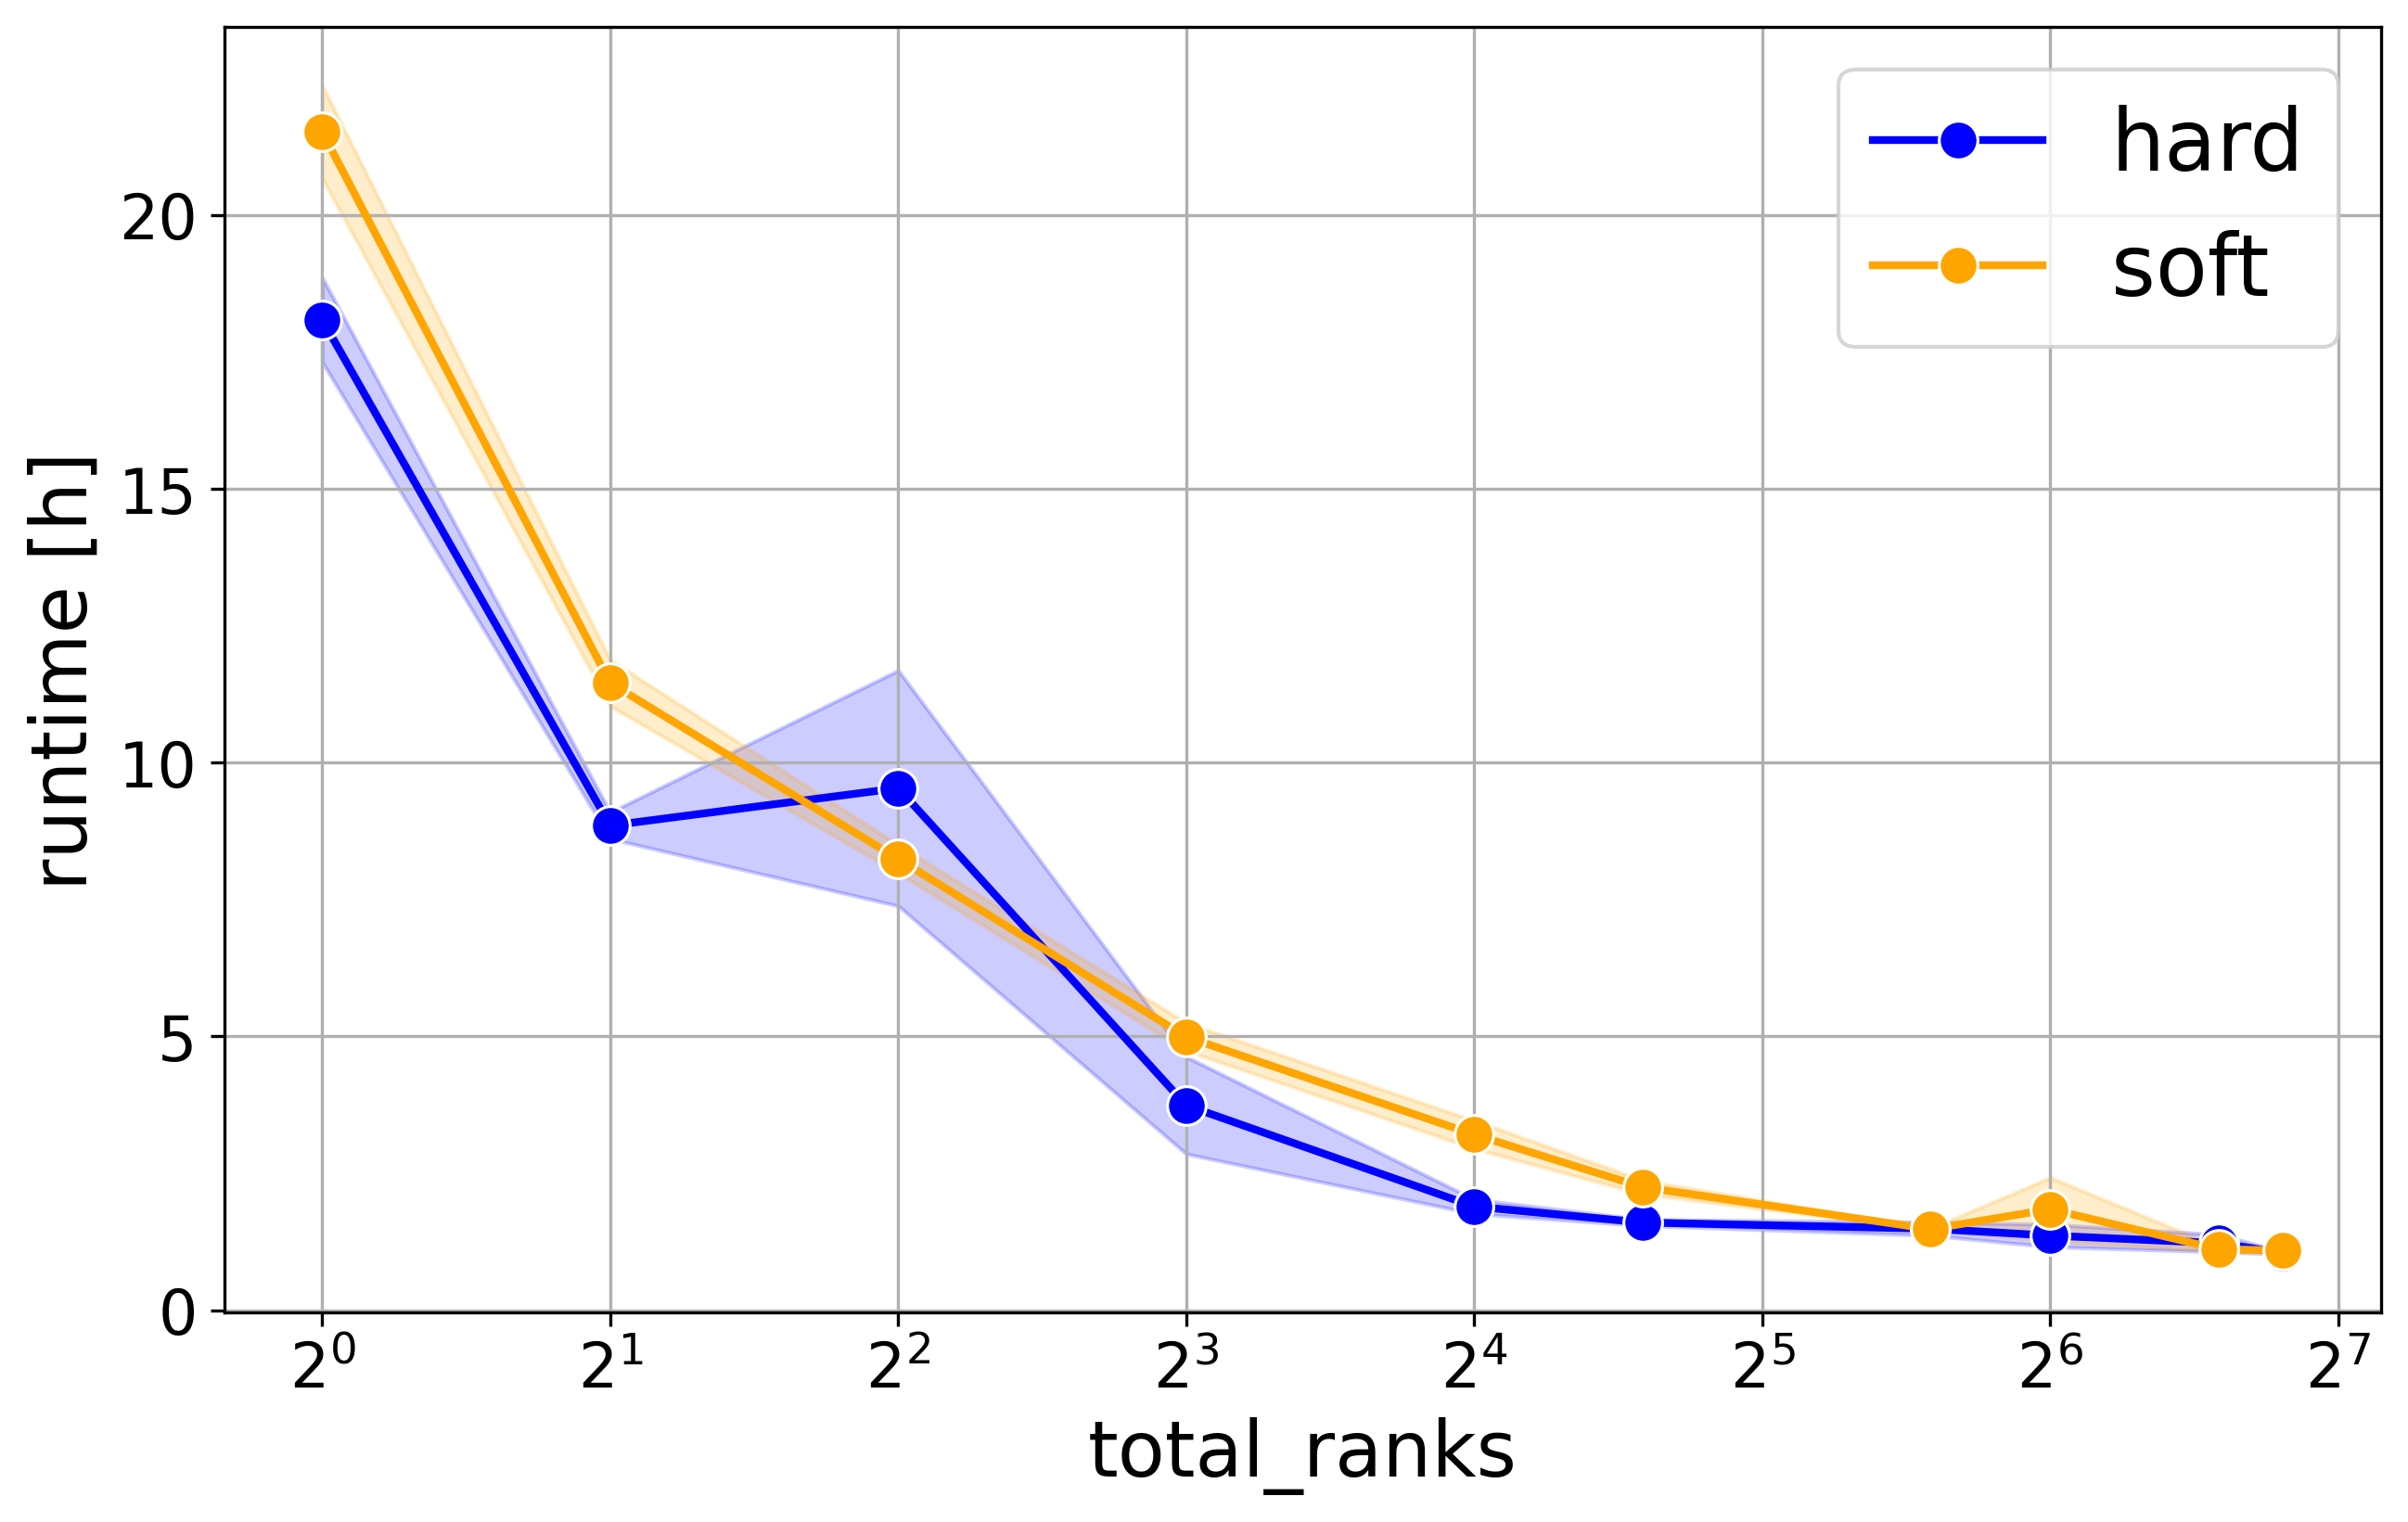
\includegraphics[width=0.8\textwidth]{figures/figures_paper/runtimes/strong_scaling_runtime_hard_soft.png}
    \end{figure}

    \textbf{Key results:}
    \begin{itemize}
        \item Hard model is always faster!
        \item Both model slow down at high core counts
    \end{itemize}

\end{frame}

\begin{frame}
    \frametitle{Strong Scaling: Speedup}

    \begin{figure}
        \centering
        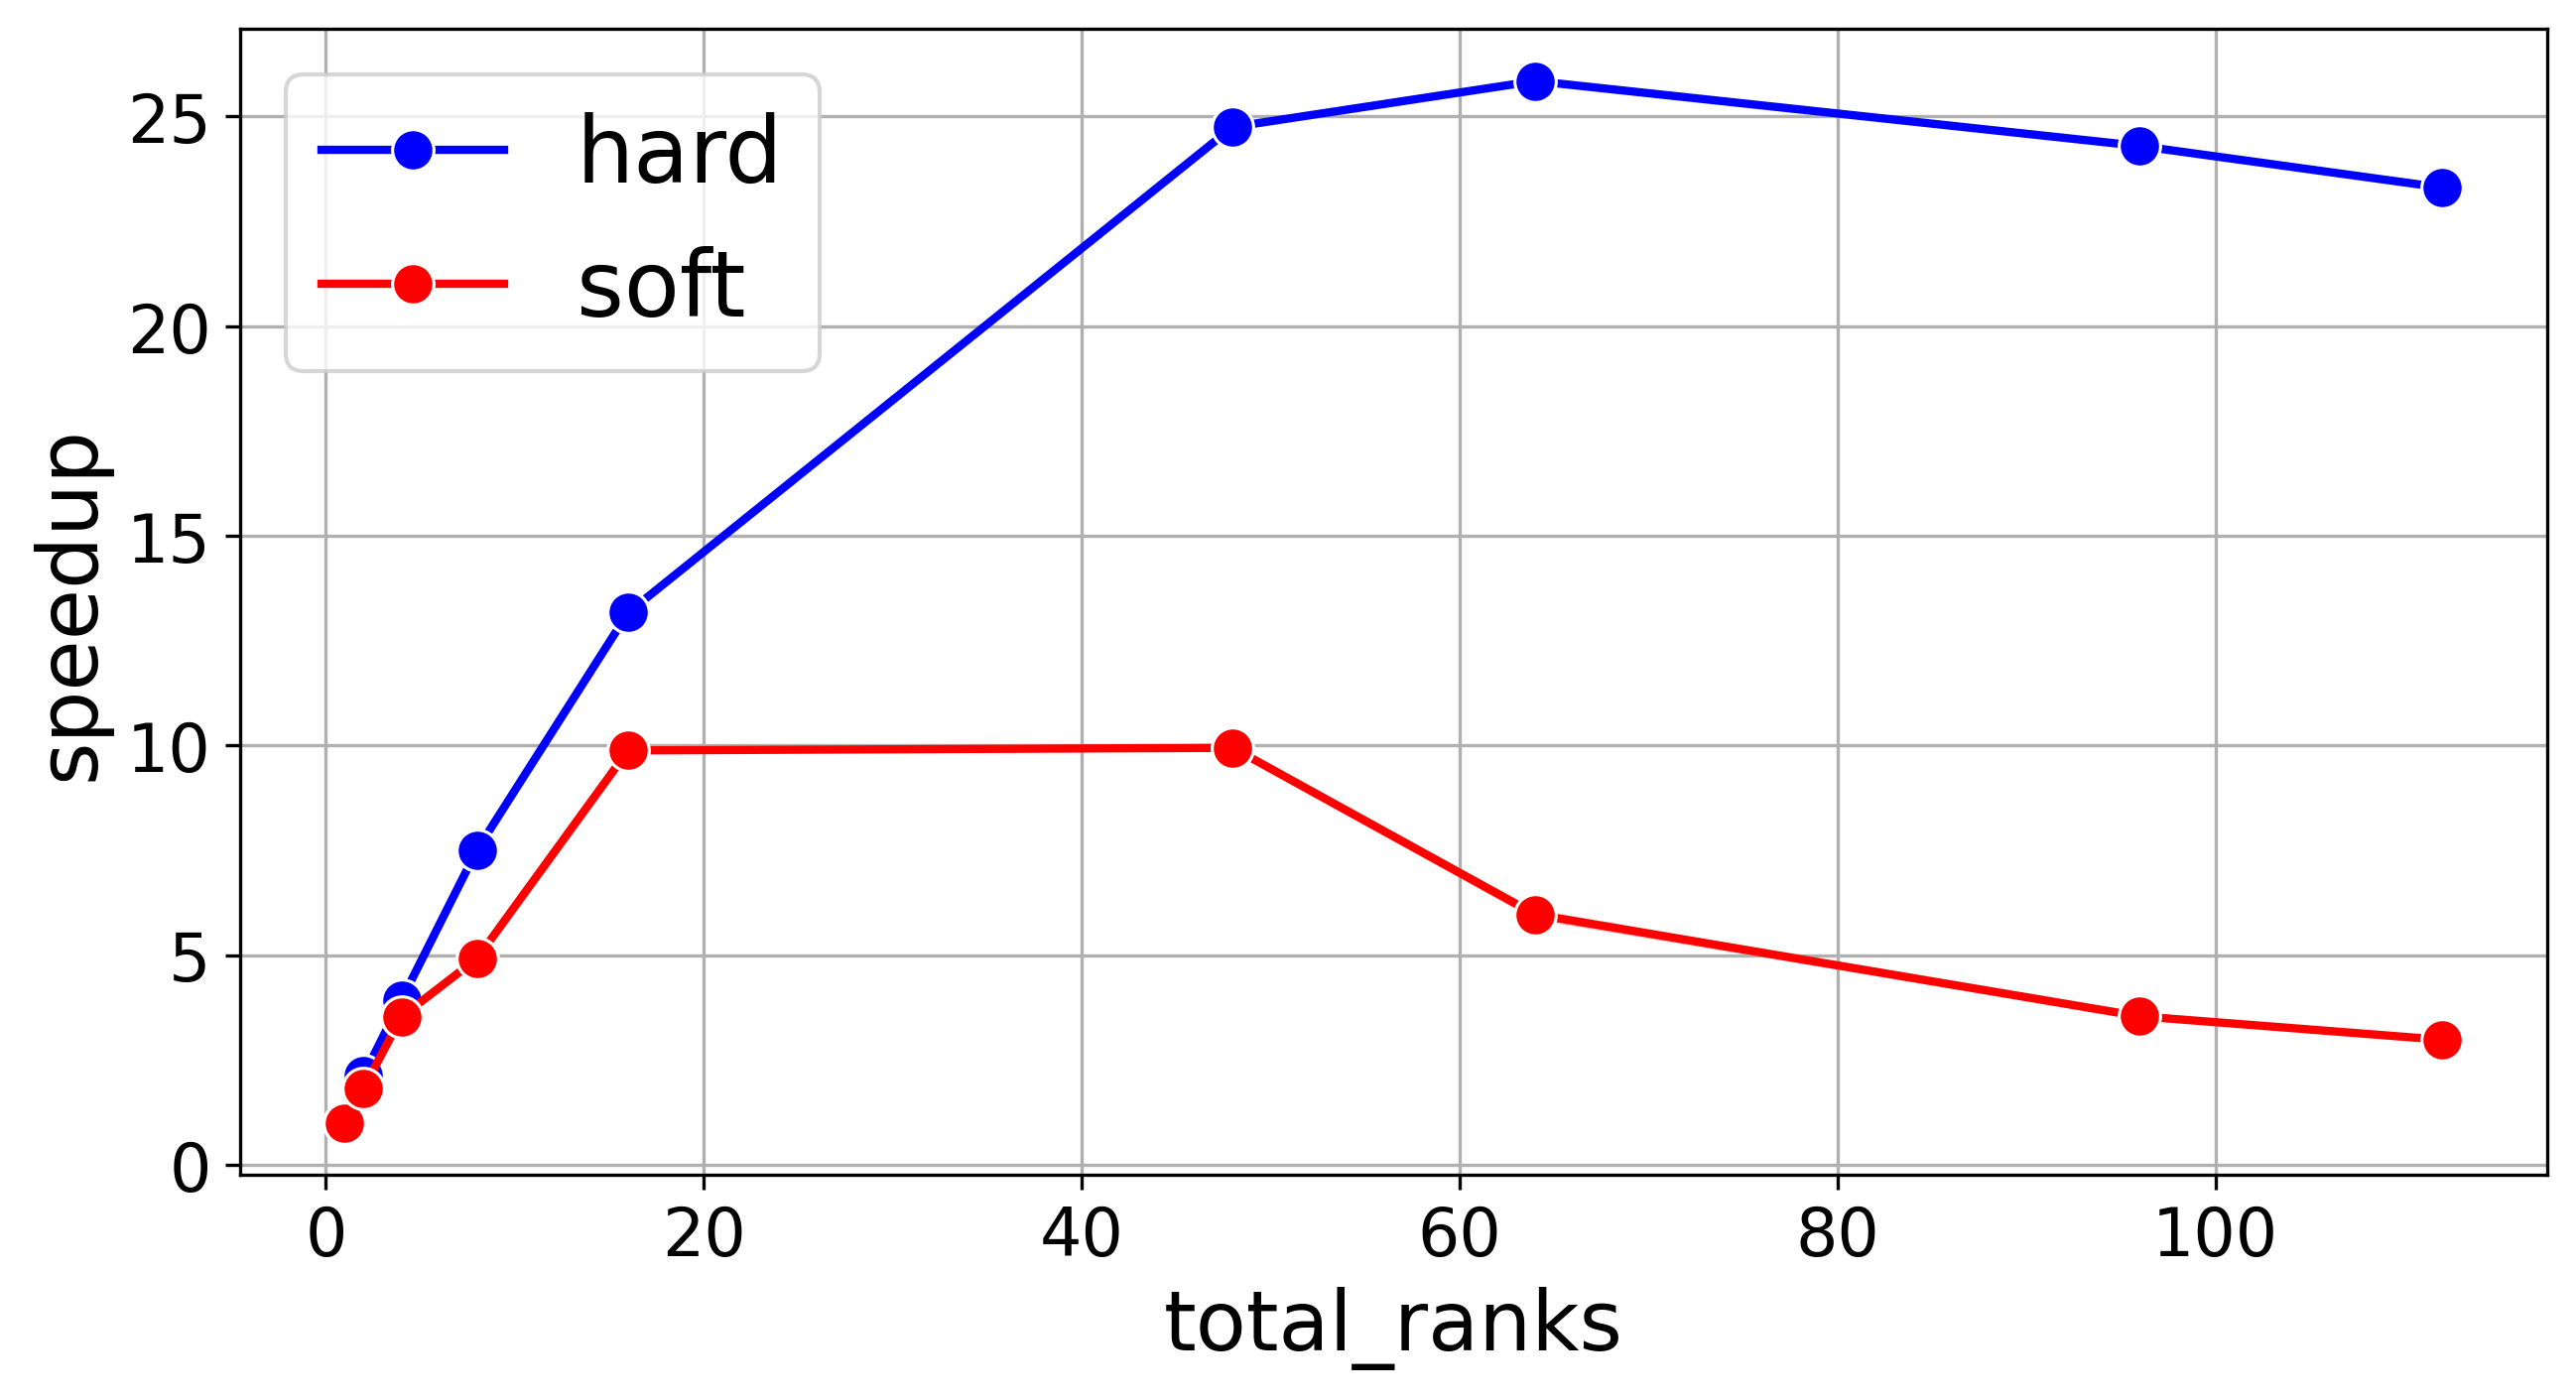
\includegraphics[width=0.8\textwidth]{figures/figures_paper/runtimes/strong_scaling_speedup_hard_soft.png}
    \end{figure}

    \textbf{Scaling limits:}
    \begin{itemize}
        \item Communication overhead dominates at high ranks
        \item Larger timesteps amortize communication costs
    \end{itemize}

\end{frame}

\begin{frame}
    \frametitle{Maximum Colony Size (24h budget, 112 cores)}

    \begin{columns}
        \begin{column}{0.4\textwidth}
            \textbf{Hard Model:}
            \begin{itemize}
                \item $R_{\max} = 260$
                \item 301,116 cells
                \item Maintains accuracy
                \item Larger accessible scales
            \end{itemize}

            \vspace{0.5cm}

            \textbf{Scaling:}
            \begin{itemize}
                \item $T[h] \propto R^5 \propto N^{2.5}$
                \item $\mathcal{O}(N)$ BBPGD iterations per step
                \item Many sparse matrix-vector products
            \end{itemize}
        \end{column}

        \begin{column}{0.6\textwidth}
            \begin{figure}
                \centering
                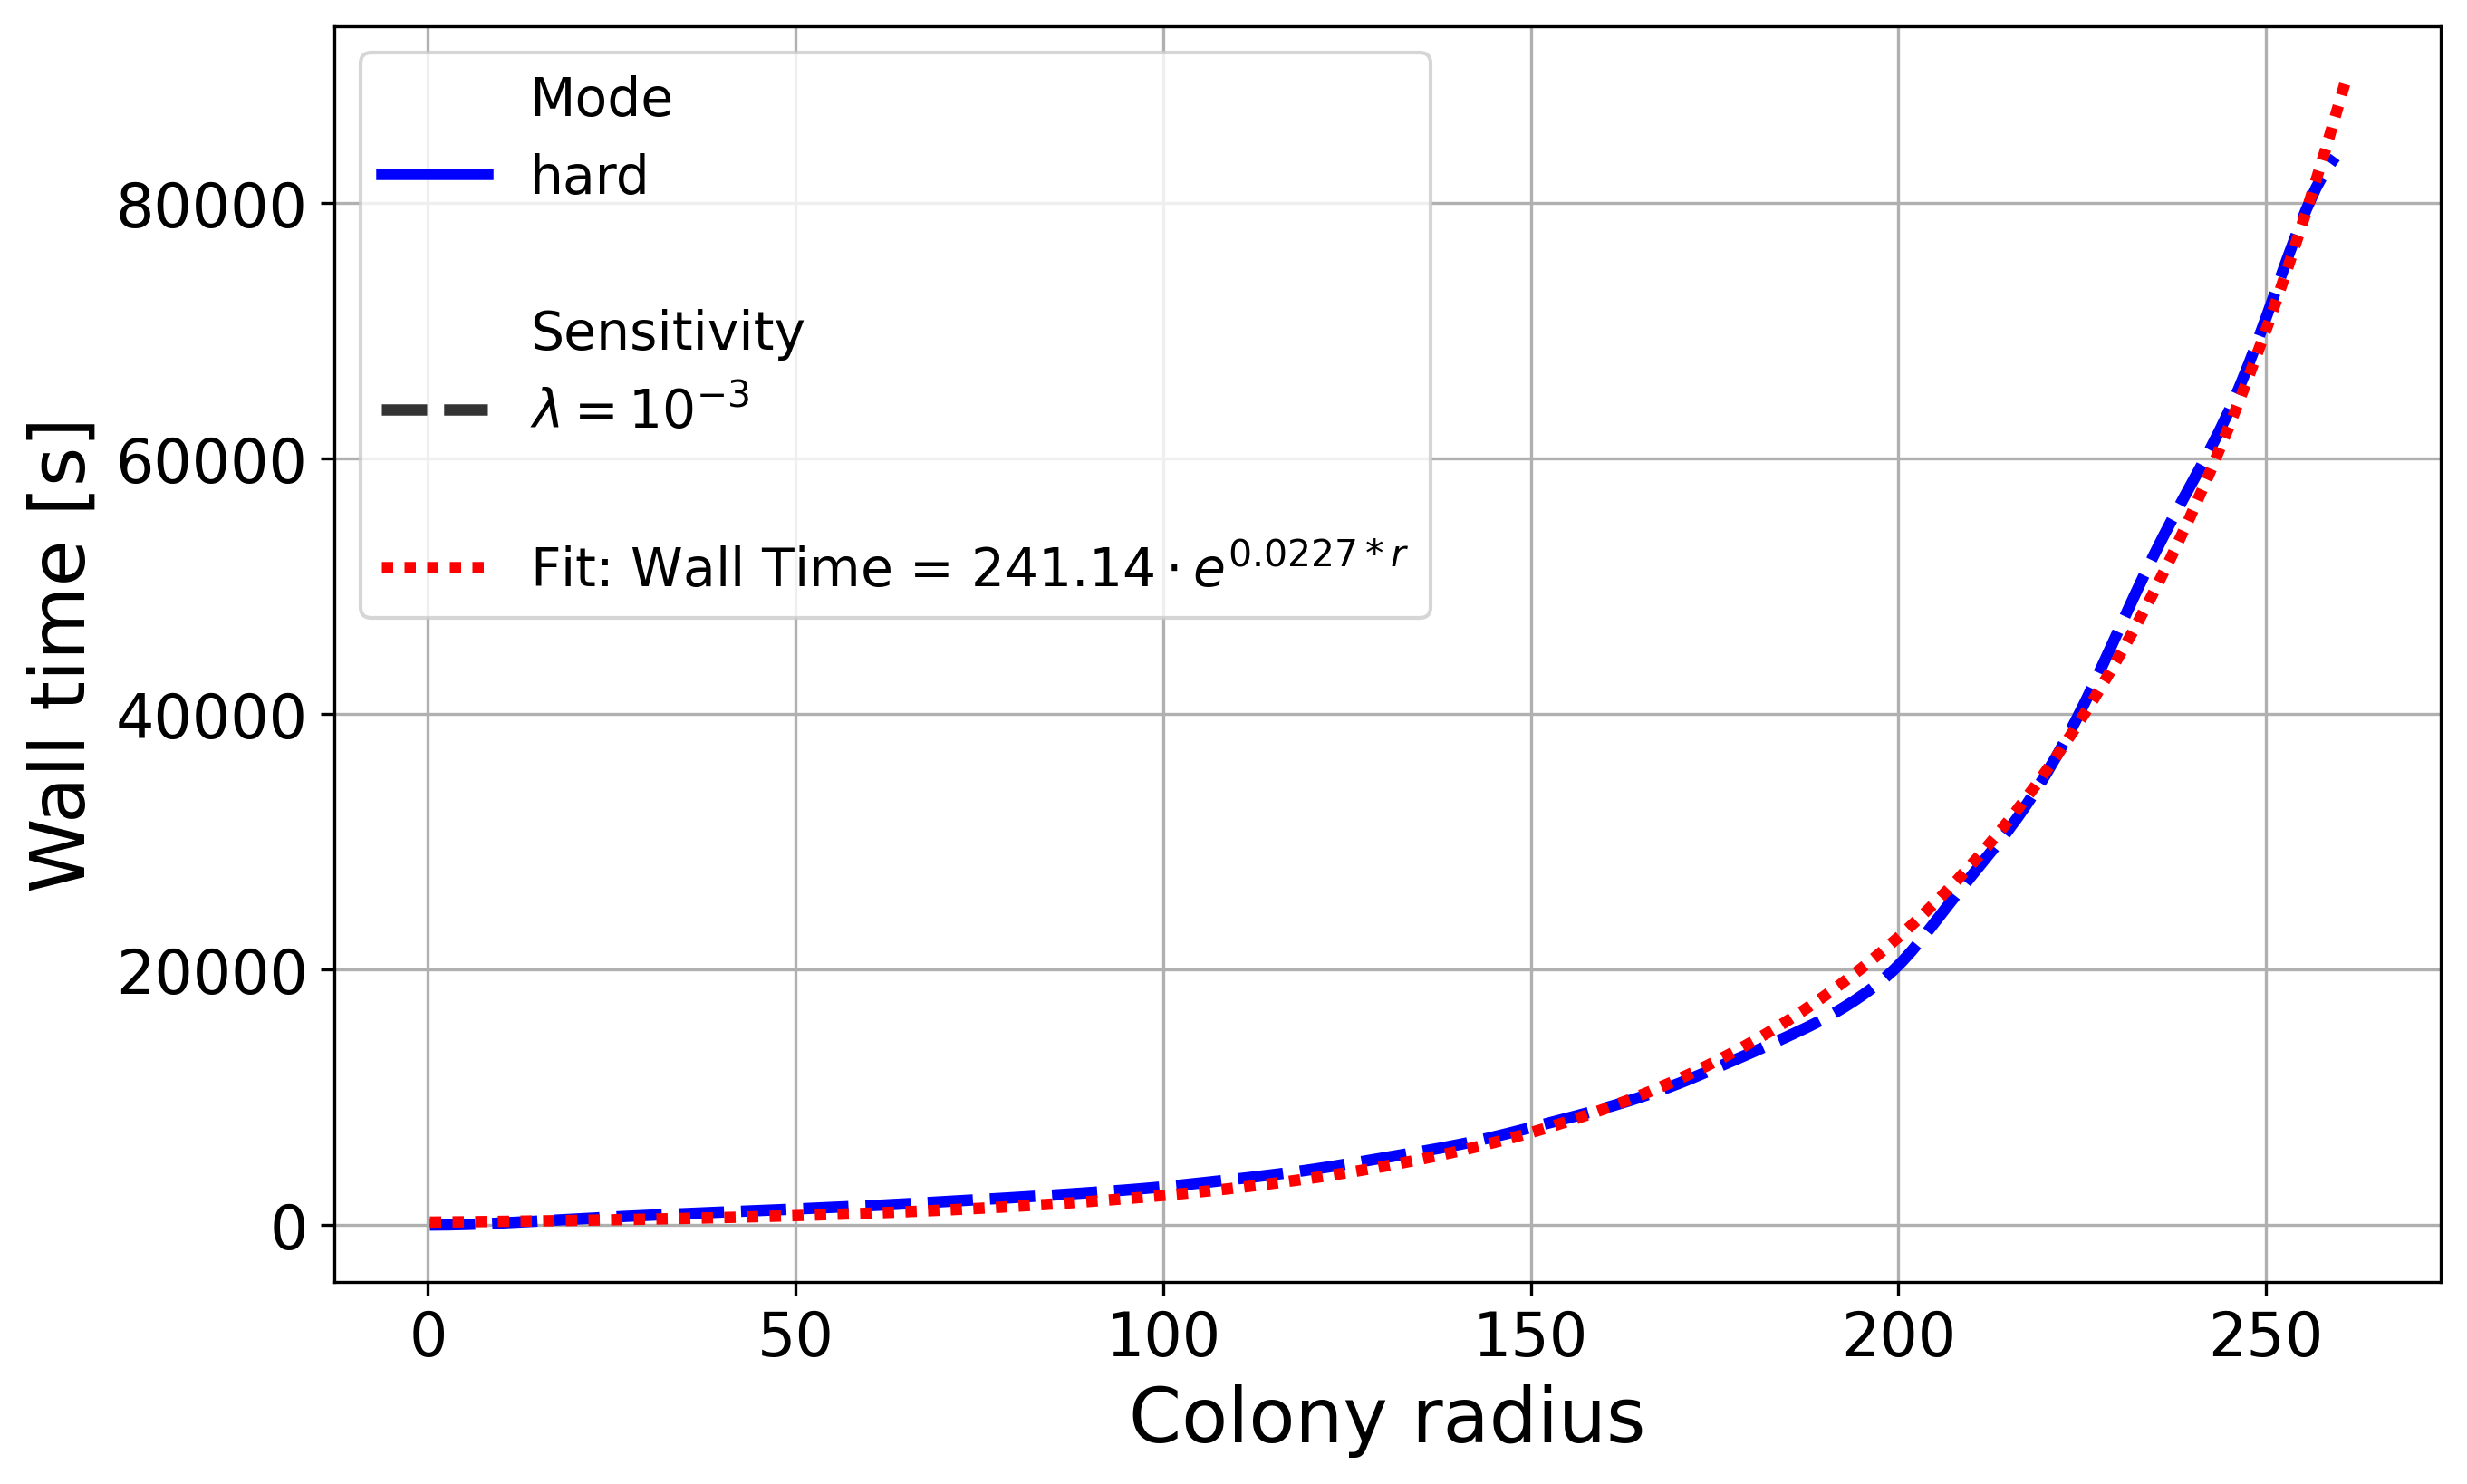
\includegraphics[width=\textwidth]{figures/figures_paper/huge/huge_wall_time_vs_radius_with_fit.png}
            \end{figure}
        \end{column}

    \end{columns}

\end{frame}

\begin{frame}
    \frametitle{BBPGD Solver Performance}

    \begin{figure}
        \centering
        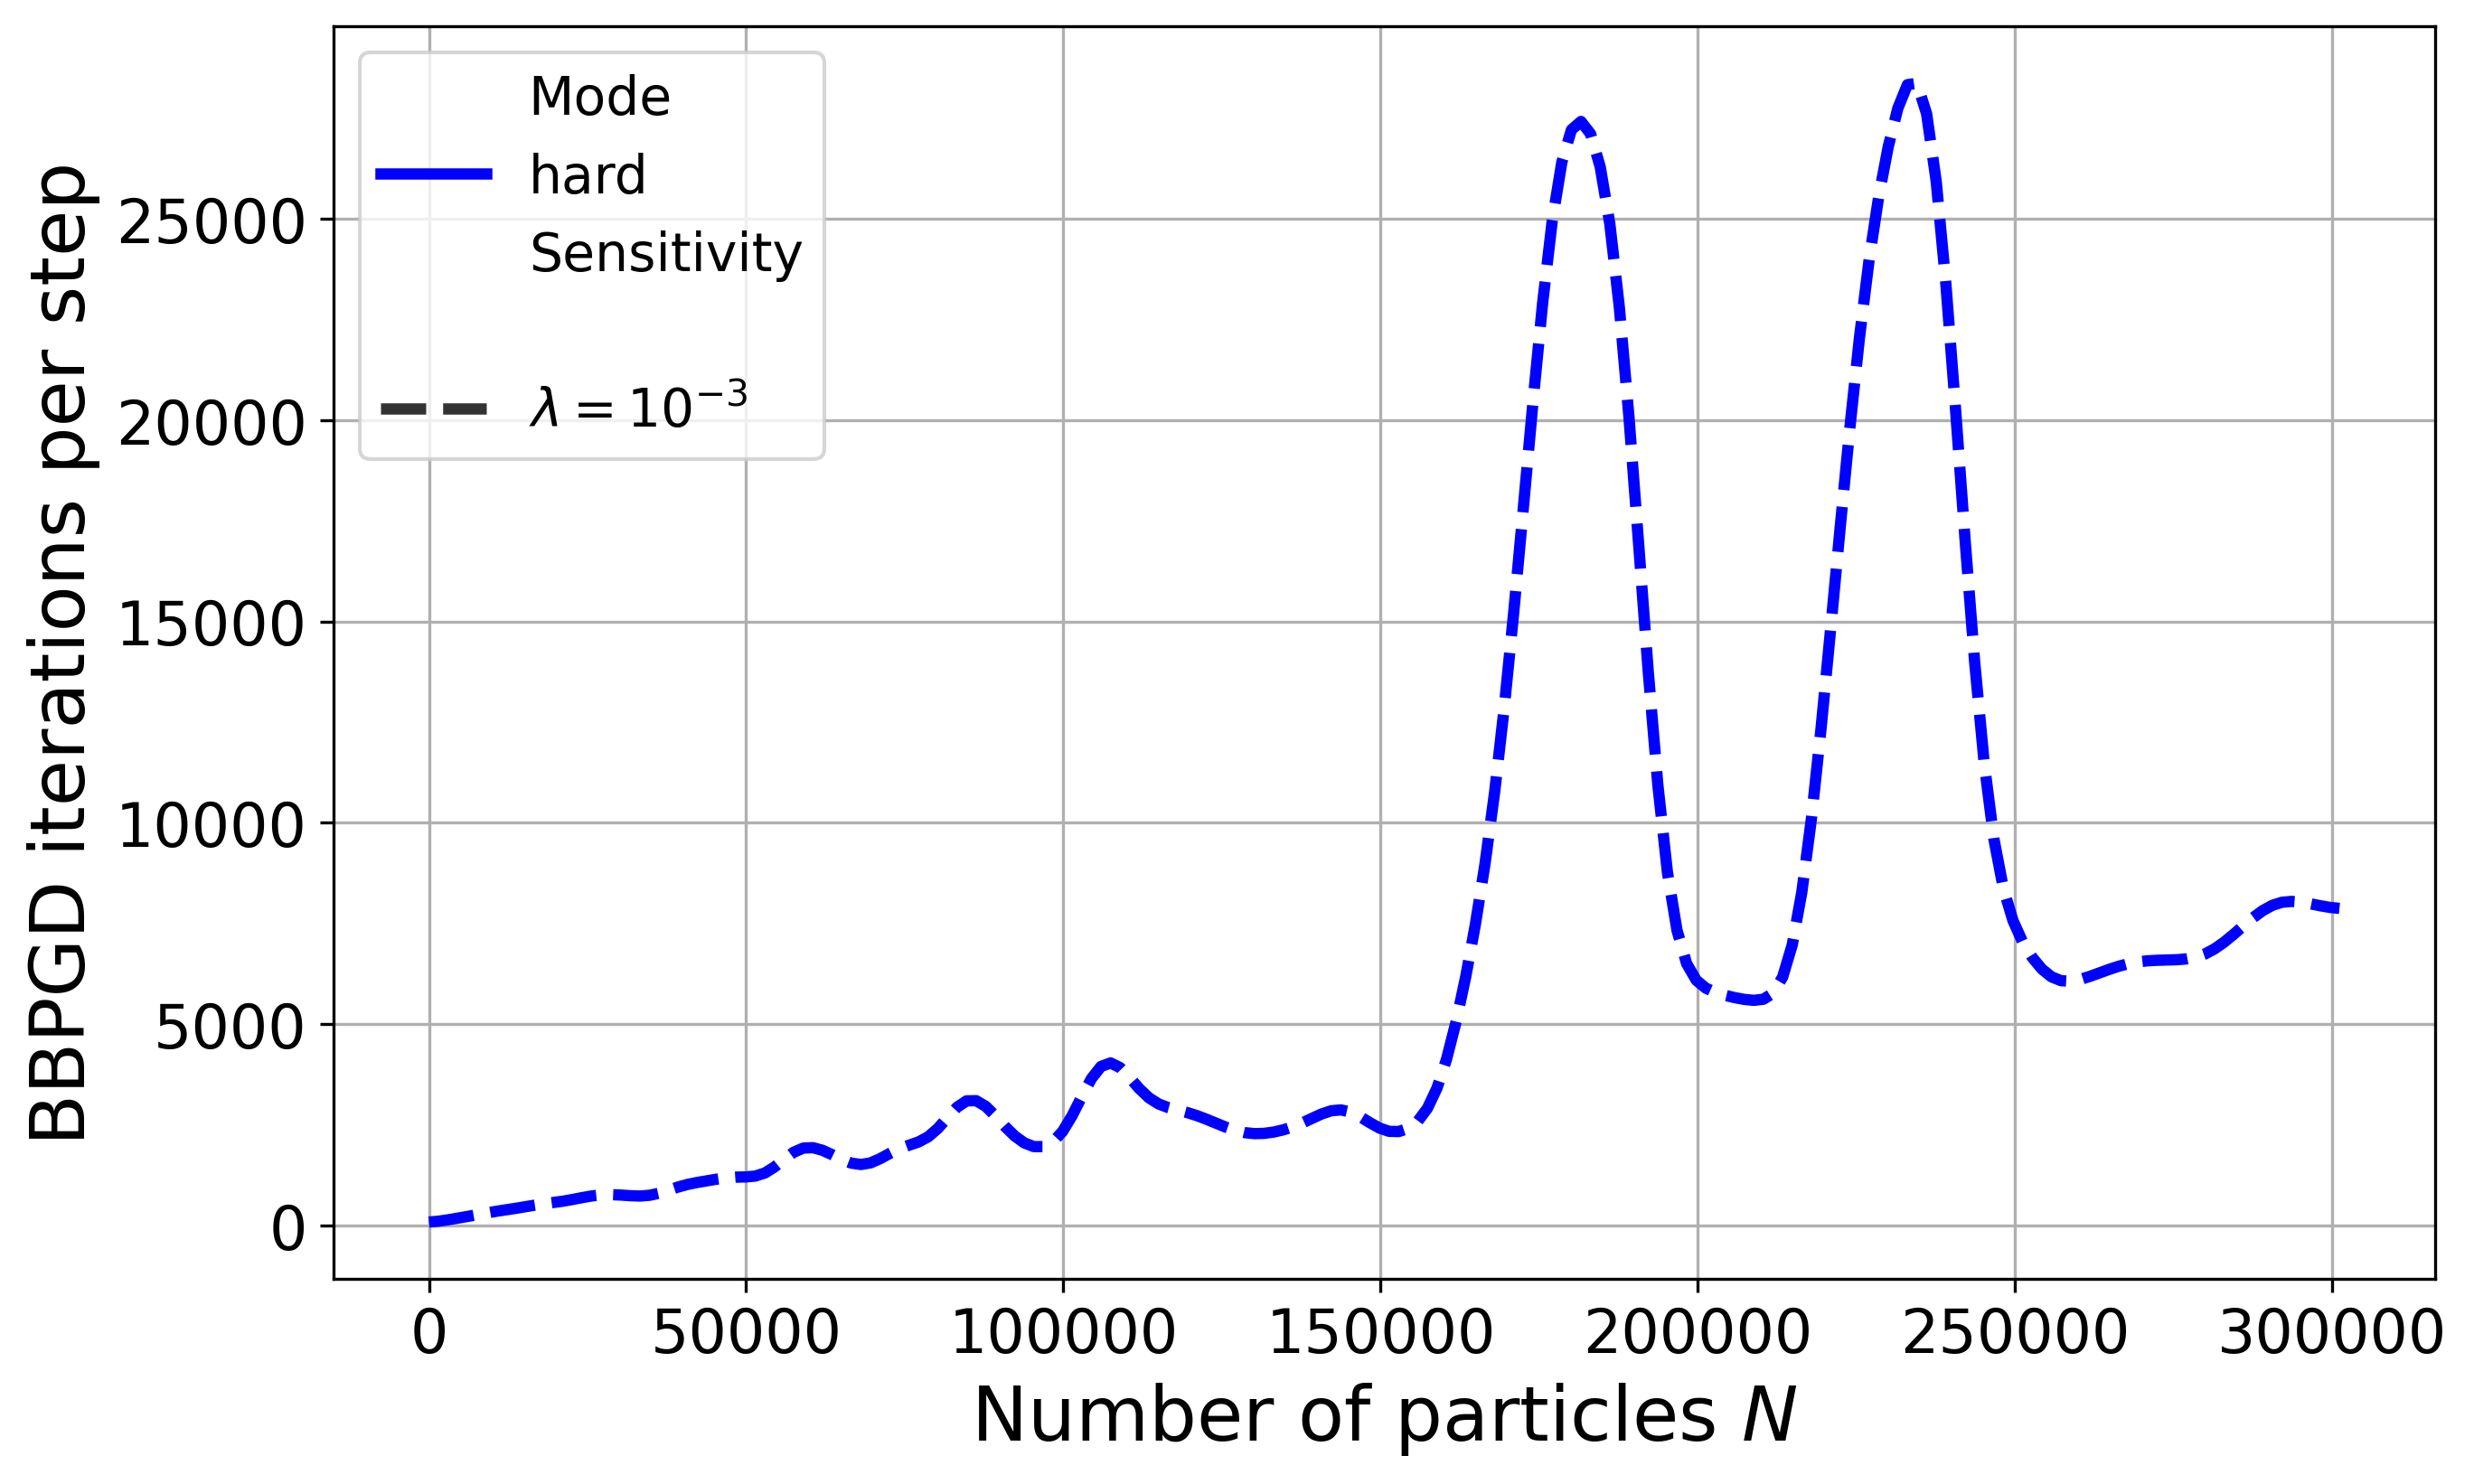
\includegraphics[width=0.8\textwidth]{figures/figures_paper/huge/huge_bbpgd_iterations_per_step_vs_num_particles.png}
    \end{figure}

    \begin{itemize}
        \item Dominates runtime (90\% of computation)
        \item Scales roughly linearly with particle count
    \end{itemize}

\end{frame}


\begin{frame}
    \frametitle{Maximum Colony Visualization ($R = 260$, 301k cells)}

    % Suggest: Show video of largest simulation here
    % \movie[width=0.9\textwidth]{}{huge_colony_growth.mp4}

    \vspace{-0.3cm}
    \begin{figure}
        \centering
        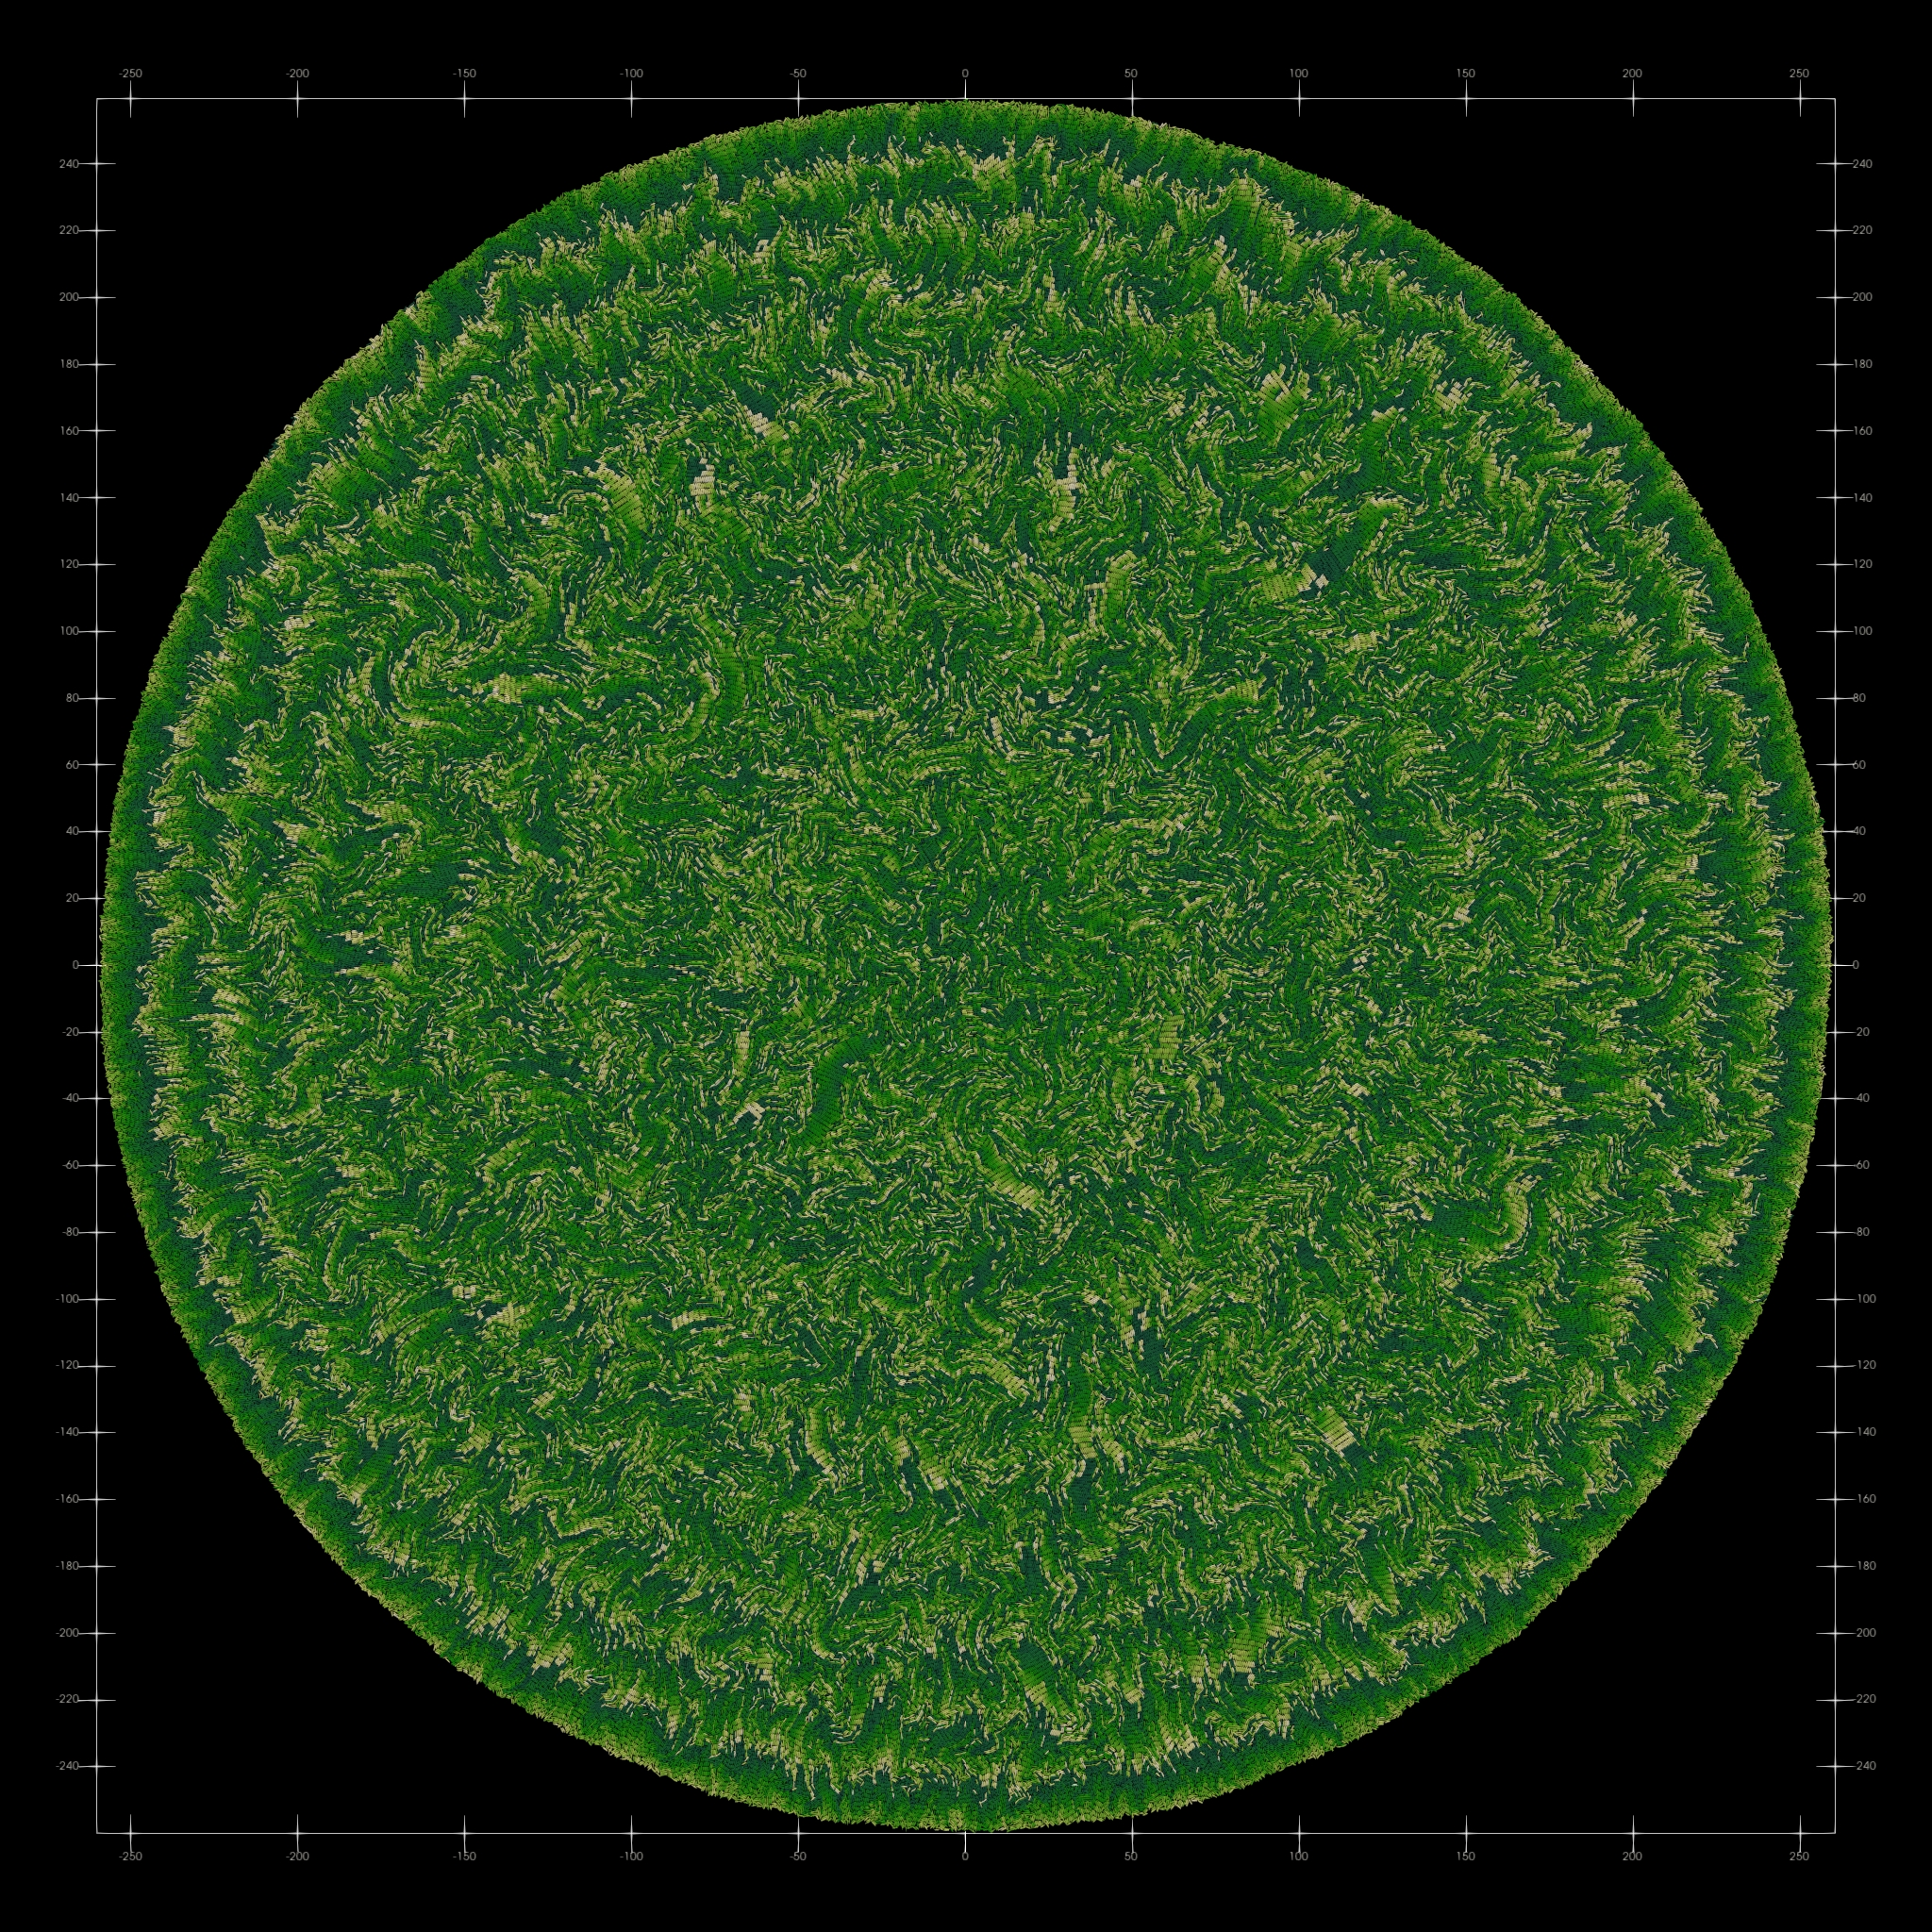
\includegraphics[width=0.6\textwidth]{figures/figures_paper/huge/huge_hard.jpeg}
    \end{figure}

\end{frame}


% ============================================================
% SECTION 7: SYNTHESIS & CONCLUSIONS
% ============================================================

\section{Discussion}

\begin{frame}
    \frametitle{Model Comparison Summary}

    \vspace{-0.5cm}
    \begin{table}
        \centering
        \begin{tabular}{lcccc}
                                              & \multicolumn{2}{c}{\textbf{Soft}} & \multicolumn{2}{c}{\textbf{Hard}}                                              \\
            \cmidrule(lr){2-3} \cmidrule(lr){4-5}
            \textbf{Criterion}
                                              & \shortstack{Small                                                                                                  \\Colonies}
                                              & \shortstack{Large                                                                                                  \\Colonies}
                                              & \shortstack{Small                                                                                                  \\Colonies}
                                              & \shortstack{Large                                                                                                  \\Colonies} \\
            \midrule
            \multicolumn{5}{l}{\textit{Biological Fidelity:}}                                                                                                      \\
            $\quad$  Ring formation           & \cmark                            & \cmark                            & \cmark        & \cmark                     \\
            $\quad$  Packing density          & \cmark                            & \xmark                            & \cmark        & \cmark                     \\
            $\quad$  Microdomain quality      & \cmark                            & \xmark                            & \cmark        & \cmark                     \\
            \midrule
            \multicolumn{5}{l}{\textit{Performance:}}                                                                                                              \\
            $\quad$ Runtime                   & \cmark \cmark                     & \xmark \xmark \textup{*}          & \cmark        & \cmark \cmark              \\
            $\quad$ Parallel scalability      & \xmark                            & \cmark \cmark \textup{*}          & \xmark        & \cmark \cmark              \\
            $\quad$ Implementation complexity & \cmark \cmark                     & \cmark \cmark                     & \emoji{skull} & \emoji{skull}\emoji{skull} \\
        \end{tabular}
    \end{table}

    \vspace{0.3cm}
    \footnotesize{\textup{*} Actual soft model performance degrades significantly due to timestep reduction.}

\end{frame}

\begin{frame}
    \frametitle{When to use each Model?}

    \vspace{-0.1cm}
    \begin{block}{Hard Model (Recommended for most applications)}
        \textbf{Use when:}
        \begin{itemize}
            \item Accurate stress distributions needed
            \item Cell-scale phenomena matter
            \item Realistic packing required
        \end{itemize}

        \textbf{Advantages:} Superior performance, physical accuracy
    \end{block}

    \begin{block}{Soft Model (Limited use cases)}
        \textbf{Only consider when:}
        \begin{itemize}
            \item Preliminary exploration of small systems ($R \lesssim 50$)
            \item Only macroscopic patterns of interest
        \end{itemize}

        \textbf{Warning:} Artifacts limit applicability
    \end{block}

\end{frame}


% ============================================================
% SECTION 8: FUTURE WORK
% ============================================================

\section{Future Directions}

\begin{frame}
    \frametitle{Future Work}

    \begin{enumerate}
        \item \textbf{Hard Model Solver Improvements}
              \begin{itemize}
                  \item Leverage PETSc GPU support
                  \item Warm-start BBPGD with previous solution
              \end{itemize}

              \vspace{0.3cm}

        \item \textbf{Soft Model Enhancements}
              \begin{itemize}
                  \item Consider overlap, in adaptive timestepping.
                  \item Consider alternatives to prevent overlap
                  \item Reduce communication overhead
              \end{itemize}

              \vspace{0.3cm}

        \item \textbf{More Applications}
              \begin{itemize}
                  \item Other cell shapes (soft bodies?)
                  \item More complex models (Nutrient fields?, Outside forces?)
                  \item Utilize 3D capabilities
              \end{itemize}
    \end{enumerate}

\end{frame}


% ============================================================
% CONCLUSIONS
% ============================================================

\section*{Conclusions}

\begin{frame}
    \begin{center}
        \vspace{1cm}
        {\LARGE \textbf{Thank you for your attention!}}

        \vspace{1.5cm}

        \Huge{Questions?}

        \vspace{1.5cm}

        \normalsize
        \texttt{manuel.lerchner@tum.de}

        \vspace{0.3cm}

        \small
        Code: \url{https://github.com/manuellerchner/MicrobeGrowthSim-IDP}

        \vspace{0.2cm}

        Supplementary materials: \url{https://home.cit.tum.de/~ler/bacteria/}
    \end{center}
\end{frame}

\begin{frame}[allowframebreaks, noframenumbering]
    \frametitle{References}
    \footnotesize
    \bibliographystyle{apalike}
    \bibliography{../latex/literature}
\end{frame}

% ============================================================
% BACKUP SLIDES
% ============================================================

\appendix

\begin{frame}
    \frametitle{Backup: BBPGD Convergence}

    \begin{figure}
        \centering
        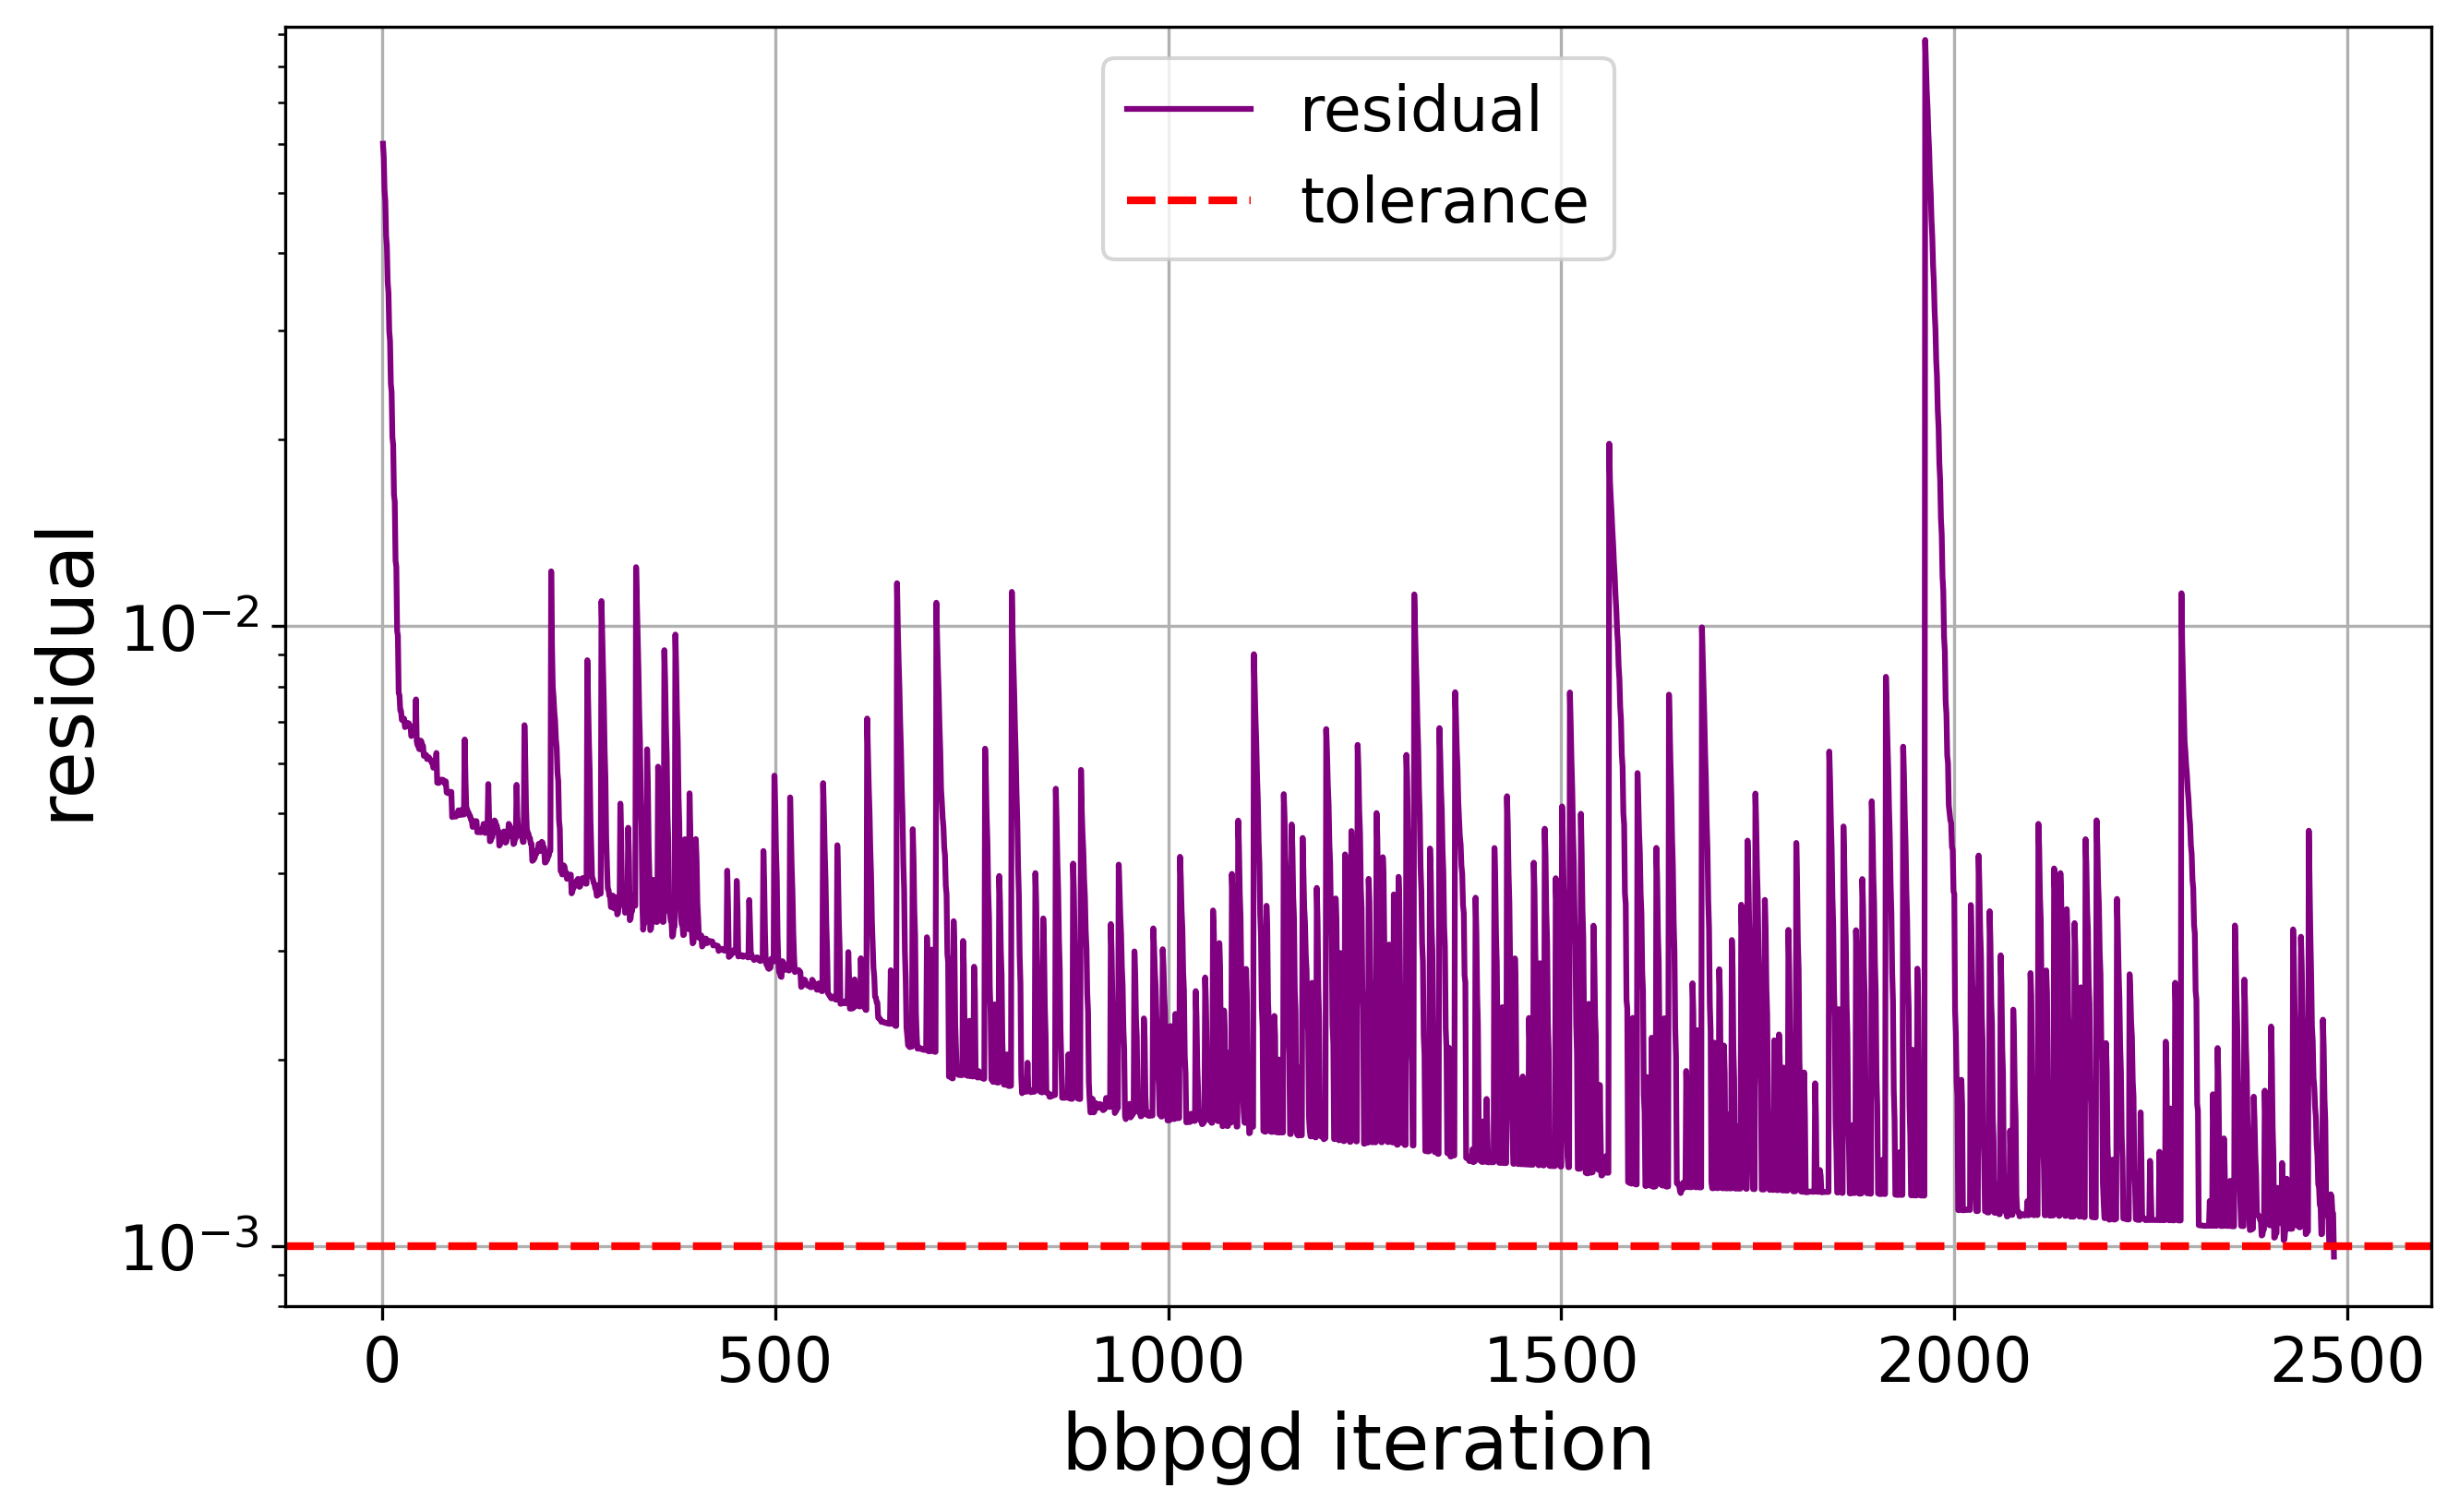
\includegraphics[width=0.9\textwidth]{figures/figures_paper/bbpgd/bbpgd_residual.png}
    \end{figure}

\end{frame}

\begin{frame}
    \frametitle{Backup: BBPGD Energy Evolution}

    \begin{figure}
        \centering
        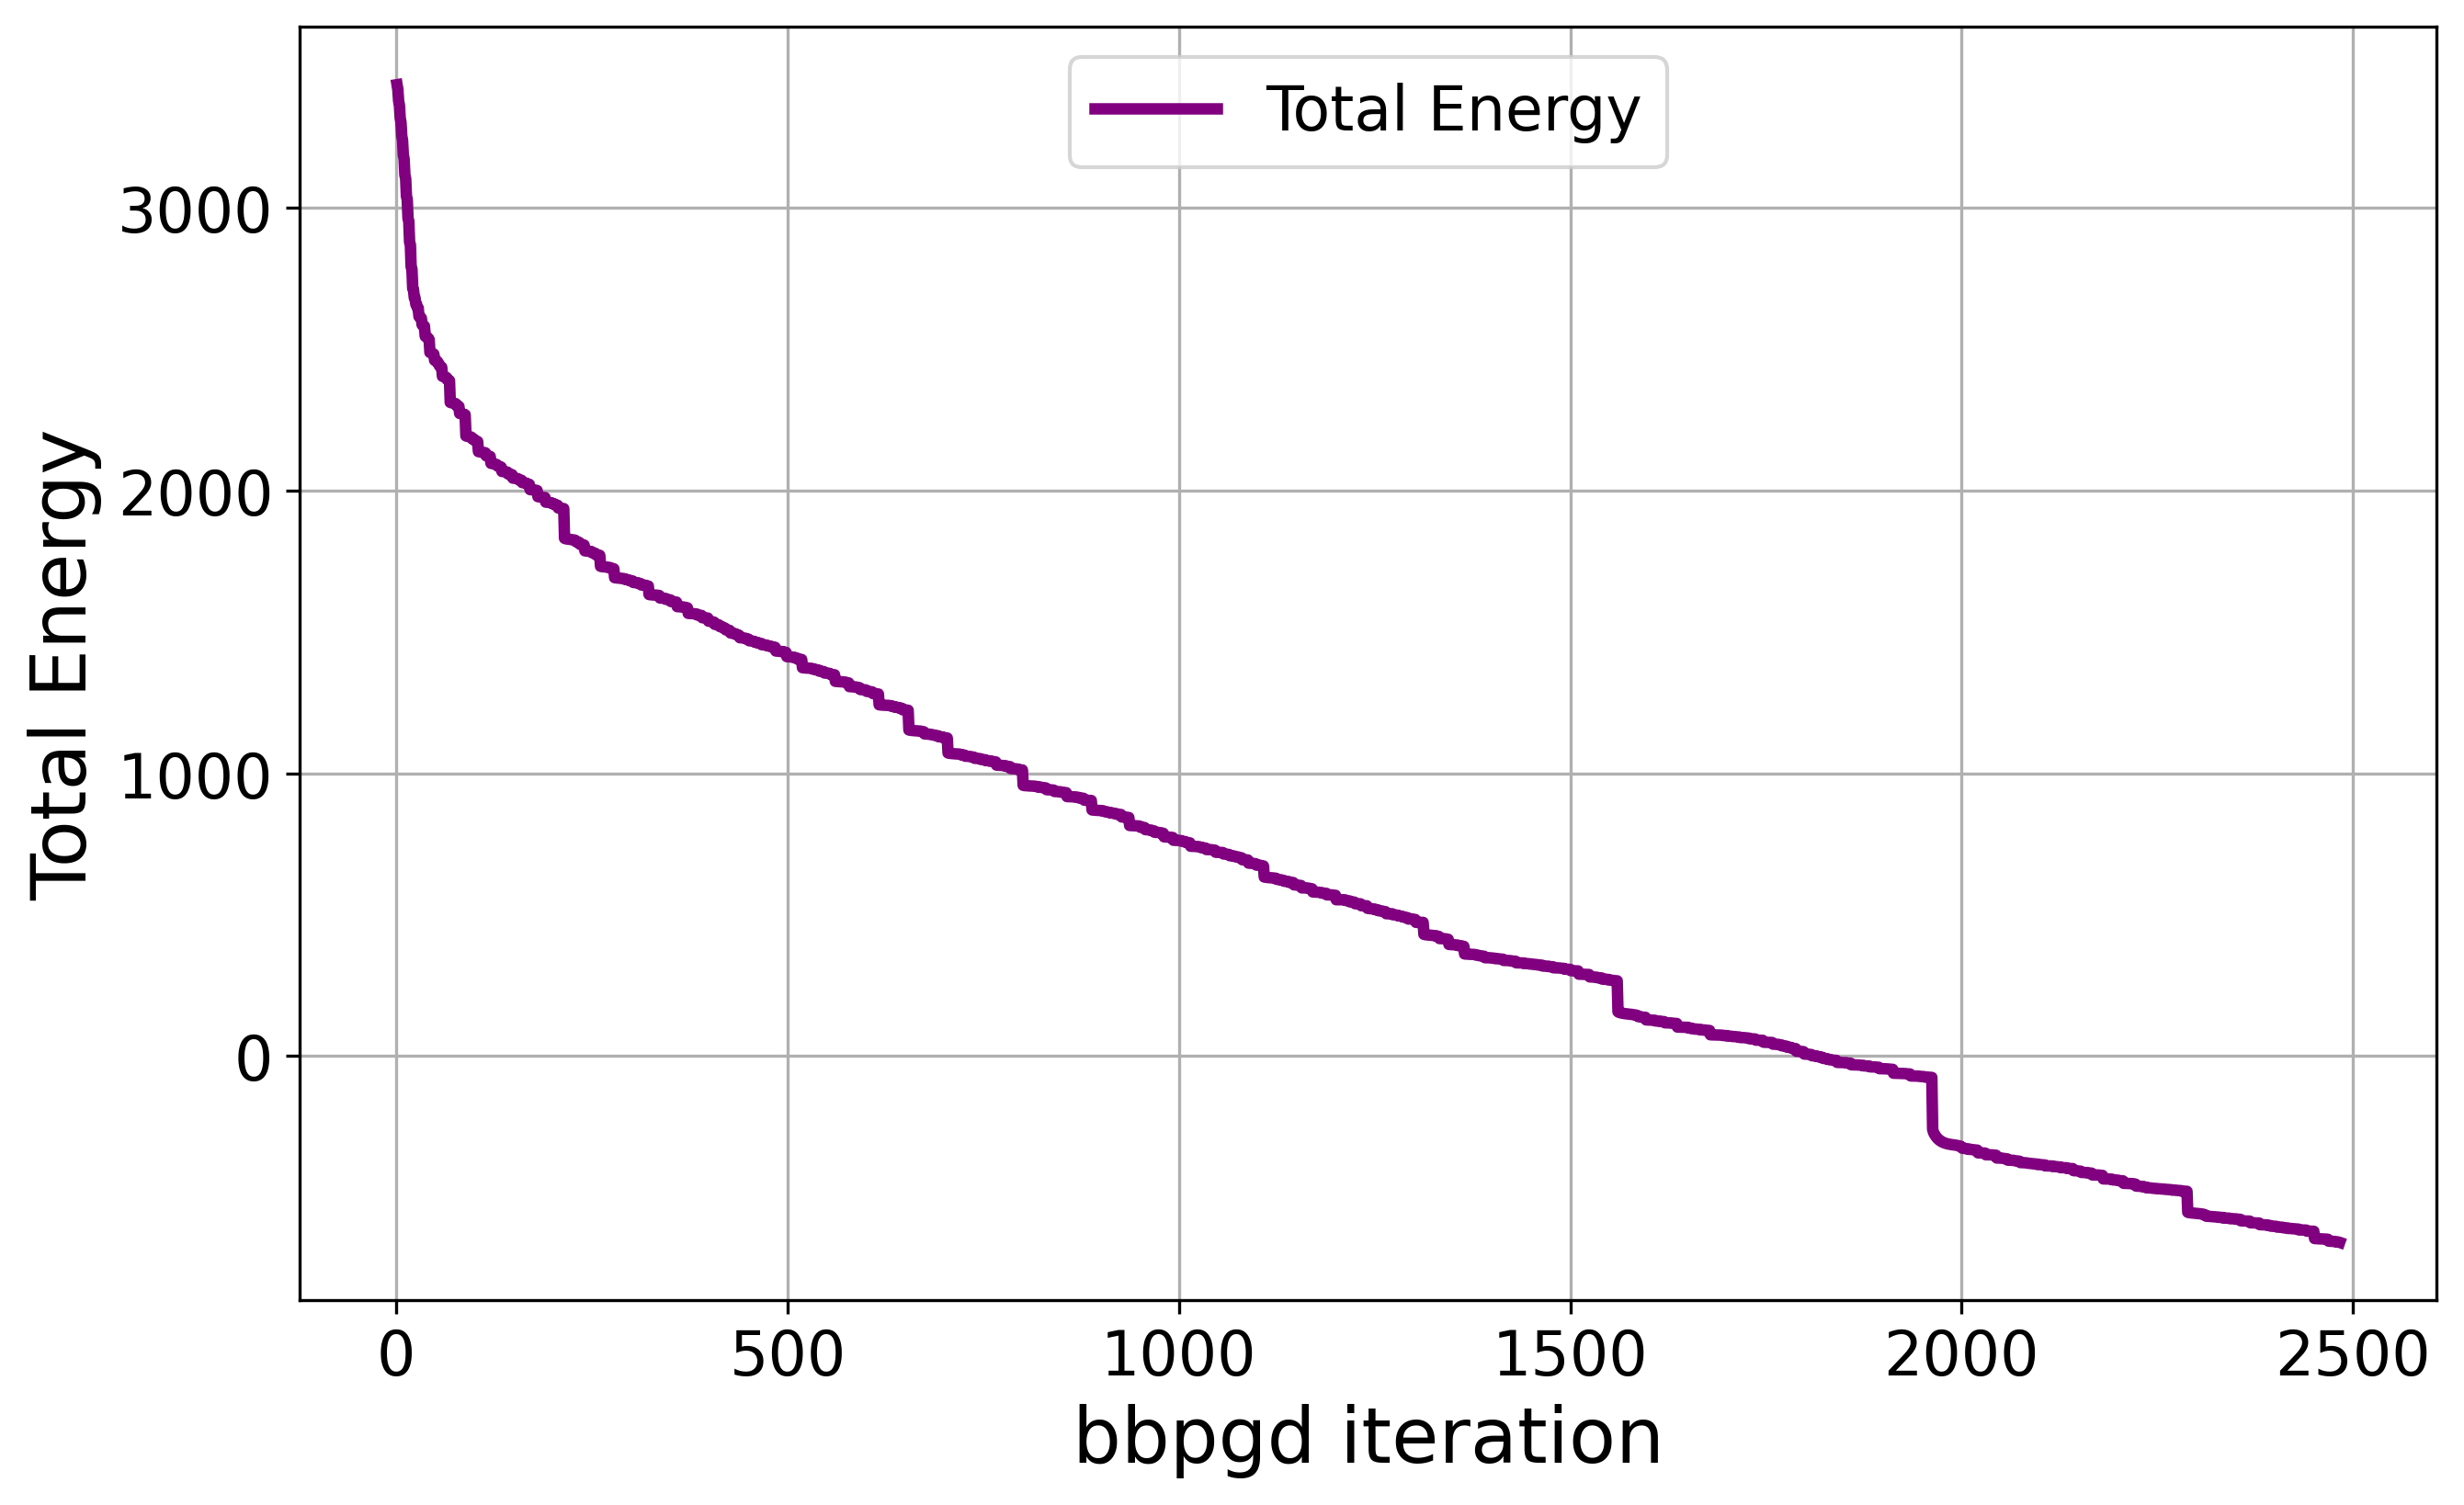
\includegraphics[width=\textwidth]{figures/figures_paper/bbpgd/bbpgd_total_energy.png}
    \end{figure}

\end{frame}

\end{document}